\newpage
\chapter{Measurement of Higgs boson self-coupling}
\label{HHyybb}

The central subject of this thesis is to search for di-Higgs boson events decaying into \HHyybb using the full Run-2 data sample. The absence of a significant number of signal events is translated into a measurement of the Higgs boson self-coupling. All the ingredients needed to select and reconstruct the \HHyybb events were presented in the previous chapters. This chapter describes the analysis strategy to measure the Higgs boson self-coupling, the results and their comparison to the previous ATLAS publication with 36 \ifb of data and the CMS full Run-2 results.  
%This chapter should include the HH analysis and \kl limits

\section{Data and simulation}
\label{HHyybb:Data&MC}
As mentioned before, the analysis uses the full Run-2 dataset recorded by the ATLAS experiment between 2015 and 2018 corresponding to a total integrated luminosity of 139 $\pm$ 2.4 \ifb (Figure \ref{fig:chap2:LHC:Lumi}). The values of the integrated luminosity recorded in each year are shown in Table \ref{tab:HHyybb:Data&MC:Lumi} \cite{Lumi}. \\
\begin{table}[htbp]
    \centering
    \begin{tabular}{lc}
    \hline\hline
        Year & int. luminosity [\ifb]  \\ \hline
        2015-2016 & 36.21 \\
        2017      & 44.39 \\
        2018      & 58.45 \\
        \hline \hline
    \end{tabular}
    \caption{Integrated luminosity recorded by ATLAS in Run 2 per year of data taking.}
    \label{tab:HHyybb:Data&MC:Lumi}
\end{table}
\\
Similarly to the $H\rightarrow\gamma\gamma$ analysis, the \HHyybb analysis relies on different sets of di-photon triggers for each year. The trigger used for 2015-2016 requires at least two photons with \eT greater than 35 GeV for the leading and 25 for the sub-leading photon, both passing the loose identification criterion. The di-photon trigger used in 2017-2018 requires at least two photons with the same requirement on their transverse energies but passing the medium identification criterion to reduce fake rates. Figure \ref{fig:HHyybb:Data&MC:Trig} shows the di-photon trigger efficiency for each year as a function of photon \eT and $\eta$. Slightly lower efficiencies are observed in 2017–2018 due to the tightening in photon identification. In addition, no significant dependence on $\eta$ is observed in the trigger efficiency, which remains close to 100\%.
\begin{figure}[htbp]
    \centering
    \subfloat[][]{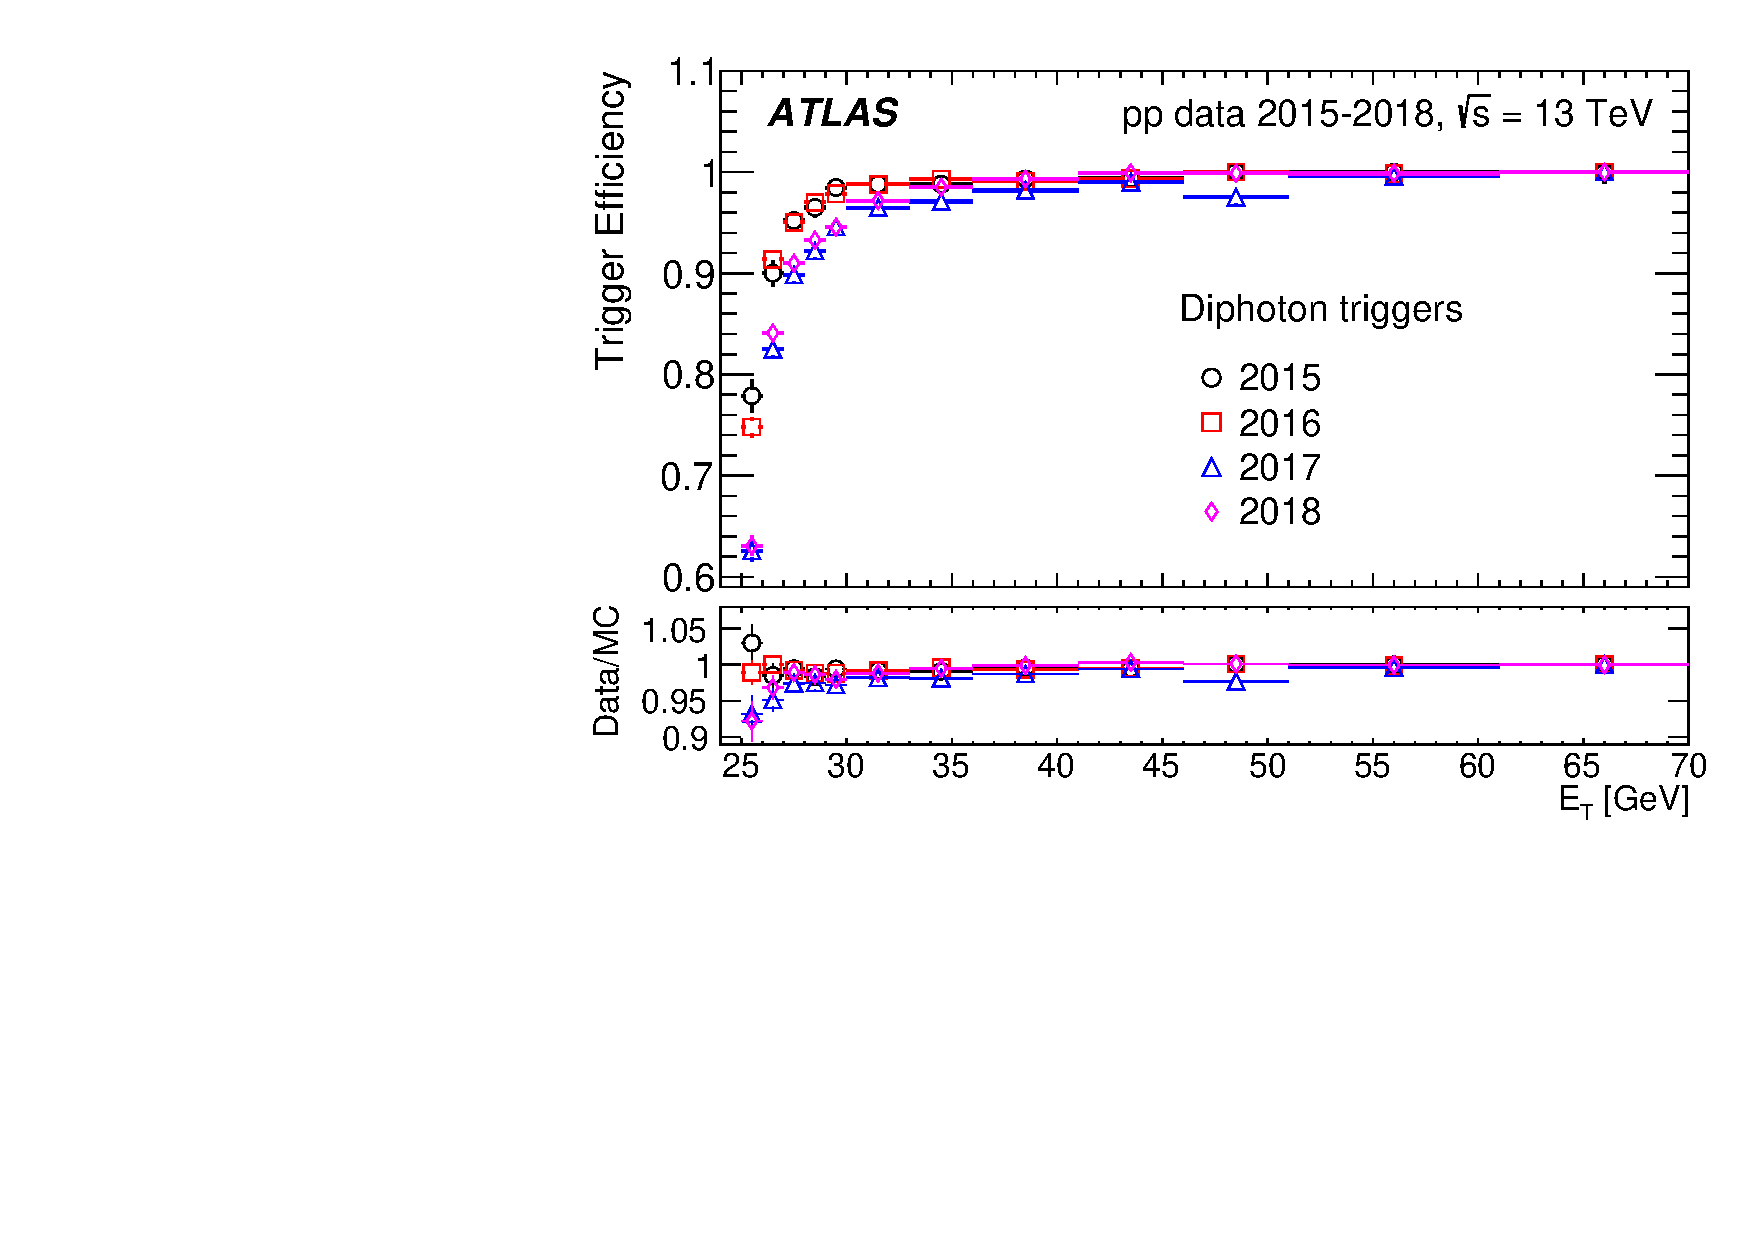
\includegraphics[width=.45\textwidth]{Ch5/Img/Trigger_Et.pdf} }
	\subfloat[][]{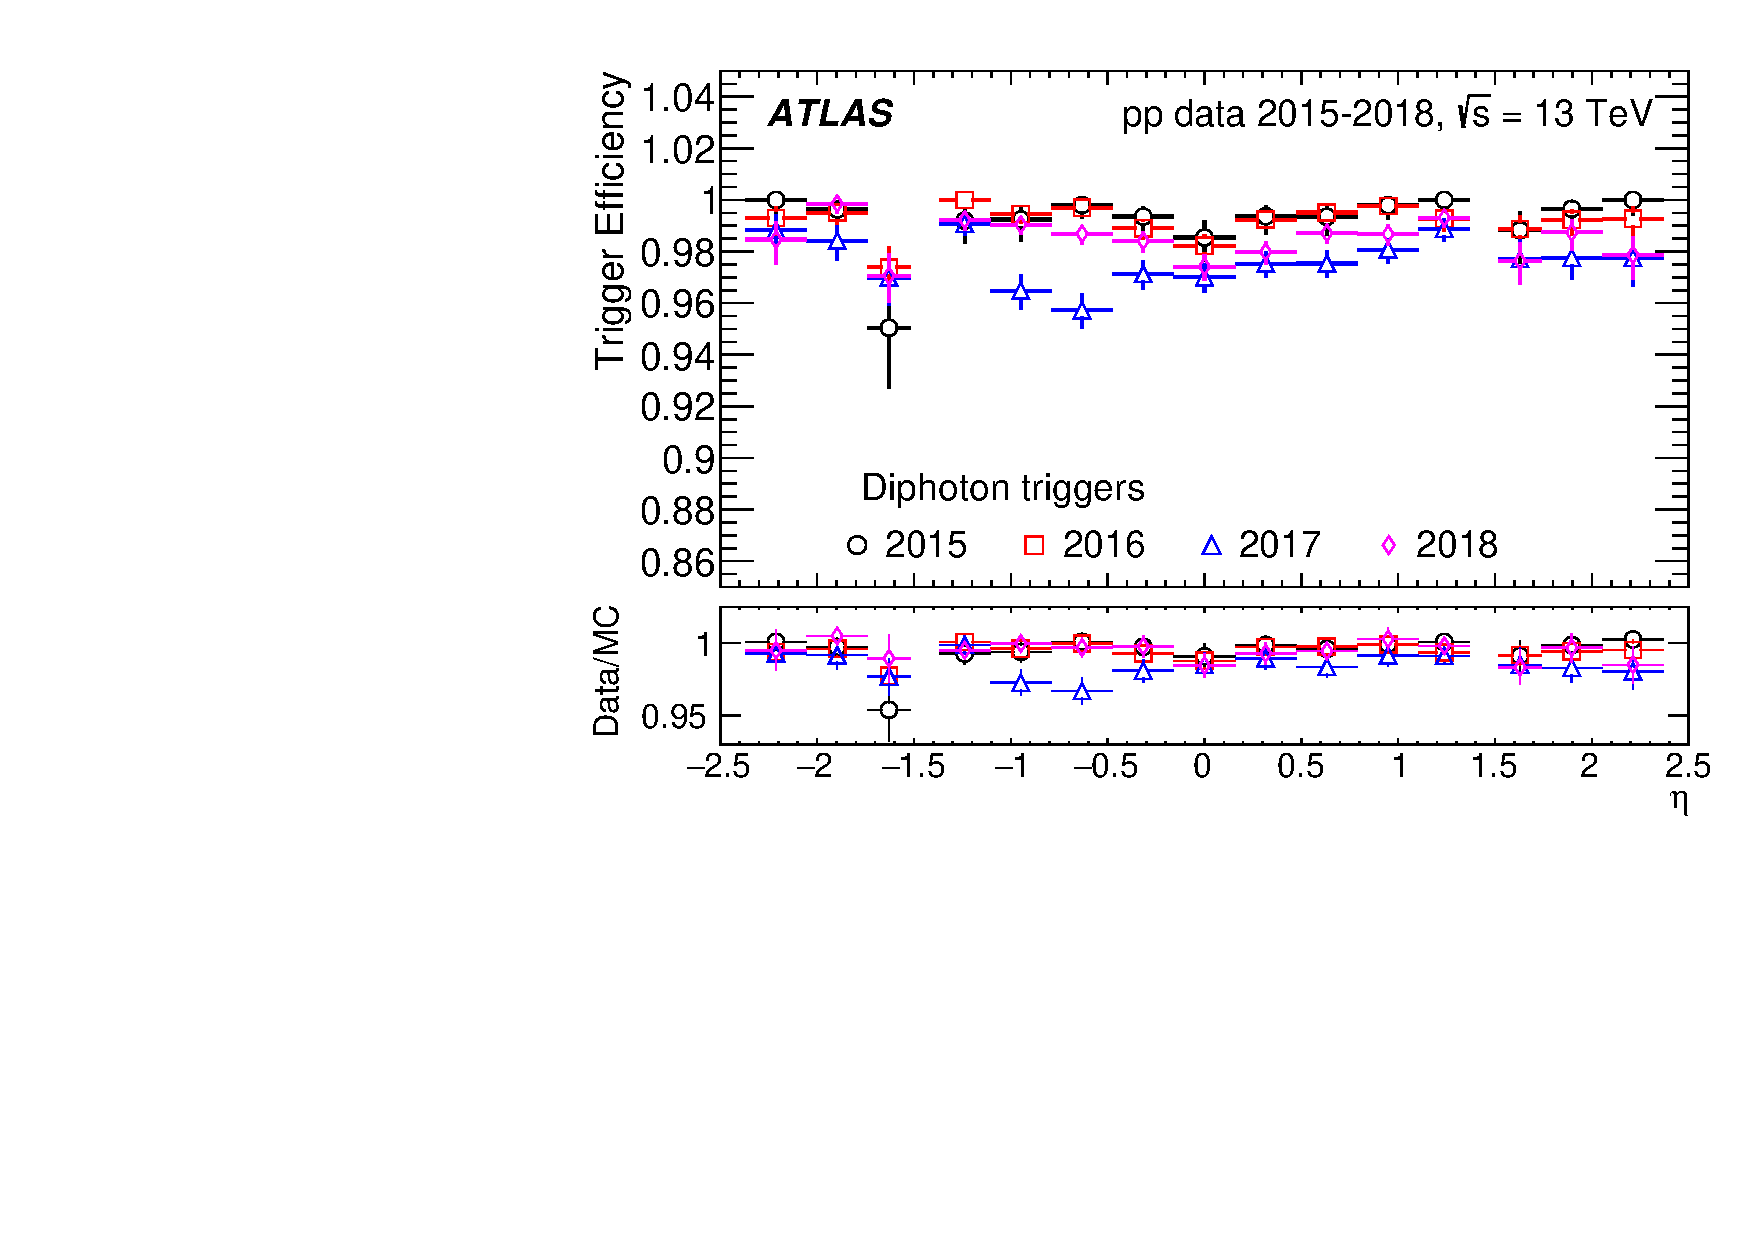
\includegraphics[width=.45\textwidth]{Ch5/Img/Trigger_Eta.pdf}} 
    \caption{Di-photon trigger efficiency in data 2015-2018 as a function of (a) \eT and (b) $\eta$. The ratios of data to MC simulation efficiencies are also shown.}
    \label{fig:HHyybb:Data&MC:Trig}
\end{figure}
\\
For boosted Higgs bosons ($p_T^{Higgs} > $ 650 GeV), two high momentum single-photon triggers available in 2018 were added in a logical OR with the di-photon trigger, requiring a loose photon with an energy of 120 GeV and 140 GeV respectively. The high momentum single-photon triggers have no impact on the HH analysis, since only 0.1\% of signal events pass this trigger. The efficiency of the trigger selection is $\sim$ 83\% for the HH signal, and the selection criteria remains looser than the final analysis selection. 
\\

The simulated \HHyybb sample (MC) are generated for two production modes: the ggF HH and VBF HH productions described in Section \ref{chap1:HH:HPD}. Events from ggF HH production were generated at NLO using the \textsc{Powheg-Box} v2 generator in the finite top-quark mass approximation with PDFLHC15 PDF set \cite{HH_FT, HH_Powheg, PDF4LHC}. The \textsc{PYTHIA} 8.2 code is used for parton showering. Two samples were generated for \kl= 1 and \kl= 10. Events from the VBF HH production were generated at LO  using \textsc{MadGraph5\_aMC@NLO} \cite{HH_VBF} with the \texttt{NNPDF3.0nnlo} PDF set \cite{VBF_PDF} and \textsc{PYTHIA} 8.2 for showering. \\

A reweighting procedure was developed for both ggF and VBF to avoid generating simulation samples for each \kl. Truth level HH samples with 10 million events were produced for \kl= 0, 1, 10 and 20 with specific HH decay modes. A linear combination of samples with \kl= 0, 1 and 20 derived from Eq. \ref{eq:chap1:HH:XSEC:Param} is implemented to derive the sample at a given \kl value. The method was validated for \kl= 10. The total cross-section as a function of \kl and \kt is parameterized as:
\begin{equation}
    \left|A\left(\kappa_{t}, \kappa_{\lambda}\right)\right|^{2}=\kappa_{t}^{2}\left[\left(\kappa_{t}^{2}+\frac{\kappa_{\lambda}^{2}}{20}-\frac{399}{380} \kappa_{t} \kappa_{\lambda}\right)|A(1,0)|^{2}+\left(\frac{40}{38} \kappa_{t} \kappa_{\lambda}-\frac{2}{38} \kappa_{\lambda}^{2}\right)|A(1,1)|^{2}+\frac{\kappa_{\lambda}^{2}-\kappa_{t} \kappa_{\lambda}}{380}|A(1,20)|^{2}\right],
\end{equation}
with weights derived by dividing the binned $m_{HH}$ distribution of the target \kl by the binned $m_{HH}$ distribution of the SM sample. A bin width of 10 GeV is adopted and \kt= 1. For each \kl value, the inclusive cross-section is normalized to its theoretical prediction \cite{LHE}. The reweighting procedure is common across all HH analyses and has been validated for \HHyybb by comparing the $m_{\gamma\gamma}$ and event yields in the generated \kl= 10 and the reweighted \kl= 1 to \kl= 10. A good agreement is found with a maximum discrepancy of 3-4\% taken as systematic uncertainty related to the method.  \\ 

For background processes, different generators were used depending on the process. Only the $H\to\gamma\gamma$ decay channel is considered for single Higgs boson backgrounds. An alternative showering with \textsc{Herwig}7 for the single Higgs boson backgrounds is used to estimate the systematic uncertainties of the parton shower. Table \ref{tab:HHyybb:Data&MC:Samples} lists the generators, parton showering and PDF used for each component. 
\begin{table}[htbp]
  \centering
    \begin{tabular}{ cccc }
    \hline\hline
    Process & Generator & PDF set  & Showering    \\
       \hline
        ggF  & NNLOPS & PDFLHC &  \textsc{PYTHIA} 8.2  \\
        VBF & \textsc{Powheg-Box} v2 & PDFLHC  &  \textsc{PYTHIA} 8.2        \\
        $WH$ & \textsc{Powheg-Box} v2 & PDFLHC  &  \textsc{PYTHIA} 8.2 \\
        $q\bar{q}\to ZH$ & \textsc{Powheg-Box} v2 &  PDFLHC  &  \textsc{PYTHIA} 8.2 \\
        $gg\to ZH$ &  \textsc{Powheg-Box} v2 & PDFLHC  &  \textsc{PYTHIA} 8.2  \\
        $t\bar{t}H$ & \textsc{Powheg-Box} v2 & \texttt{NNPDF2.3lo} & \textsc{PYTHIA} 8.2  \\
        $bbH$ &  \textsc{Powheg-Box} v2 & \texttt{NNPDF3.0nnlo}  &  \textsc{PYTHIA} 8.2     \\
        $tHqj$ & \textsc{MadGraph5\_aMC@NLO} &  \texttt{NNPDF3.0nnlo}  & \textsc{PYTHIA} 8.2   \\
        $tHW$  & \textsc{MadGraph5\_aMC@NLO} &  \texttt{NNPDF3.0nnlo}  & \textsc{PYTHIA} 8.2   \\
         $\gamma\gamma+$jets &   \texttt{SHERPA}~v2.2.4 & \texttt{NNPDF3.0nnlo}  &  \texttt{SHERPA}~v2.2.4  \\
         $t\bar{t} \gamma \gamma$ & \textsc{MadGraph5\_aMC@NLO}  &  \texttt{NNPDF2.3lo} & \textsc{PYTHIA} 8.2 \\
        \hline\hline
    \end{tabular}
    \caption{Summary of single Higgs boson background samples, split by production modes, and continuum background samples. The generators used, and the PDF sets are also listed. }
  \label{tab:HHyybb:Data&MC:Samples}
\end{table}
\\
The dominant background is the reducible continuum $\gamma\gamma+$jets process which is not evaluated from the generated \texttt{SHERPA} sample. Instead a data-driven method is implemented to estimate its contribution by parametrizing its shape with an analytical function fit, which its form is fixed using the simulated \texttt{SHERPA} sample.

\section{Object and event selection}
\label{HHyybb:ObjEvt}

\subsection{Object selection}
\label{HHyybb:ObjEvt:Obj}

\subsubsection{Di-photons}
\label{HHyybb:ObjEvt:Obj:gamma}
The selected photons are reconstructed using the dynamical topological clusters method, as defined in Section \ref{chap2:Objects:Egamma}, and must fulfil a pre-selection of $p_T > $ 25 GeV and $|\eta| < $ 2.37 (excluding the transition region). They are calibrated using the latest Run-2 calibration correction for the energy scale and resolution as detailed in Section \ref{chap2:Objects:Egamma:Cal}. Photons are required to pass the tight identification as defined in Section \ref{gamma:ID}. Events must contain at least two photons ($N_{\text{photons}} \geq $ 2). The $H\to\gamma\gamma$ candidate is reconstructed from the two highest $p_T$ photons in the event.\\ 
The two photons are used to re-determine the primary vertex using an algorithm based on NNs that makes use of the pointing information from the electromagnetic calorimeter along with tracking information \cite{DiPhotonVertex}. Track-based isolation quantities are re-computed based on the defined primary vertex. \\
A loose isolation criterion is applied to select isolated photons as described in Section \ref{gamma:Iso}.\\
The selected Higgs bosons candidates must pass an additional selection which reflects the online trigger. It requires that the leading (subleading) photon $p_T$ is at least 35\% (25\%) of the invariant mass of the two photons. A mass window cut in the range [105, 160] GeV is also applied, thus the cut on the leading (subleading) photon momentum fraction translates in a cut on its energy to be larger than at least 36.75 (26.25) GeV.

\subsubsection{Leptons as veto}
\label{HHyybb:ObjEvt:Obj:lepton}

Electron candidates are required to have $p_T > $ 10 GeV and $|\eta| < $ 2.47 (excluding the transition region). Additionally, they should pass the medium identification and tight isolation as defined in Sections \ref{chap2:Objects:Egamma:EID} and \ref{chap2:Objects:Egamma:EIso}. \\
Muon candidates are required to have $p_T > $ 10 GeV, $|\eta| < $ 2.7 and required to satisfy a medium identification and loose isolation. Both the electrons and muons are matched to the primary vertex via requirements on the track longitudinal and transverse impact parameters, $|z_0|$ and $|d_0|$.

\subsubsection{Jets}
\label{HHyybb:ObjEvt:Obj:Jet}
As described in Chapter \ref{Jet}, particle flow jets are adopted for this analysis. They are required to have $|\eta| < $ 2.5 and $p_T > $ 25 GeV. A tight JVT is applied to separate jets arising from the hard-scatter and those from pile-up, as defined in Section \ref{Jet:Tag}. The selected jets are calibrated using the calibration chain described in Section \ref{Jet:Cal}. \\
The jet flavour is determined using the 77\% efficiency WP of the DL1r tagger as described is Section \ref{Jet:Tag:Dlr}. Events are required to have exactly two $b$-jets ($N_{\text{b-jet}}^{77\%} = $ 2) to preserve the orthogonality with the HH$\to$\bbbb channel. The two $b$-jets are used to reconstruct the $H\to\bar{b}b$ candidate. \\
The energy of $b$-tagged jets is corrected with the calibration method introduced in Section \ref{Jet:Cal:BCal}. The improvement on the \mbb resolution translates to a 7.2\% $\pm$ 2\% improvement in the expected signal significance (the error is estimated using the bootstrap method \cite{Bootstrap}). \\

An additional 5-10\% improvement on the \mbb resolution could have been achieved through the use of a likelihood-based kinematic fit denoted "kinematic fit". The kinematic fit uses the $H\to\gamma\gamma$ component reconstructed with a percent-level precision to improve the $H\to\bar{b}b$ resolution through the constraint of the good overall balance in the transverse plane. I developed the kinematic fit for this \HHyybb analysis. It is not used in the final analysis as a bug was found in its implementation after sample production. Fixing the bug would have delayed the publication. A detailed description of the kinematic fit can be found in Appendix \ref{Adx4}. \\

%An overlap removal procedure is applied to avoid using same detector signals in the same events. Jets within $\Delta R=$ 0.2 of electron or 0.4 of muon are removed.

\subsection{Event selection}
\label{HHyybb:ObjEvt:Evt}
Events are reconstructed from $H\to\bar{b}b$ and $H\to\gamma\gamma$ defined above. In addition to the requirement on the number of photons ($N_{\text{photons}} \geq $ 2) and the $b$-jet veto ($N_{\text{b-jet}}^{77\%} = $ 2), the following criteria are applied to reduce the $t\bar{t}H$ background contamination: 

\begin{itemize}
    \protect
    \item less than six jets in the central detector region ($|\eta| < $ 2.5) to reject $t\bar{t}H$ with the hadronic decays. 
    \item veto any event with at least one lepton to reject $t\bar{t}H$ with leptonic decays.  
\end{itemize}


Selected events are then divided in two regions using the $m_{b\bar{b}\gamma\gamma}^*$ variable, which is defined as  $m_{b\bar{b}\gamma\gamma}^* = m_{b\bar{b}\gamma\gamma} - m_{\bar{b}b} - m_{\gamma\gamma} + 250$ GeV. The $m_{b\bar{b}\gamma\gamma}^*$ was implemented to improve the $m_{HH}$ resolution for the resonant analysis. A high-mass region, with $m_{b\bar{b}\gamma\gamma}^* > $ 350 GeV, targets the SM signal, while a low-mass region, with $m_{b\bar{b}\gamma\gamma}^* < $ 350 GeV, is used to retain sensitivity for BSM signals and provide better constraints on \kl are defined. The distribution of $m_{b\bar{b}\gamma\gamma}^*$ is shown in Figure \ref{fig:HHyybb:ObjEvt:Evt:myybb}.  
\begin{figure}[htbp]
    \centering
	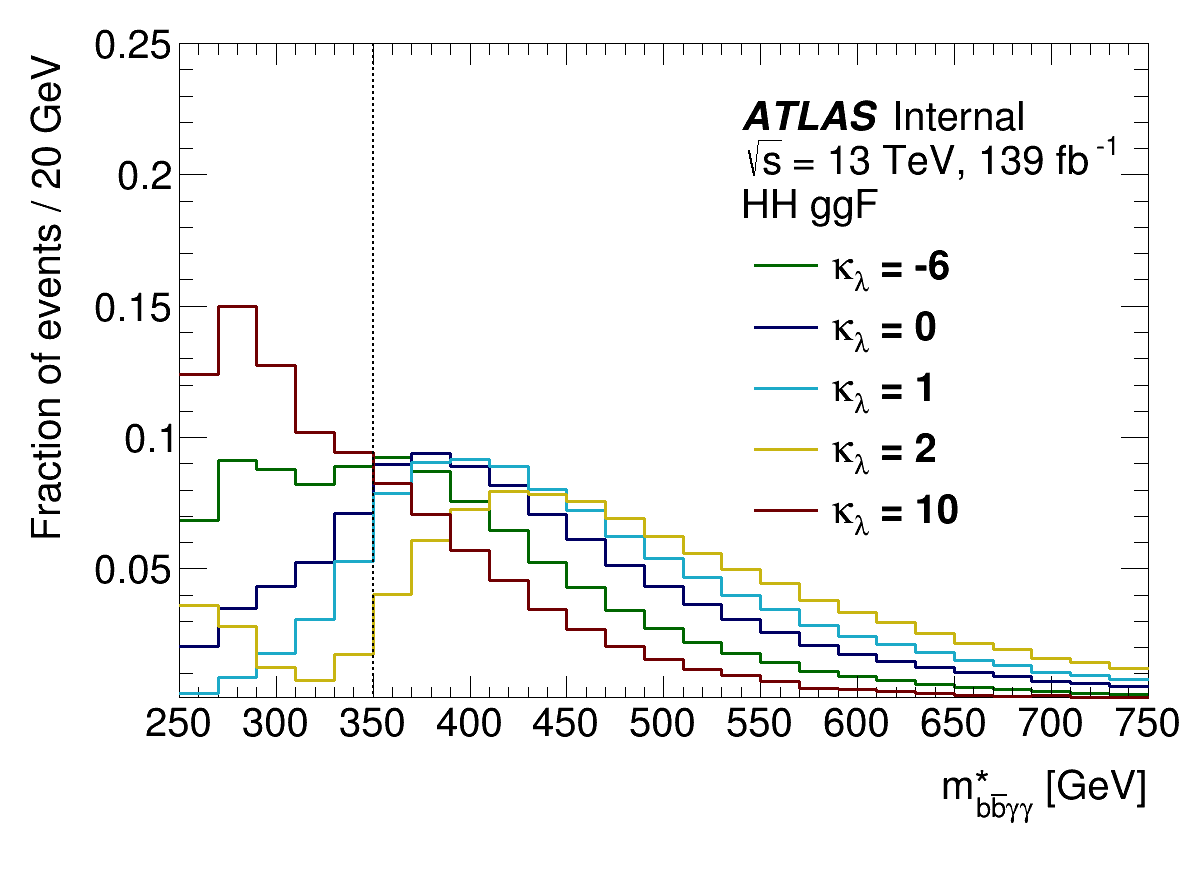
\includegraphics[width=.6\textwidth]{Ch5/Img/yybbstar_ggF.png} 
	%\subfloat[VBF HH production mode][VBF HH production mode]{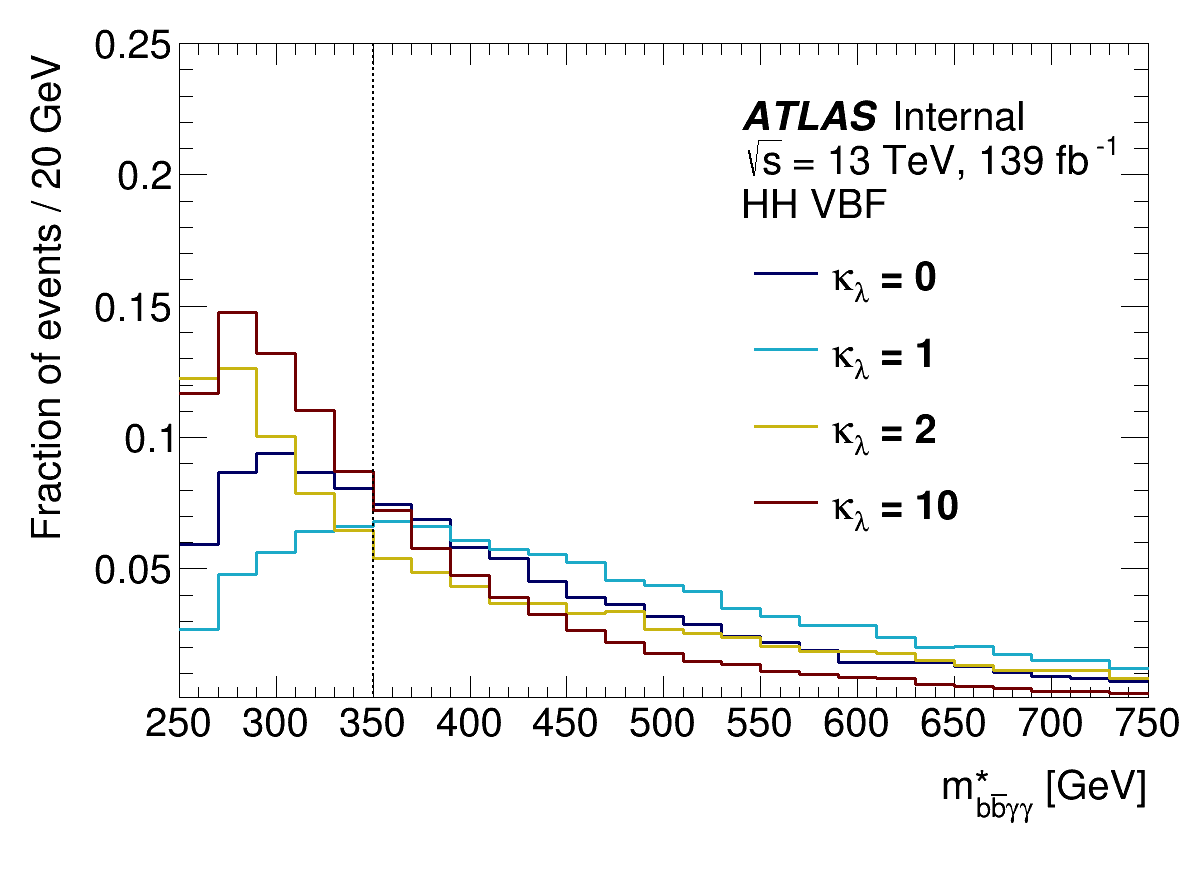
\includegraphics[width=.45\textwidth]{Ch5/Img/yybbstar_VBF.png}} 
    \caption{$m_{b\bar{b}\gamma\gamma}^*$ distributions for the ggF HH signal with several \kl values. $m_{b\bar{b}\gamma\gamma}^* = $ 350 GeV is chosen as the separating boundary between categories targeting the SM and BSM \kl signals.}
    \label{fig:HHyybb:ObjEvt:Evt:myybb}
\end{figure}
\\
In each mass region, a separate BDT is trained using XGBoost \cite{XGBoost} to categorize the ggF HH signal against a combination of the dominant backgrounds (continuum $\gamma\gamma$+jets, $t\bar{t}H$, ggF and ZH). In the high-mass region, the SM \kl= 1 process is considered as the ggF HH signal while in the region targeting BSM scenarios (low-mass) the \kl= 10 process ggF HH is used. Table \ref{tab:HHyybb:ObjEvt:Evt:BDT} lists the BDT input variables which are used for both the low and high-mass regions.
\begin{table}[htbp]
    \centering
    \begin{tabular}{lc}
       \hline \hline
        Variable & Definition \\
        \hline
        $p_T$/\myy &  \pT of the two photon system scaled by its invariant mass \myy. \\
        $\eta$ and $\phi$ & Pseudo-rapidity and azimuthal angle of the two photon system. \\
        \hline 
        $b$-tagging score &  $b$-tagging score of the two jets.\\
        $\eta$, $\phi$ and \pT & \pT, pseudo-rapidity and azimuthal angle of the two jets. \\ 
        $m_{b\bar{b}}$ & $H\to b\bar{b}$ invariant mass. \\
        $H_T$ & Scalar sum of the \pT of the jets in the event. \\
        $\chi_{Wt}$ & Single topness defined in Equation \ref{eq:HHyybb:ObjEvt:Evt:Topness}. \\
        \hline
        $E^{miss}_{T}$ and $\phi$ & Missing transverse momentum and its azimuthal angle. \\
        \hline\hline
    \end{tabular}
    \caption{Input variables used in the BDT.}
    \label{tab:HHyybb:ObjEvt:Evt:BDT}
\end{table}


The "single-topness" variable is defined as: 
\begin{equation}
    \chi_{W t}=\min \sqrt{\left(\frac{m_{j_{1} j_{2}}-m_{W}}{m_{W}}\right)^{2}+\left(\frac{m_{j_{1} j_{2} j_{3}}-m_{t}}{m_{t}}\right)^{2}},
    \label{eq:HHyybb:ObjEvt:Evt:Topness}
\end{equation}

where $m_W = $ 80 GeV, $m_t = $ 173 GeV, and the minimum is taken over all possible combinations of 3 jets in the event. No requirement on the $b$-tagging is applied on the third jet. \\

The BDT discriminant distribution for the low mass and the high mass categories are shown in Figure \ref{fig:HHyybb:ObjEvt:Evt:dBDT}. In each mass region, two categories are defined based on the BDT score resulting in total of four categories as listed in Table \ref{tab:HHyybb:ObjEvt:Evt:Cat}. Defining additional categories does not bring any significant improvement to the analysis sensitivity. 

\begin{figure}[htbp]
    \centering
	\subfloat[Low mass region][Low mass region]{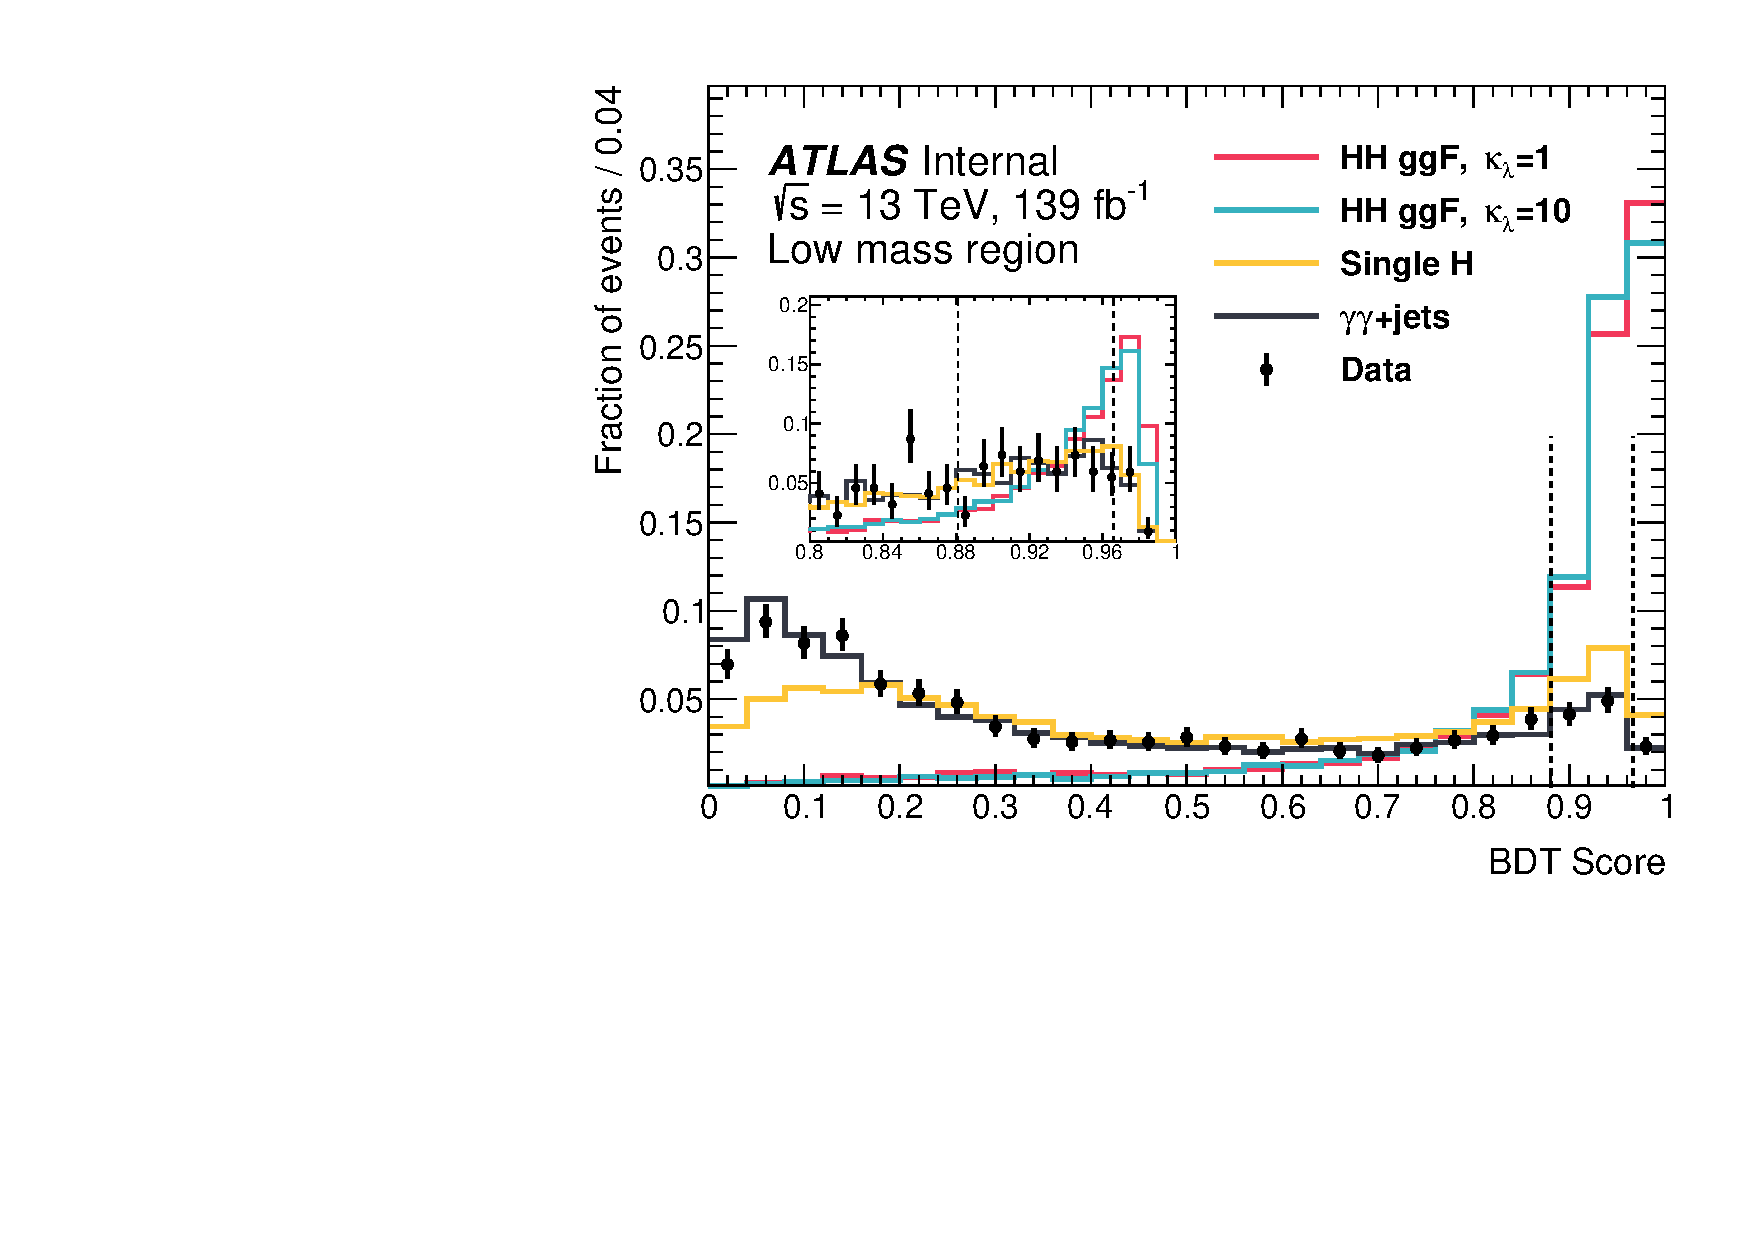
\includegraphics[width=.45\textwidth]{Ch5/Img/BDT_lowMass_Score.pdf} }
	\subfloat[High mass region][High mass region]{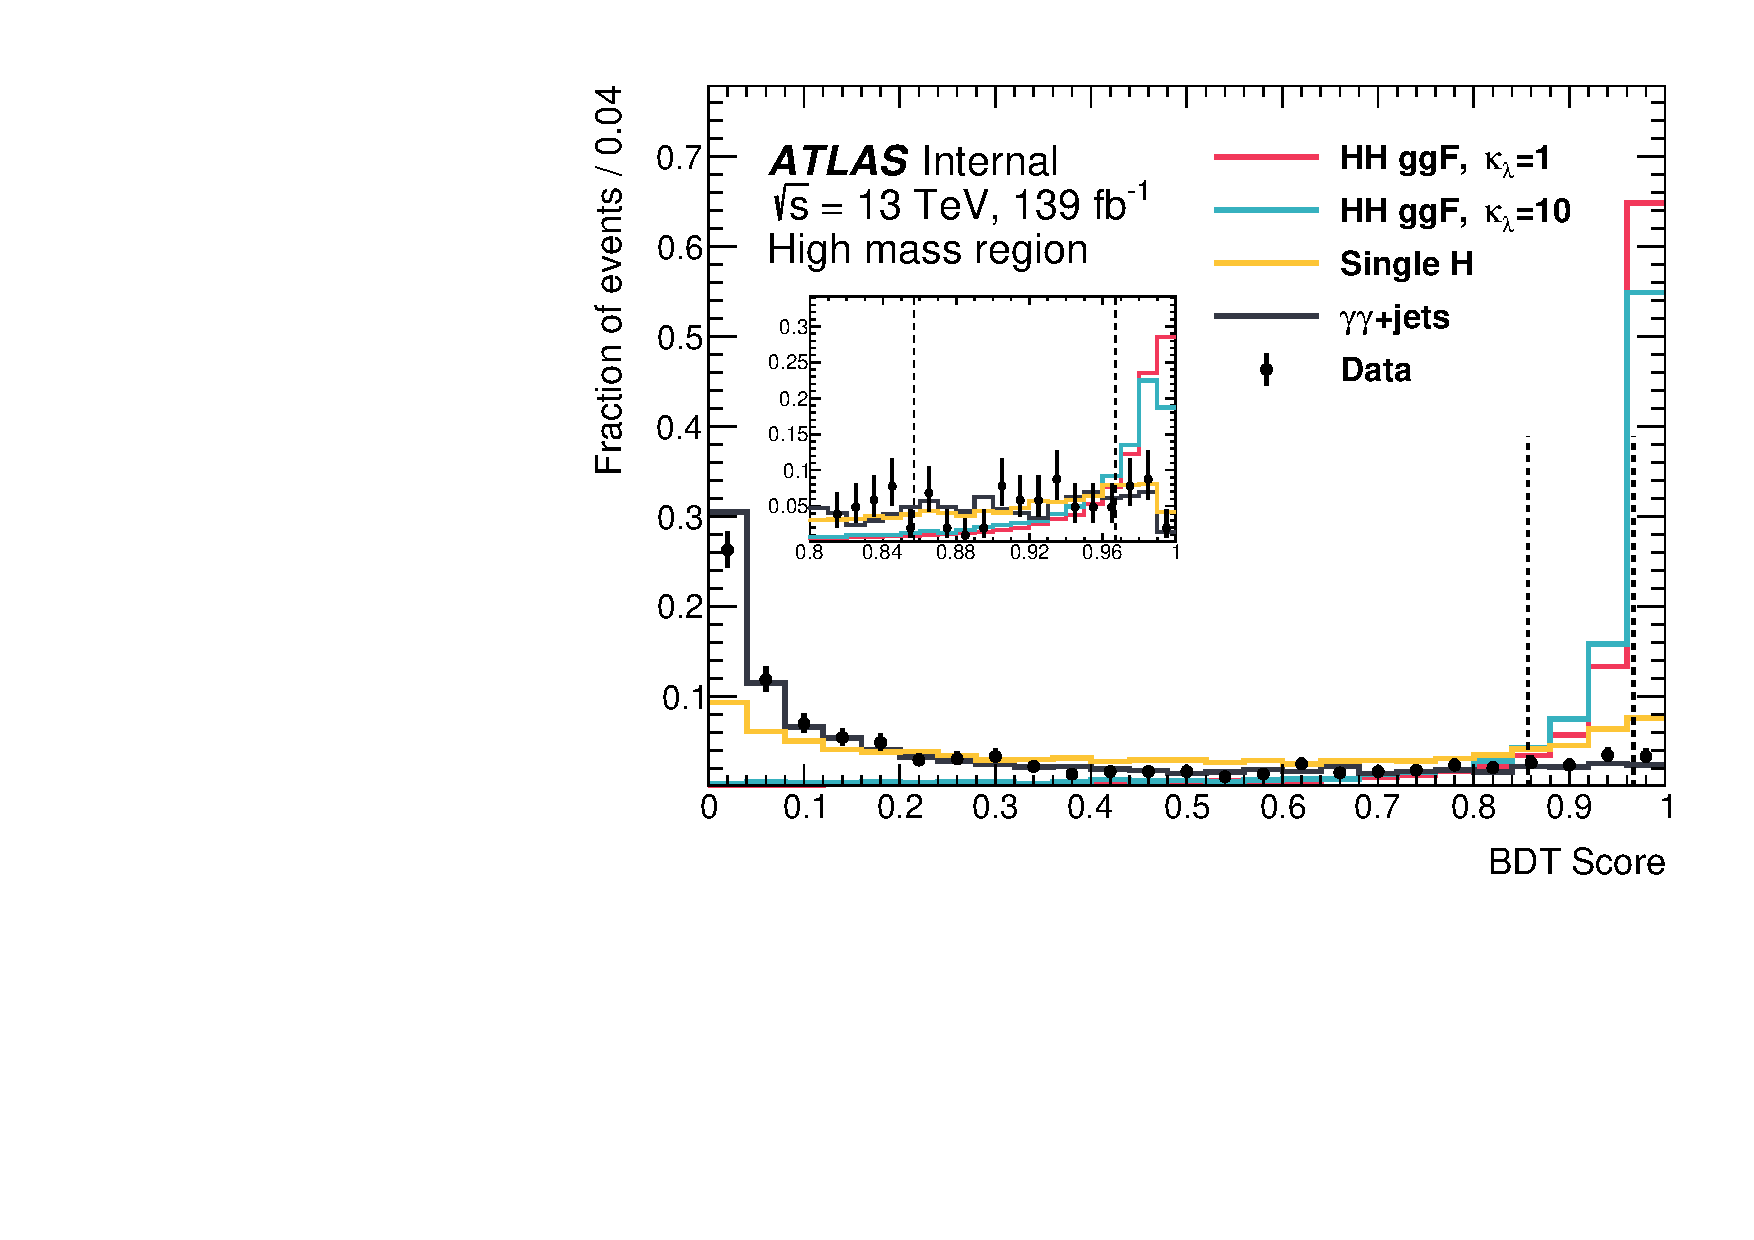
\includegraphics[width=.45\textwidth]{Ch5/Img/BDT_highMass_Score.pdf}} 
    \caption{The BDT score for the benchmark signals and the main backgrounds in the low- (a) and high- (b) mass categories. Distributions are normalized to unit area. The dotted lines denote the category boundaries. Events with a BDT score below 0.881 in the low mass region or below 0.857 in the high mass region are rejected.}
    \label{fig:HHyybb:ObjEvt:Evt:dBDT}
\end{figure}

\begin{table}[htbp]
    \centering
    \begin{tabular}{lc}
    \hline\hline
        Category & Selection criteria \\
    \hline
    High mass BDT tight & $m_{b \bar{b} \gamma \gamma}^{*} \geq$ 350 GeV, BDT score $\in$ [0.967, 1] \\
    High mass BDT loose & $m_{b \bar{b} \gamma \gamma}^{*} \geq$ 350 GeV, BDT score $\in$ [0.857, 0.967] \\
    Low mass BDT tight & $m_{b \bar{b} \gamma \gamma}^{*} <$ 350 GeV, BDT score $\in$ [0.966, 1] \\
    Low mass BDT loose & $m_{b \bar{b} \gamma \gamma}^{*} <$ 350 GeV, BDT score $\in$ [0.881, 0.966] \\
     \hline\hline
    \end{tabular}
    \caption{Definition of the analysis categories.}
    \label{tab:HHyybb:ObjEvt:Evt:Cat}
\end{table}
The BDT approach improves the analysis significance by approximately 20\% compared to the previous cut-based selection used in the 36 \ifb analysis \cite{yybb_36ifb}. The \myy distribution in each of the BDT categories are shown in Figure \ref{fig:HHyybb:ObjEvt:myy}. \\ 
\begin{figure}[htbp]
    \centering
    \subfloat[][High mass, BDT tight]{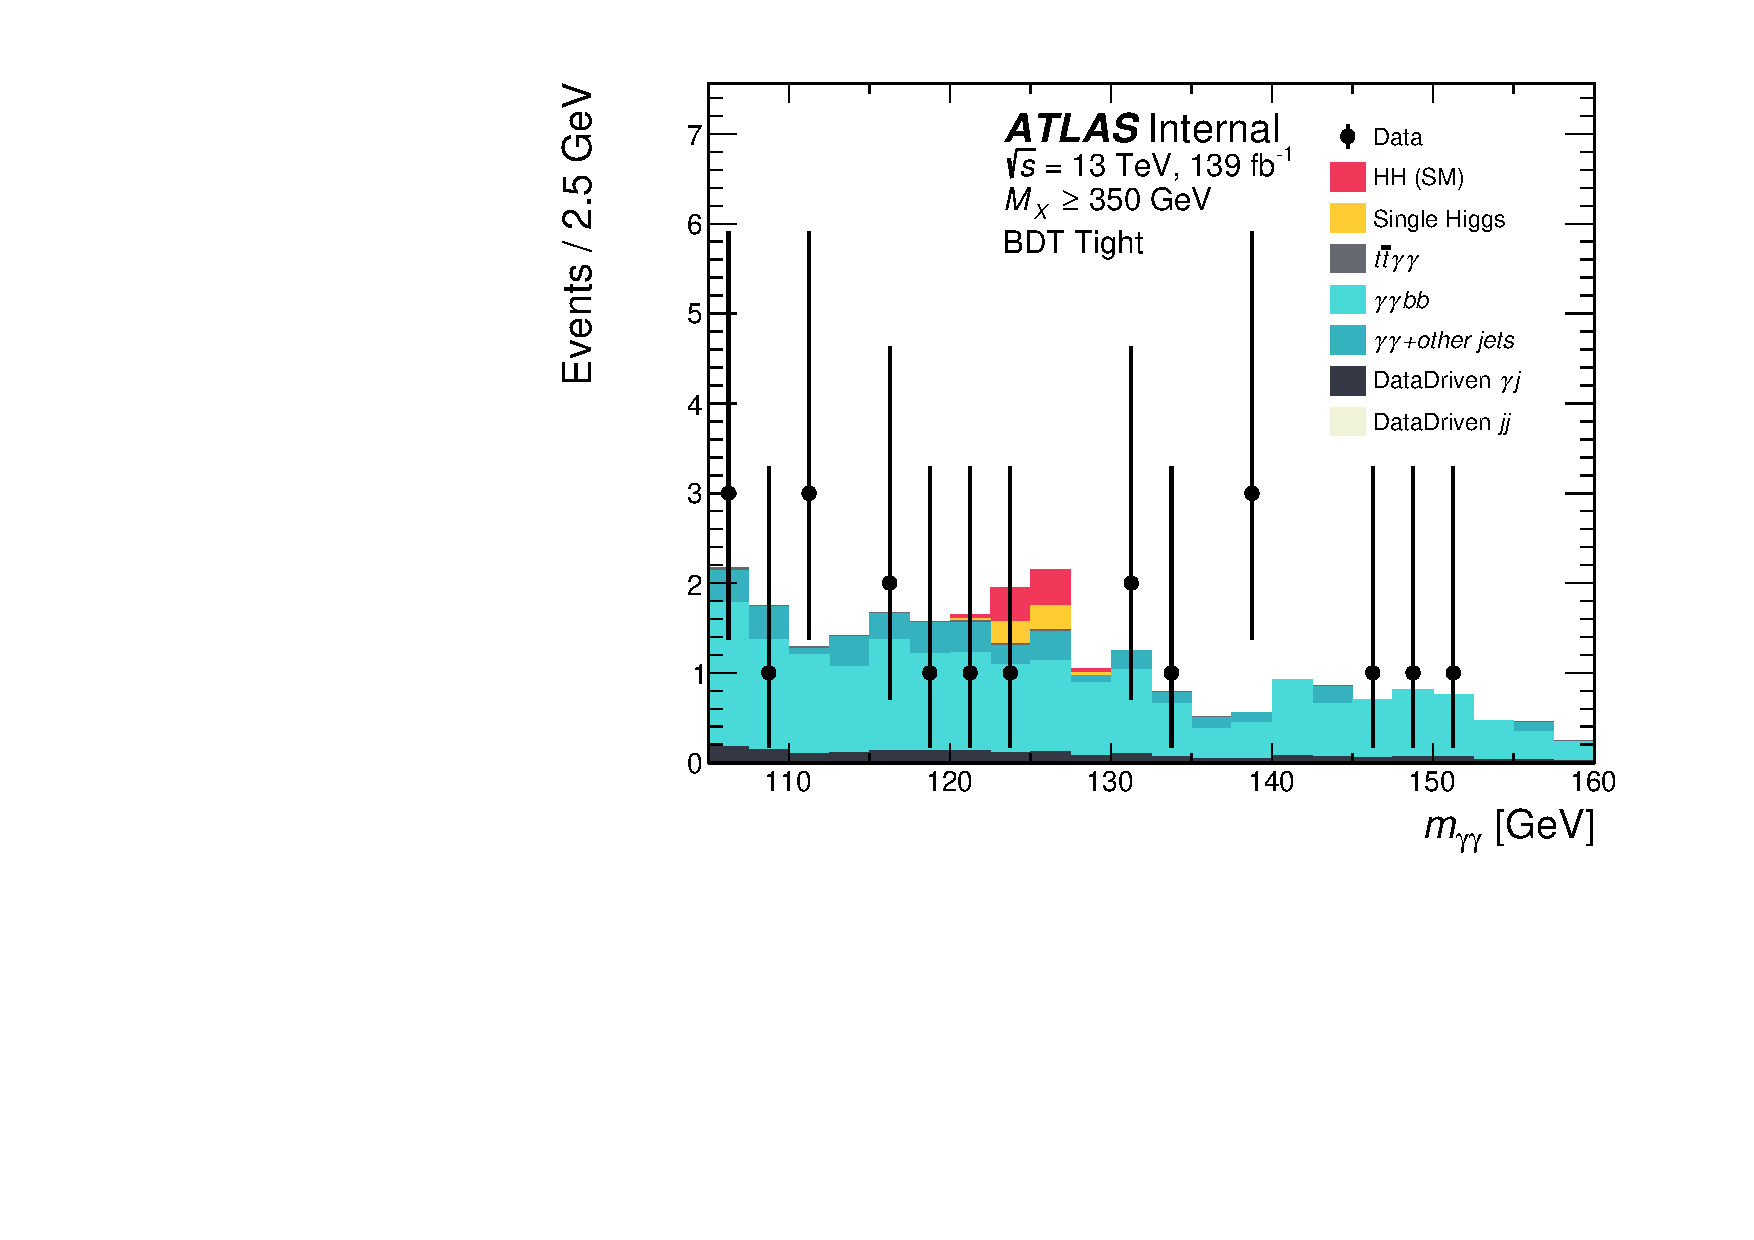
\includegraphics[width=.5\textwidth]{Ch5/Img/m_yy_XGBoost_btag77_withTop_BCal_tightScore_HMass.pdf}}
    \subfloat[][Low mass, BDT tight ]{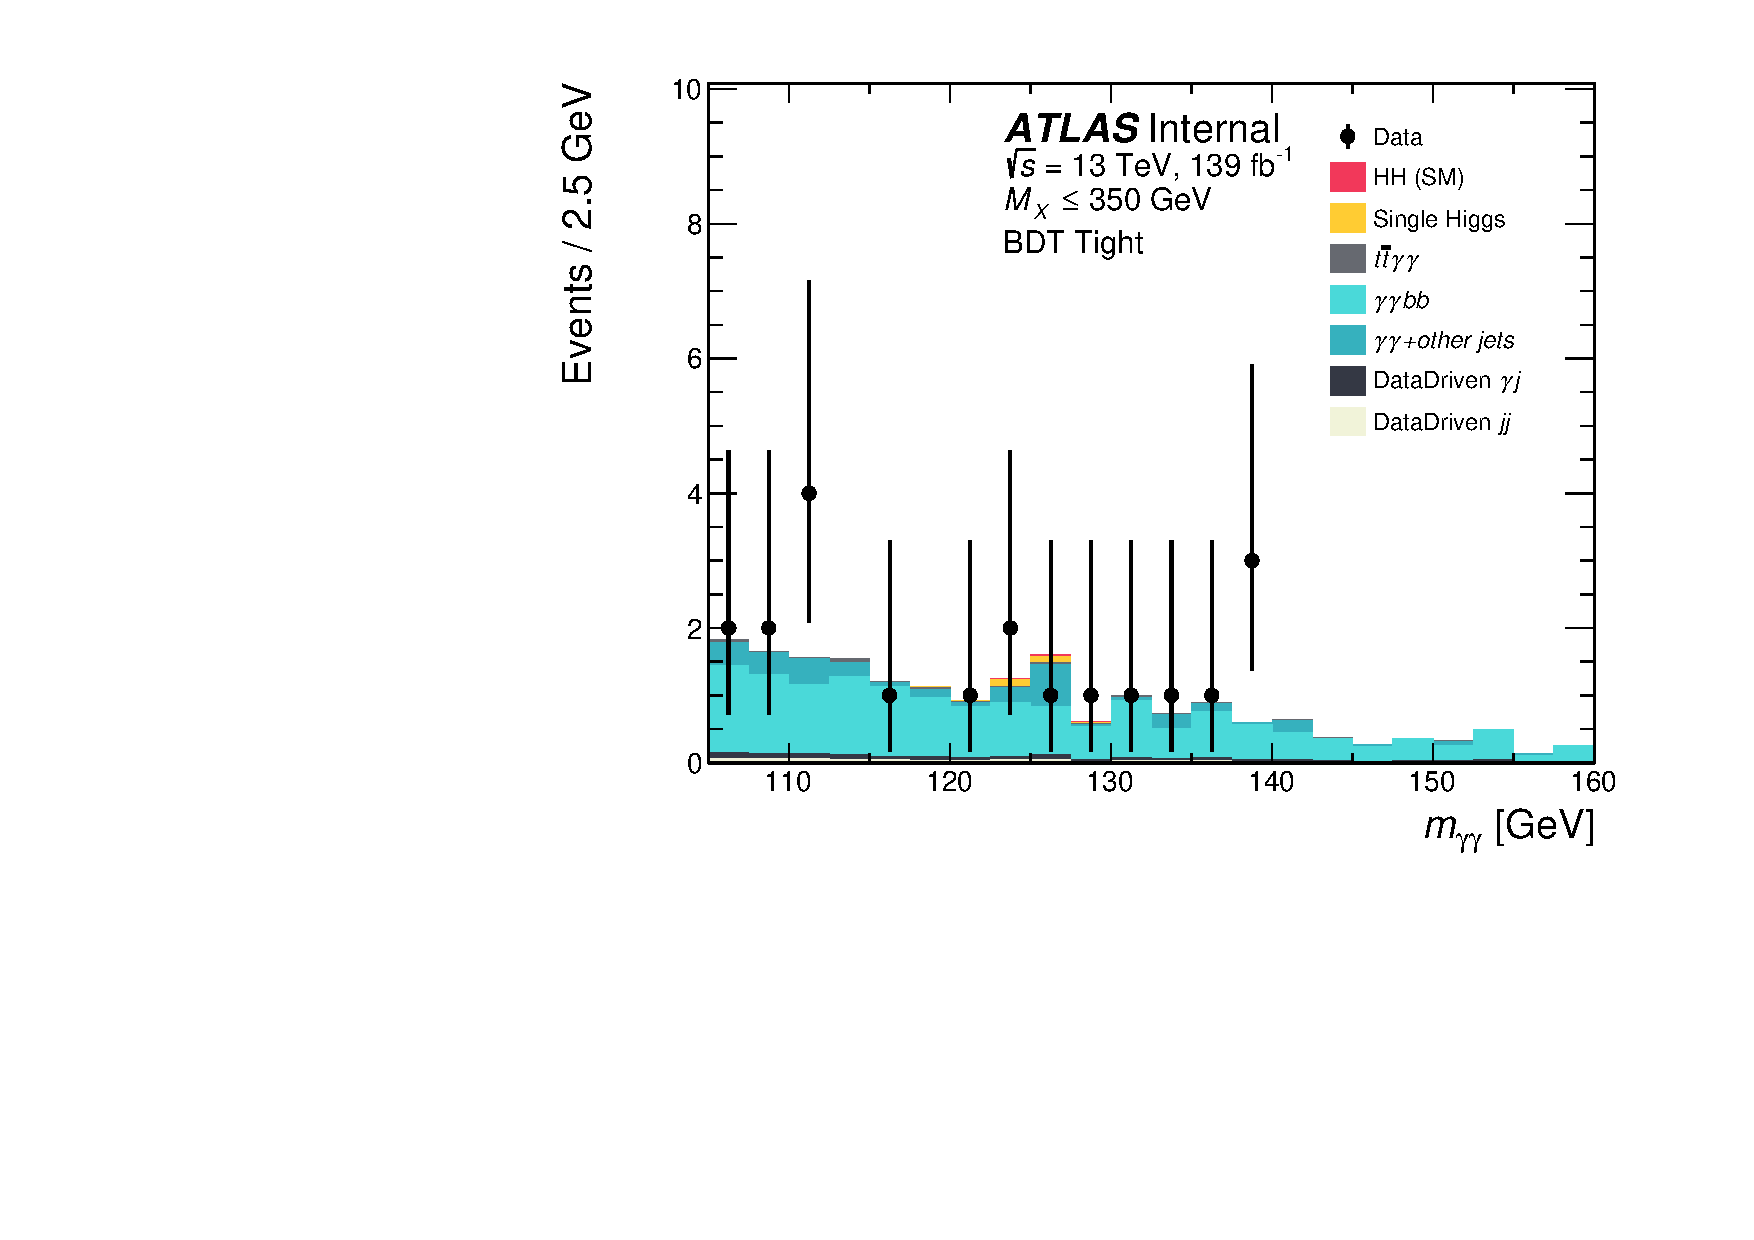
\includegraphics[width=.5\textwidth]{Ch5/Img/m_yy_XGBoost_btag77_withTop_BCal_tightScore_LMass.pdf}} \\
    \subfloat[][High mass, BDT loose]{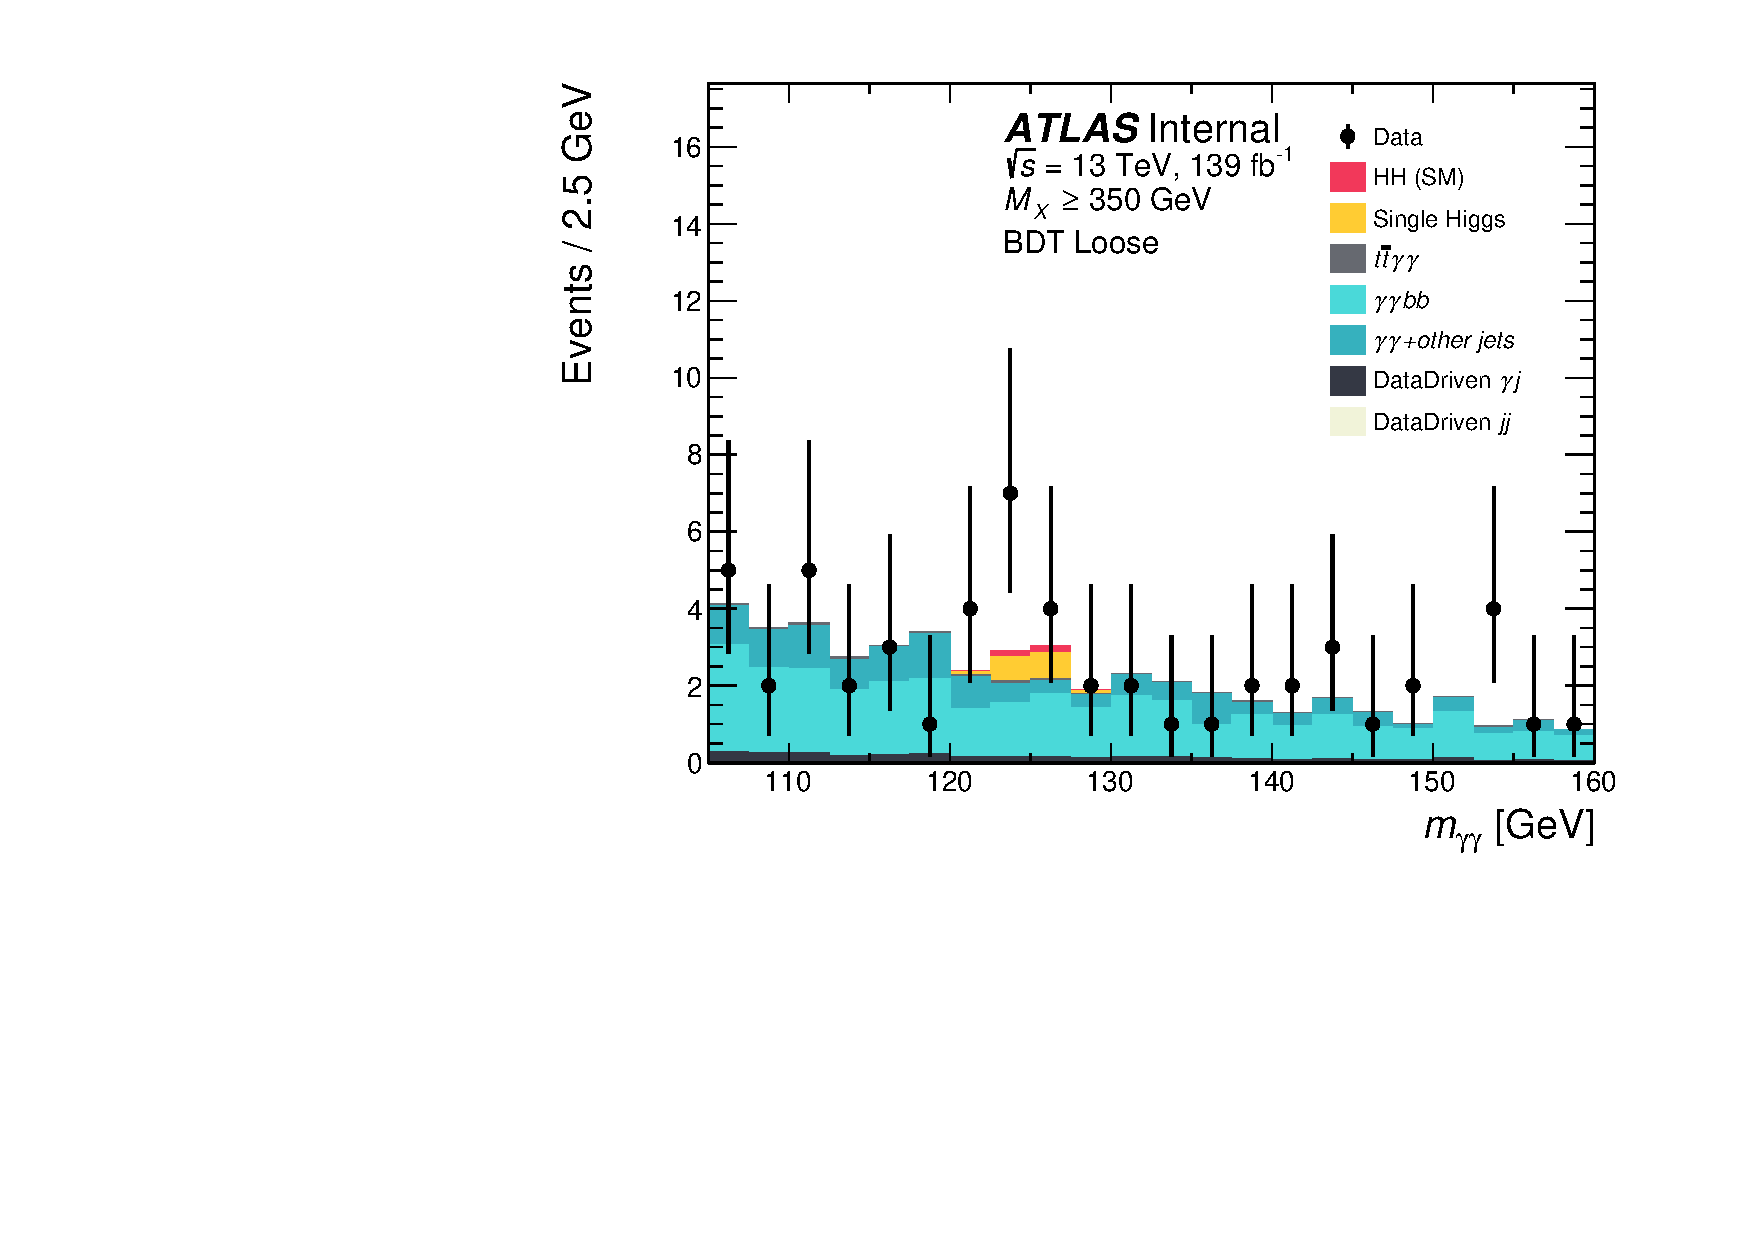
\includegraphics[width=.5\textwidth]{Ch5/Img/m_yy_XGBoost_btag77_withTop_BCal_looseScore_HMass.pdf}}
    \subfloat[][Low mass, BDT loose ]{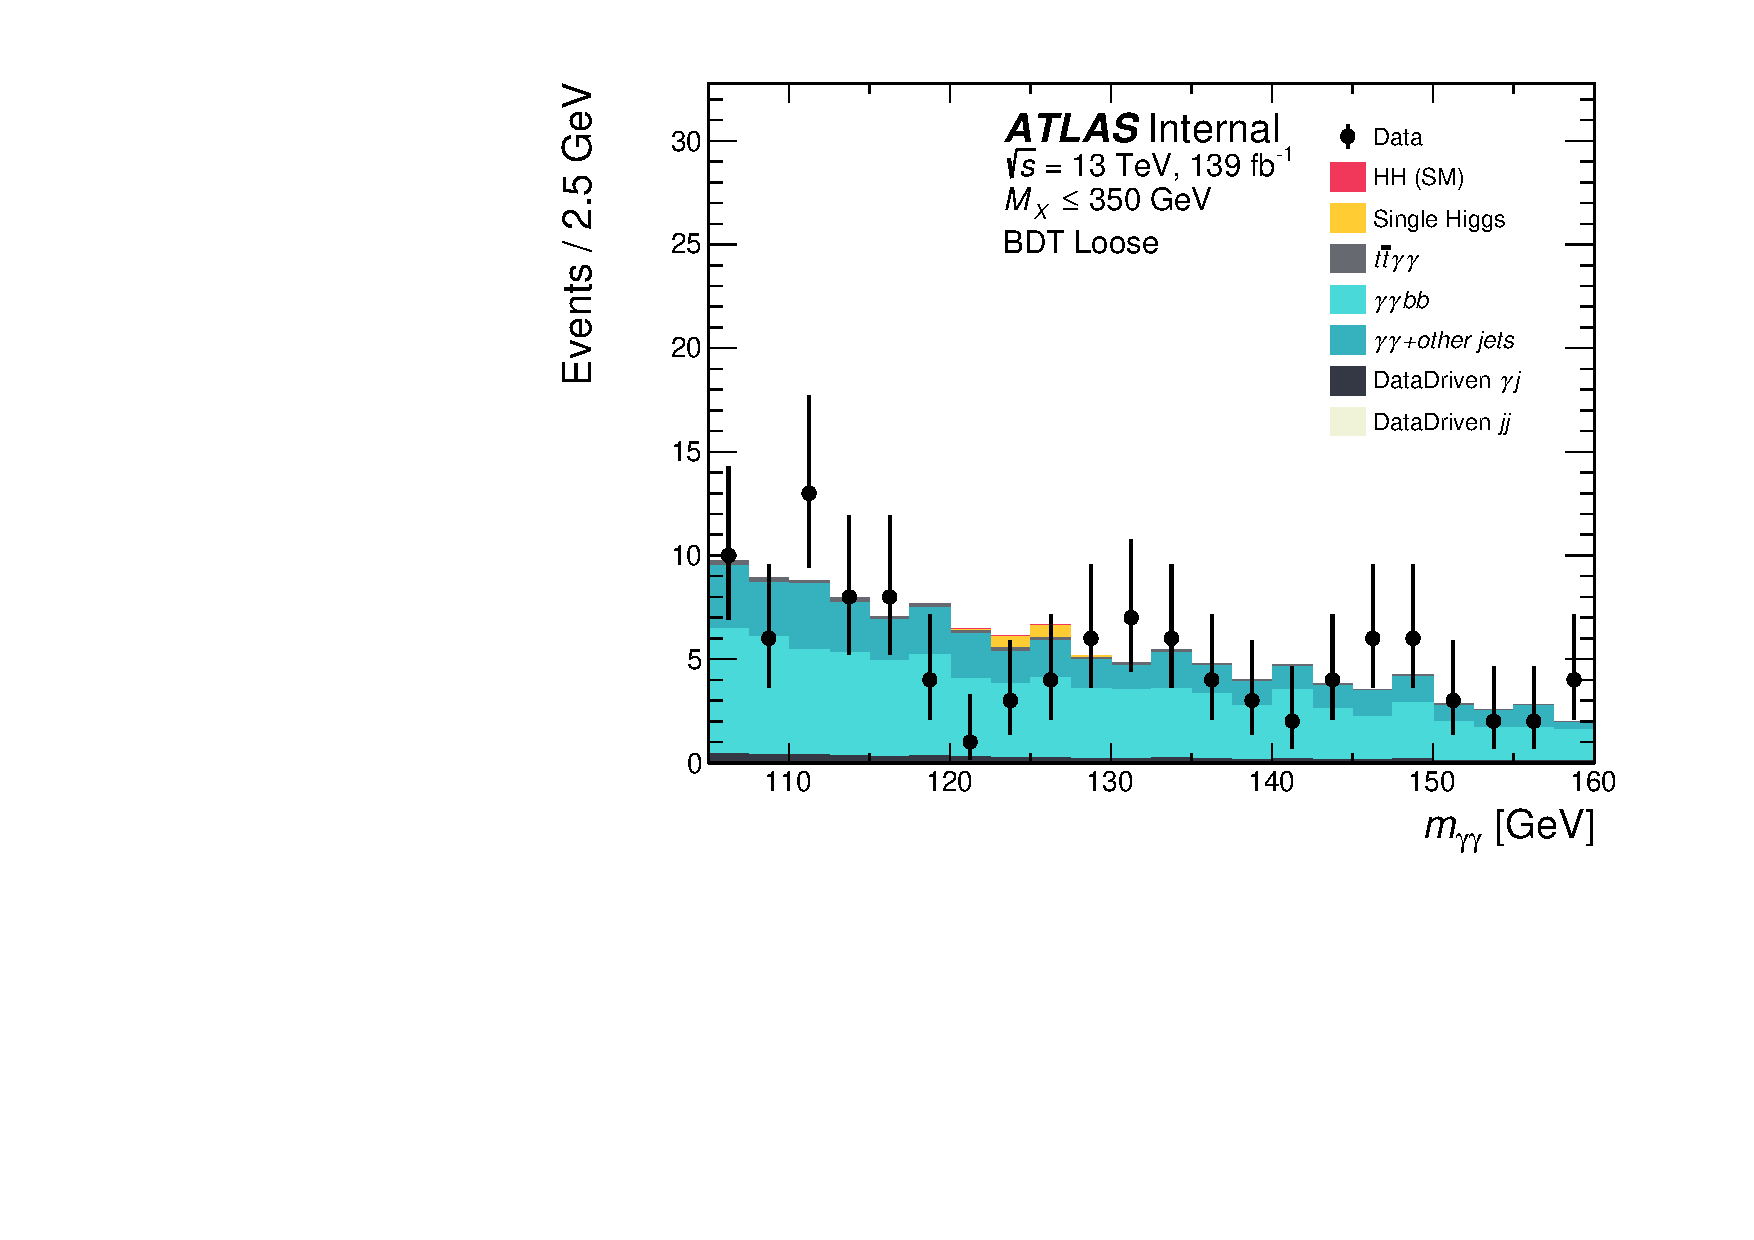
\includegraphics[width=.5\textwidth]{Ch5/Img/m_yy_XGBoost_btag77_withTop_BCal_looseScore_LMass.pdf}}
  
    \caption{Distributions of \myy in all signal categories. The simulated continuum background is scaled by the $\gamma\gamma$, $\gamma$-jet/jet-$\gamma$, and jet-jet fractions and normalized to the data side-band. The background decomposition is described in Section \ref{HHyybb:Modelling:Bkg}.}
    \label{fig:HHyybb:ObjEvt:myy}
\end{figure}


\subsection{Event selection using Deep Neural Network}
\label{HHyybb:ObjEvt:DNN}

The BDT categorization is used as baseline for the publication. In parallel, I developed a multi-label classification based on a Deep Neural Network (DNN) to classify events, and shows similar performance to the BDT. 
\subsubsection{Multi-label classification DNN}
Following the same strategy as the BDT, a potential gain can be achieved using a multi-label classification DNN. DNNs usually show a better handling of correlations between variables to enhance classifier performance. The multi-label classification attempts to classify each event in four process categories (HH signal, ZH, $t\bar{t}$H or continuum $\gamma\gamma$+jets). This helps in learning event topology for a better separation between signal and each background component separately. In addition, the multi-label classification allows for a control region where ZH is dominant, which could be used as a validation for the \HHyybb analysis. \\

A separate DNN classifier is trained in each mass region using the same signal and background definitions as the BDT. The architecture of the two classifiers is identical. The classifiers are built using the \textsc{Keras} library with \textsc{TensorFlow} as a backend \cite{keras,tensorflow}. It contains an input layer constructed from a batch normalization and a fully connected layer. Then five fully connected hidden layers with each one is followed with a dropout layer, and finally an output layer. Each of the fully connected layers has 128 nodes using a Rectified Linear Unit (ReLU) activation function, and their weights are randomly initialized by sampling from a truncated distribution centred on zero with width given by $\sqrt{\frac{2}{N_{inputs}}}$ where $N_{inputs}$ is the number of input features. The dropout layers are used to improve the robustness of the training and reduce overfitting effects. For the high mass region, the dropout rate is 11\%, while for the low mass region, the dropout rate is 22.5\%. The batch normalization layer is used to standardize the inputs to the first layer. The output layer is 4-node wide and activated using a softmax function which allows one to interpret the output as the probabilities for each associated class (ggF HH, ZH, $t\bar{t}$H or $\gamma\gamma$+jets) for the input event. During the training, a weighted categorical cross-entropy is used as loss function and the Adam optimizer for network weight optimization.\\
Weights of the loss function correspond to the event class weight computed as the weight of an event $j$ associated to class $i$ as:
\begin{equation}
    \text{weight}_i^j = \frac{N}{n\times N_{\text{class}_{i}}},
\end{equation}
where $n = 4$ is the number of classes, N is the total number of events and $N_{\text{class}_{i}}$ is the total number of events in the given class i. The event class weight enables the models to perform similarly between classes and reduces the issue of unbalanced data which affects the model classification ability.\\
The two DNN models are trained with a learning rate of $10^{-4}$ and a batch size fixed to 1000 events, with a maximum number of epochs set to 100. Similar to the CNN implemented for photon identification, an early stopping metric evaluated on the validation data sample throughout the training is imposed during the training phase. The early-stopping stops the training around epoch 40 to avoid overfitting.\\ 
DNNs use almost the same input variables as the BDT, as listed in Table \ref{tab:HHyybb:ObjEvt:Evt:BDT}, except for the single topness, $H_T$, the missing transverse energy and its azimuthal angle variables which are not included. The class-invariant symmetries (detector symmetry) complexity is removed by rotating all events around the beam axis in such a way that the leading photon has $\phi=0$. \\
Figure \ref{fig:HHyybb:ObjEvt:DNN:Loss} shows the evaluation of the loss function during the training time for the training and validation dataset.  The low mass model shows a high loss error compared to the model trained in the high mass region, which translates the signal like background distribution, reducing the model separation in the low mass region. \\
\begin{figure}[htbp]
    \centering
    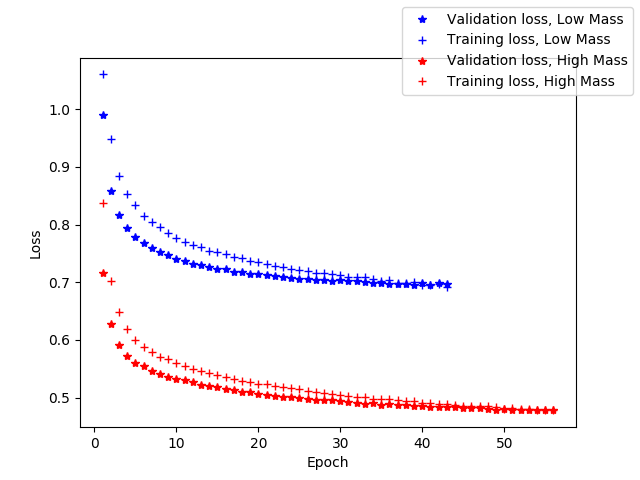
\includegraphics[width=0.45\textwidth]{Ch5/Img/Loss_DNN.png}
    \begin{tcolorbox}[colback=black!5!white,colframe=white!75!black]
    \caption{Evaluation of the loss function for high mass (red) and low mass (blue) DNNs as a function of epoch number.}
    \label{fig:HHyybb:ObjEvt:DNN:Loss}
    \end{tcolorbox}
    
\end{figure}
\\
One of the performance measurement of a classifier is the confusion matrix: the matrix compares the actual target values with those predicted by the model. This gives a holistic view of the performance of the classification model as well as the associated errors. Figure \ref{fig:HHyybb:ObjEvt:DNN:CM} shows the confusion matrix for high mass and low mass models. Note that the threshold value for the prediction of the model is set to 0.5 on the softmax outputs. Both models show a high ($\sim$19\%) confusion between the ggF HH signal and the ZH background, coming from the similarity between the event topology of the two processes. In the low mass region, the performance clearly decreases due to the similarity in the kinematics and event topology between ggF HH and backgrounds which degrades the sensitivity at high \kl values.
\begin{figure}[htbp]
    \centering
    \subfloat[][]{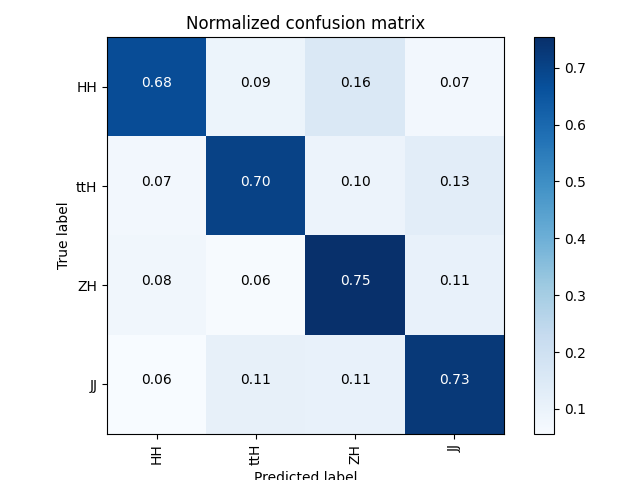
\includegraphics[width=.45\textwidth]{Ch5/Img/cm_SM.png}}
    \subfloat[][]{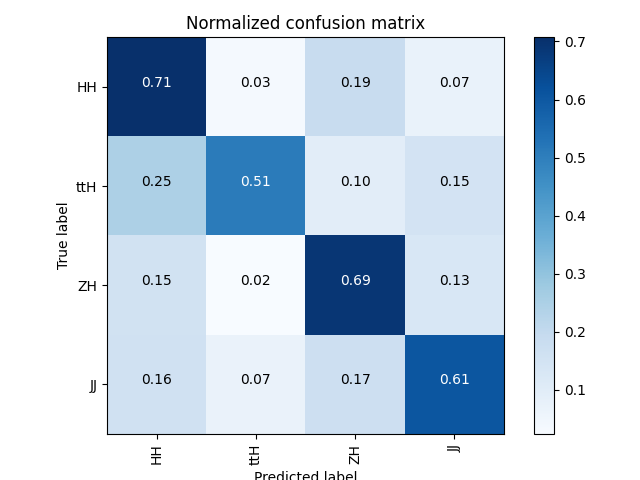
\includegraphics[width=.45\textwidth]{Ch5/Img/cm_BSM.png}}
    \begin{tcolorbox}[colback=black!5!white,colframe=white!75!black]
    \caption{Normalized (to unity) confusion matrix for (a) high mass and (b) low mass models. JJ here denote the continuum $\gamma\gamma+$jets.}
    \label{fig:HHyybb:ObjEvt:DNN:CM}
    \end{tcolorbox}
    
\end{figure}

\subsubsection{Discriminant variable}
The four outputs of the softmax layer are combined in a single discriminant denoted $d_{HH}$ for each region, the probabilities are normalized to the corresponding process cross-section.
\begin{equation}
    d_{HH}^{HM} = \log \left(\frac{\sigma_{SM}.p_{HH}}{\sigma_{ZH}.p_{ZH}+\sigma_{t\bar{t}H}.p_{t\bar{t}H}+\sigma_{\gamma\gamma+jets}.p_{\gamma\gamma+jets}}\right)
    \label{eq:DHH_HM}
\end{equation}
\begin{equation}
    d_{HH}^{LM} = \log \left(\frac{\sigma_{\kappa_\lambda10}.p_{HH}}{\sigma_{ZH}.p_{ZH}+\sigma_{t\bar{t}H}.p_{t\bar{t}H}+\sigma_{\gamma\gamma+jets}.p_{\gamma\gamma+jets}}\right)
    \label{eq:DHH_LM}
\end{equation}
$d_{HH}^{HM}$ in Eq. \ref{eq:DHH_HM} represents the $d_{HH}$ discriminant for the high mass region, while Eq. \ref{eq:DHH_LM} is the $d_{HH}$ discriminant in the low mass region. \\
Figure \ref{fig:HHyybb:ObjEvt:DNN:dHH} shows the distribution of $d_{HH}$ discriminant for each process (ggF HH, ZH, $t\bar{t}$H and $\gamma\gamma$+jets) in each region. At high mass, $d_{HH}$ shows a clear separation between the HH and other processes, while for low mass the discrepancy is low as expected. The side-band data follows the continuum background closely, indicating a good modelling of the $d_{HH}$ distribution. 
\begin{figure}[htbp]
    \centering
    \subfloat[$d_{HH}^{HM}$][$d_{HH}^{HM}$]{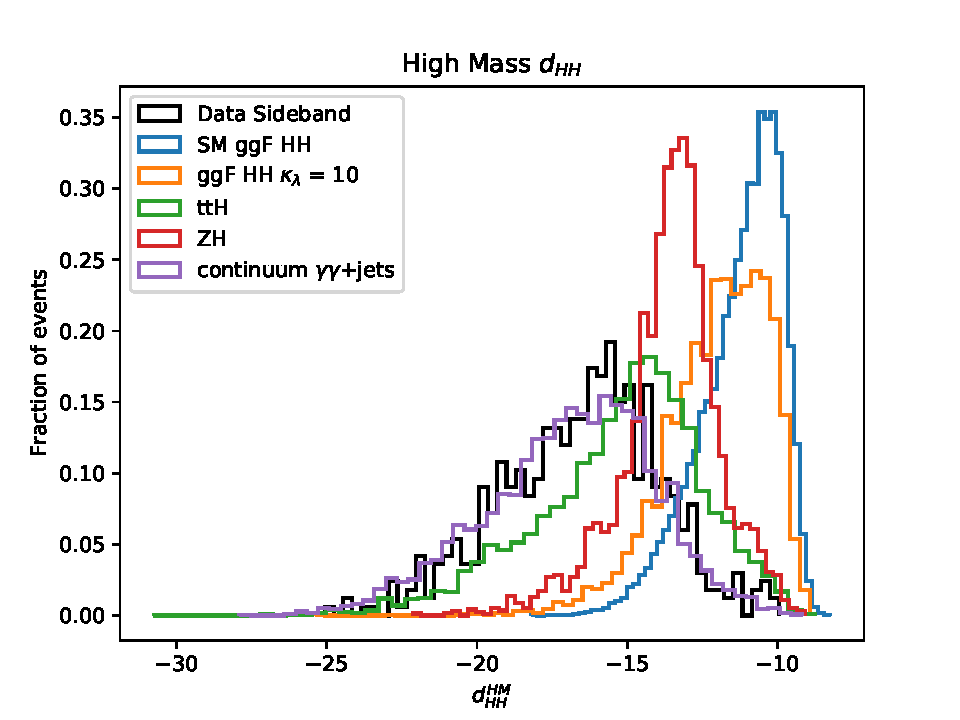
\includegraphics[width=.45\textwidth]{Ch5/Img/dHH_SM.pdf}}
    \subfloat[$d_{HH}^{LM}$][$d_{HH}^{LM}$]{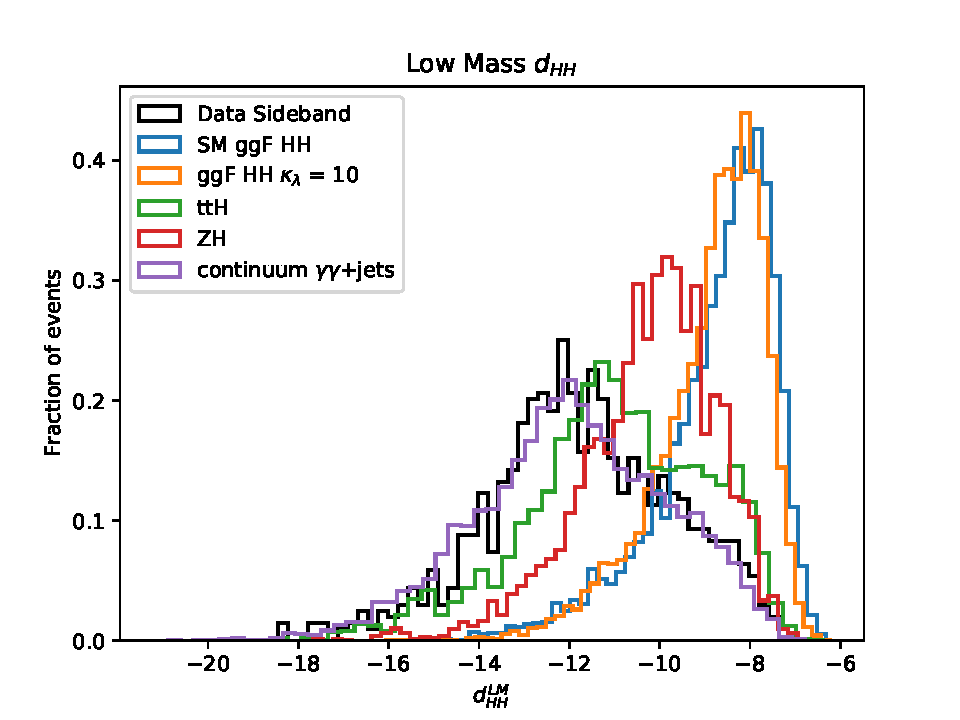
\includegraphics[width=.45\textwidth]{Ch5/Img/dHH_BSM.pdf}}
    \begin{tcolorbox}[colback=black!5!white,colframe=white!75!black]
    \caption{$d_{HH}$ discriminant distribution in (a) high mass and (b) low mass. The black line shows the real data in the sideband region ($m_{\gamma\gamma}\in[105,120] \cup [130,160]$).}
    \label{fig:HHyybb:ObjEvt:DNN:dHH}
    \end{tcolorbox}
    
\end{figure}

\subsubsection{Significance scan}
In each mass region, the corresponding discriminant is scanned after applying 90 $<$ \mbb $<$ 140 GeV requirement to build two orthogonal categories high $d_{HH}$ and low $d_{HH}$ with a maximum significance. The category with the highest significance must have at least 0.8 continuum $\gamma\gamma$+jets events in the $123<m_{\gamma\gamma}<127$ GeV mass range sufficient to perform reliable \myy fit. This is done similarly to the BDT. The significance is computed using the Asimov formula \cite{Z} defined as: 
\begin{equation}
    Z = \sqrt{2\left[(s+b)\times log(1+s/b)-s\right]},
\end{equation}

where, $s$ is the ggF HH signal yield and $b$ is the total background yield. \\
In total, four categories are defined, two for the low mass region and two for the high mass region. The significances of the four categories are then combined for the final significance. Table \ref{tab:Sig} lists the significance in each category.
\begin{table}[htbp]
    \centering
    \begin{tabular}{lcc}
        \hline\hline
        Categories & SM ggF HH & BSM $\kappa_\lambda$=10 ggF HH \\
        \hline
        High mass, High $d_{HH}$ & 0.53 & 2.45 \\
        High mass, Low $d_{HH}$ & 0.11 & 0.94 \\
        Low mass, High $d_{HH}$ & 0.03 & 2.21 \\
        Low mass, Low $d_{HH}$ & 0.01 & 0.54 \\
        \hline
        Combined & 0.54$\sigma$ & 3.47$\sigma$ \\
        \hline
        \hline
    \end{tabular}
    \begin{tcolorbox}[colback=black!5!white, colframe=white!75!black]
    \caption{Significance in each category for SM ggF HH and BSM $\kappa_\lambda$ = 10 ggF signals.}
    \label{tab:Sig}
    \end{tcolorbox}
    
\end{table}
\\
The proposed selection based on a DNN shows similar performances with respect to the BDT with less inputs variables. The missing variables in the DNN are very discriminant in the BDT case, thus including those variables in the DNN could have enhanced the DNN performance. Given the timescale of the analysis, the DNN work was stopped here to focus on work with higher priority. Future DNN optimization are kept for the Run-3 analysis. The DNN based selection is available and documented for the next publication with Run-3 data. \\

\section{Signal and background modelling}
\label{HHyybb:Modelling}

To extract the \HHyybb signal yield, a fit to the \myy distribution in the range [105, 160] GeV is performed in the data. Analytical functions are used to describe the signal, single Higgs boson and the continuum backgrounds. Parameters of the signal and the peaking single Higgs boson background shapes are fixed on simulated distributions.

\subsection{Signal and single Higgs boson parameterization}
\label{HHyybb:Modelling:Sig}

Both signal and peaking single Higgs boson backgrounds are described analytically by a Double-Sided Crystal Ball (DSCB) function which is characterized by a Gaussian core and asymmetric power law tails \cite{Higgs_2018}, defined as:

\begin{equation}
    f_{\mathrm{DSCB}}\left(m_{\gamma \gamma}\right)=N \times\left\{\begin{array}{ll}
e^{-t^{2} / 2} &  if \ -\alpha_{low } \leq t \leq \alpha_{high } \\

\frac{e^{-\frac{1}{2} \alpha_{low }^{2}}} {  \left[  \frac{1}{ R_{low} } \left(R_{low }-\alpha_{low }-t\right) \right]^{n_{low }}} & if \ t<-\alpha_{low } \\

\frac{e^{-\frac{1}{2} \alpha_{high }^{2}}} {  \left[  \frac{1}{ R_{high} } \left(R_{high }-\alpha_{high }-t\right) \right]^{n_{high }}} &  if \ t>\alpha_{high }
\end{array}\right.
\end{equation}
with $t = \frac{m_{\gamma\gamma} - \mu_{CB}}{\sigma_{CB}}$. $\mu_{CB}$ and $\sigma_{CB}$ describe the mean and the width of the Gaussian core, $\alpha_{low/high}$ the transition from the core to the tails of the distribution and $n_{low/high}$ the tails. N normalizes the distribution. The explicit separation of the Gaussian core from the tails in this function allows an easy treatment of the systematic uncertainties, as the energy scale uncertainty impacts the mean $\mu_{CB}$ and the energy resolution systematic the width $\sigma_{CB}$.\\
The normalizations are obtained from the expected MC yields. For each BDT category, the parameters of the DSCB are obtained from a fit of the \myy distribution obtained from simulation of the ggF and VBF HH processes with \kl = 1, since no significant dependence of the functional form with \kl was found. \\
Fitted parameters are further allowed to vary only within the systematic uncertainties on the energy scale and resolution. Injection tests are performed to quantify potential biases from the signal HH only fit and signal + single Higgs boson fit. No statistically significant bias ($<$ 10\%) was observed in both tests, thus the same parameterized functions are used to fit the signal and single Higgs boson backgrounds.    

\subsection{Continuum background parameterization}
\label{HHyybb:Modelling:Bkg}

The continuum background estimation is done in a data-driven way. The simulated $\gamma\gamma$+jets sample is used only to select the functional form and its parameters are then left completely free in the fit to the data, reducing uncertainties due to background mismodelling. The background is decomposed into several components to take into account contribution from the continuous $\gamma\gamma$, $\gamma$-jet ($\gamma j$) and jet-jet ($jj$) fake photons components. The decomposition is done using a 2x2 ABCD side-band method \cite{ABCD}, in which an equation system is built and then solved to determine the relative contribution of each component (purity). The purities are measured inclusively and in each BDT category. Inclusively, the $\gamma\gamma$ event purity is found to be 85 $\pm$ 2.9\% and the remaining 15 $\pm$ 2.8\% consists of $\gamma j$ events and a negligible amount of $jj$ events. The $\gamma\gamma$ contribution increases after the BDT selection since the BDT tends to select events with higher photon \pT, thus more real photons. The decomposition is shown in Figure \ref{fig:HHyybb:Modelling:Bkg:Decom}. 
\begin{figure}[htbp]
    \centering
    \subfloat[][]{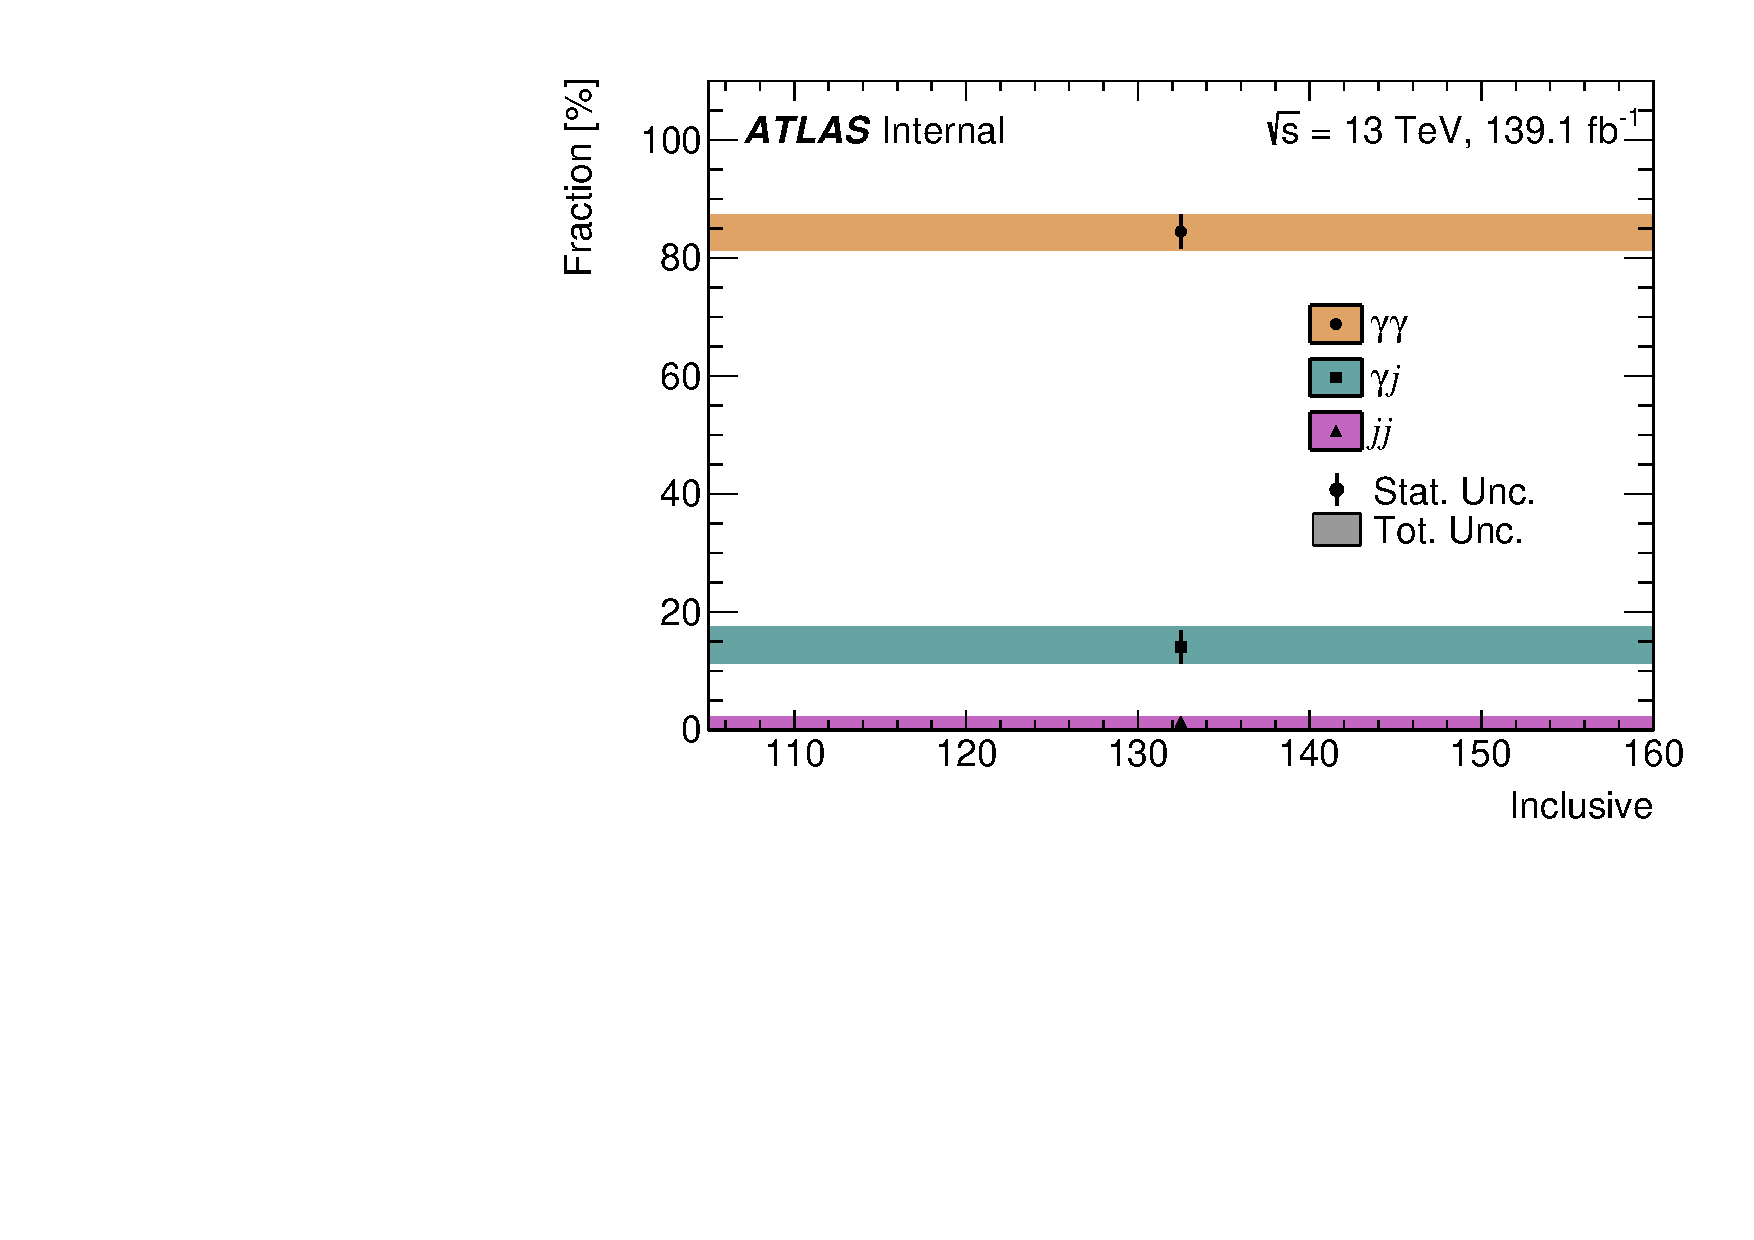
\includegraphics[width=.5\textwidth]{Ch5/Img/figures_BackgroundDecomposition_plot_purity_inclusive.pdf}}
    \subfloat[][]{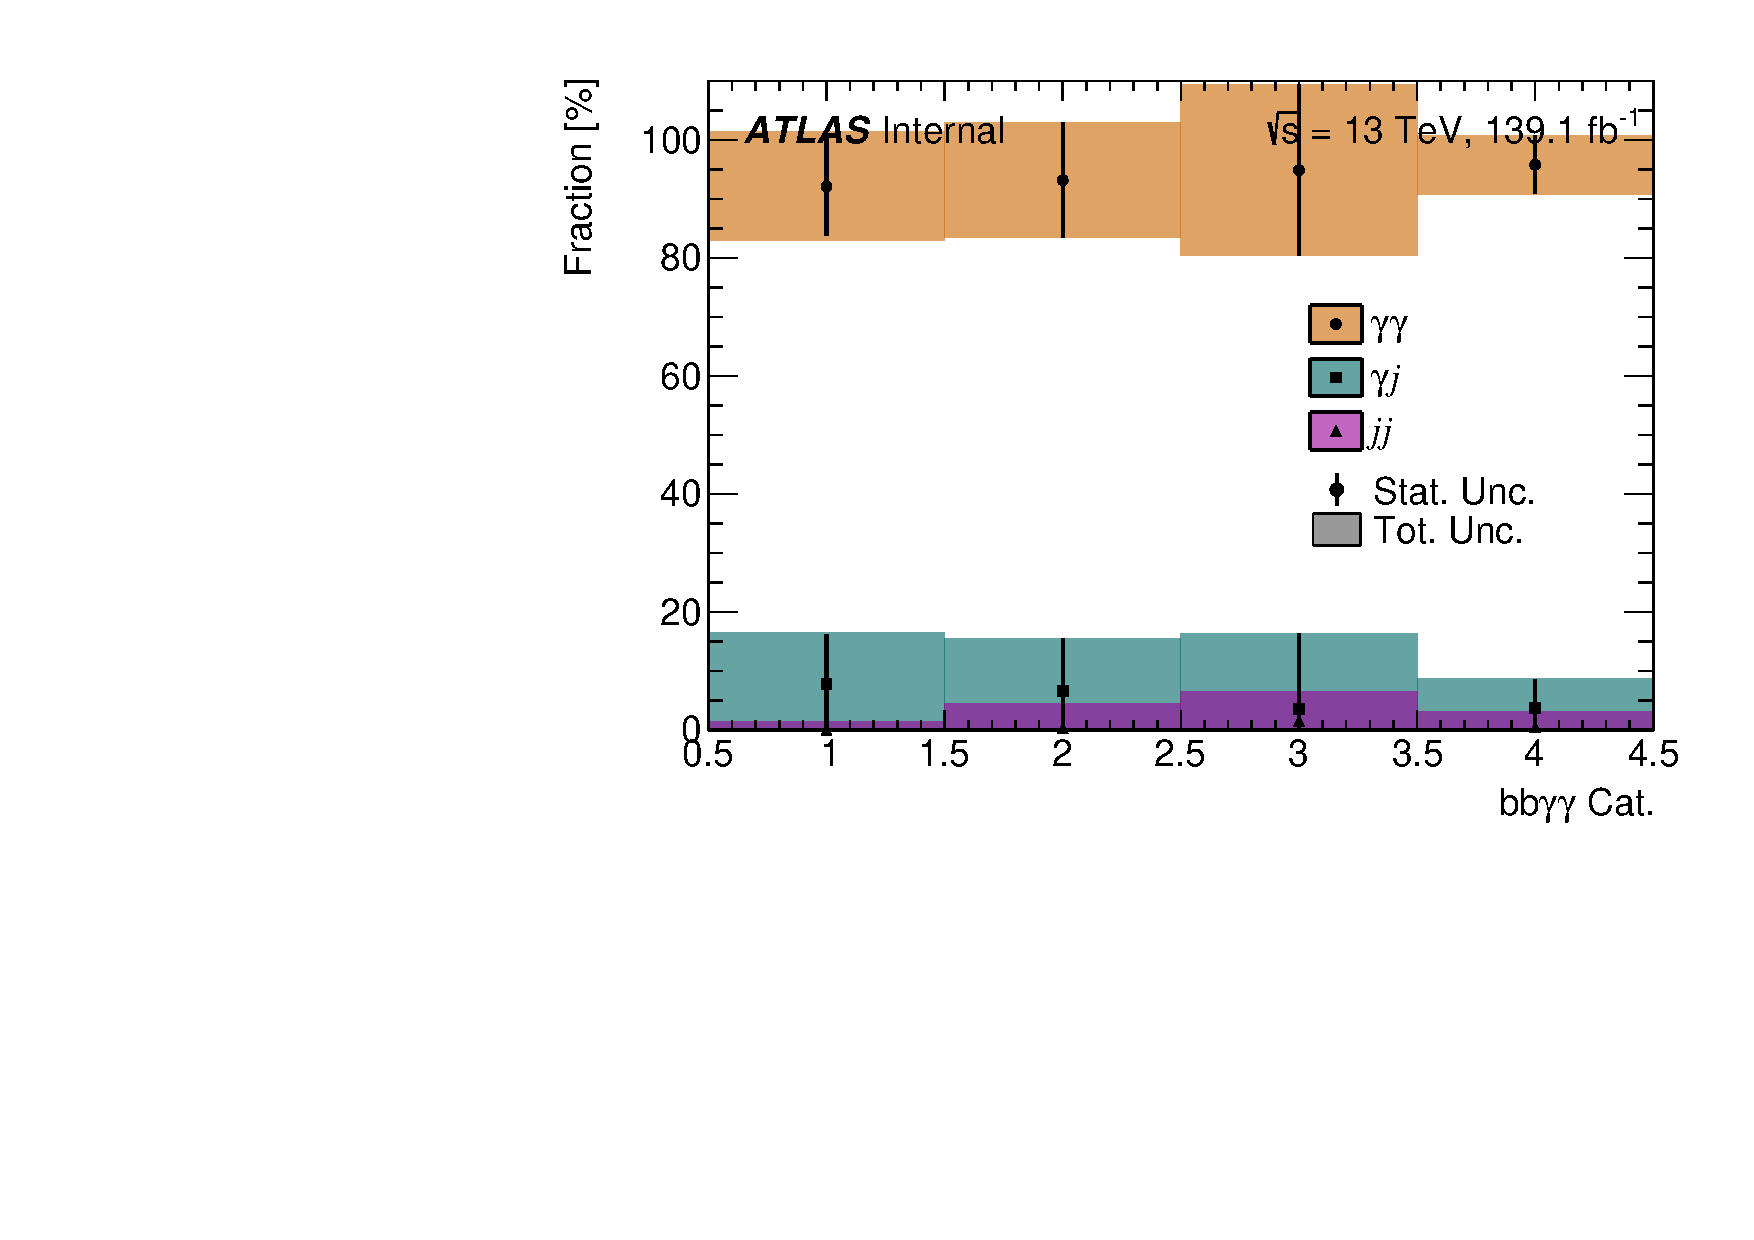
\includegraphics[width=.5\textwidth]{Ch5/Img/figures_BackgroundDecomposition_plot_purity_yybb_nonRes_XGBoost_btag77_BCal_Cat.pdf}}
    \caption{$\gamma\gamma$, $\gamma j$, and $jj$ fractions in the inclusive (a) and the BDT categories (b). In the BDT figure bin 1 corresponds to the High mass BDT tight category, bin 2 to the High mass BDT loose category, bin 3 to the Low mass BDT tight category, and finally bin 4 to the Low mass BDT loose category.}
    \label{fig:HHyybb:Modelling:Bkg:Decom}
\end{figure}
\\
The functional form is chosen by fitting the simulated background template. Given the high $\gamma\gamma$ purity, the template is constructed from the \texttt{SHERPA} $\gamma\gamma$+jets normalized to the data side-band. The bias on the specific choice of functional form (to absorb a potential signal or create an artificial signal) is determined by the spurious signal test. 

\subsubsection{Spurious signal test}
\label{HHyybb:Modelling:Bkg:SS}
The spurious signal (SS) refers to any potential fake signal $N_{SS}$ obtained from fitting a smooth background only distribution to a function that describes the signal plus background shape. The $N_{SS}$ is taken to be the largest number of fitted signal events computed for Higgs boson masses varying in intervals of 1 GeV from 121 to 129 GeV. The SS requires the tested function to fulfil the following criteria: 
\begin{itemize}
    \item $N_{SS} < $ 10\% $N_{s}^{exp}$, where $N_{s}^{exp}$ is the expected number of signal events within the BDT category. 
    \item $N_{SS} < $ 20\% $\sigma_{bkg}$, where $\sigma_{bkg}$ is the statistical uncertainty on the fitted signal events when performing a signal+background fit to the template. 
\end{itemize}


Due to the limited background statistics, a new variable $\xi_{SS}$ is defined to relax the criterion defined before. The $\xi_{SS}$ is defined in a such way as to allow for a 2$\sigma$ local statistical fluctuation in the background template. $\xi_{SS}$ is defined as: 
\begin{equation}
    \zeta_{\mathrm{SS}}=\left\{\begin{array}{ll}
N_{\mathrm{SS}}+2 \Delta_{\mathrm{MC}}, & N_{\mathrm{SS}}+2 \Delta_{\mathrm{MC}}<0 \\
N_{\mathrm{SS}}-2 \Delta_{\mathrm{MC}}, & N_{\mathrm{SS}}-2 \Delta_{\mathrm{MC}}>0 \\
0, & \  otherwise 
\end{array}\right.
\end{equation}
where $\Delta_{MC}$ is the statistical uncertainty on $N_{SS}$ due to limited statistics. $\xi_{SS}$ should then pass the same criteria as $N_{SS}$. \\
The function that gives the smallest $N_{SS}$ is selected as the final background function and the $N_{SS}$ is added as a systematic on the signal yield. The exponential function "$\exp(a.m_{\gamma\gamma})$" is found to be the best choice for all BDT categories and the corresponding parameters for SS are shown in Table \ref{tab:HHyybb:Modelling:Bkg:SS}.

\begin{table}[]
    \centering
    \begin{tabular}{lccc}
    \hline\hline
       Category  & $N_{SS}$ & $Z_{sp}$ & p($\chi^2$) [\%] \\
       \hline
       High mass BDT tight &  0.688 & 0.394 & 68.8 \\
       High mass BDT loose &  0.990 & 0.384 & 30.5 \\
       Low mass BDT tight  &  0.594 & 0.378 & 29.8 \\
       Low mass BDT loose  & 1.088  & 0.272 & 26.9 \\
       \hline\hline
    \end{tabular}
    \caption{Spurious signal result for the exponential functional form for the various BDT categories. In each category, the spurious signal value, its ratio to the expected statistical error from data, and $\chi^2$ the probability of the background-only fit.}
    \label{tab:HHyybb:Modelling:Bkg:SS}
\end{table}

\section{Systematic uncertainties}
\label{HHyybb:Syst}
Due to the small number of expected signal events (Section \ref{chap1:HH:HPD}), and the restrictive event selection, the dominant source of uncertainty in this analysis is still the statistical one. Nevertheless, the amplitude of systematic sources have to be evaluated. They can be split into two categories: the experimental and theoretical uncertainties. The impact of each systematic on the shape and/or the expected event yield (Normalization) is evaluated in each BDT category. Since the continuum background is the main source of background, and is estimated with data-driven method, no associated systematic are assigned. Systematic are estimated for the single Higgs boson backgrounds and HH signal using simulation. Technically, these systematic uncertainties are implemented as nuisance parameters in the statistical model and constrained by a Gaussian or log-normal function in most cases. 
\subsubsection{Experimental systematic uncertainties}
\label{HHyybb:Syst:Exp}
Experimental systematic uncertainties are mostly related to the reconstruction, the calibration, the tagging and the identification of the physics objects used in the analysis. In addition to, a 1.7\% uncertainty on the integrated luminosity used in this analysis (full Run-2). The following sources of systematic are also considered: 
\begin{itemize}
    \item Spurious signal: as described in Section \ref{HHyybb:Modelling:Bkg:SS}, the potential bias arising from the background modelling is assessed as an additional source of uncertainty in the total number of expected HH signal events in each category according to Table \ref{tab:HHyybb:Modelling:Bkg:SS}.
    \item Photon energy scale and resolution: related to the measurement of photon energy and its calibration arising from the different component such as the amount of material in front of the calorimeter and cell energy non-linearity. It affects both the shape and normalization of the signal model and its amplitude is taken from \cite{PES}.
    \item Photon identification and isolation efficiencies: resulting mainly from the mis-modelling of the shower shape described in Section \ref{gamma:ss} and bias of the ID measurement methods listed in Section \ref{gamma:ID}. 
    \item Trigger and vertex efficiencies: these are considered to account for the di-photon trigger efficiency uncertainty which affects the acceptance by 1\% for each category, and the photon-pointing vertex efficiency.
    \item Jet energy scale and resolution: similarly to photon energy related-uncertainties, they are related to the jet energy measurement and its calibration chain described in Section \ref{Jet:Cal:chain}. It affects the $m_{b\bar{b}}$ distribution and are propagated to the $E_{T}^{miss}$ calculation. 
    \item Flavour-tagging: this account for the $b$-tagging uncertainties resulting from the impact of parton shower and hadronisation on the $b$-tagging efficiency \cite{IP2}. This affects the acceptance.
\end{itemize}


In addition to the systematic listed above, an additional uncertainty on the yield from the \pT-Reco correction is examined. Three variations of the correction function were generated using different $b$-tagging WPs (60\%, 70\%, 85\%). Figure \ref{fig:HHyybb:Sys:Exp:PtReco} shows the \pT-Reco correction distribution for the four $b$-tagging WPs (60\%, 70\%, 77\%, 85\%). All WPs show almost the same correction distribution for high \pT jet while for low \pT the variation is larger. At low \pT, a large fraction of light-jet mis-identified as $b$-jet contributes to compute the \pT-Reco correction, which leads to a low correction factor, specially for 85\% WPs which is the looser WP, and more the WP is tighter more the correction factor is higher.
\begin{figure}[htbp]
   \centering
   \subfloat[Semileptonic][Semileptonic]{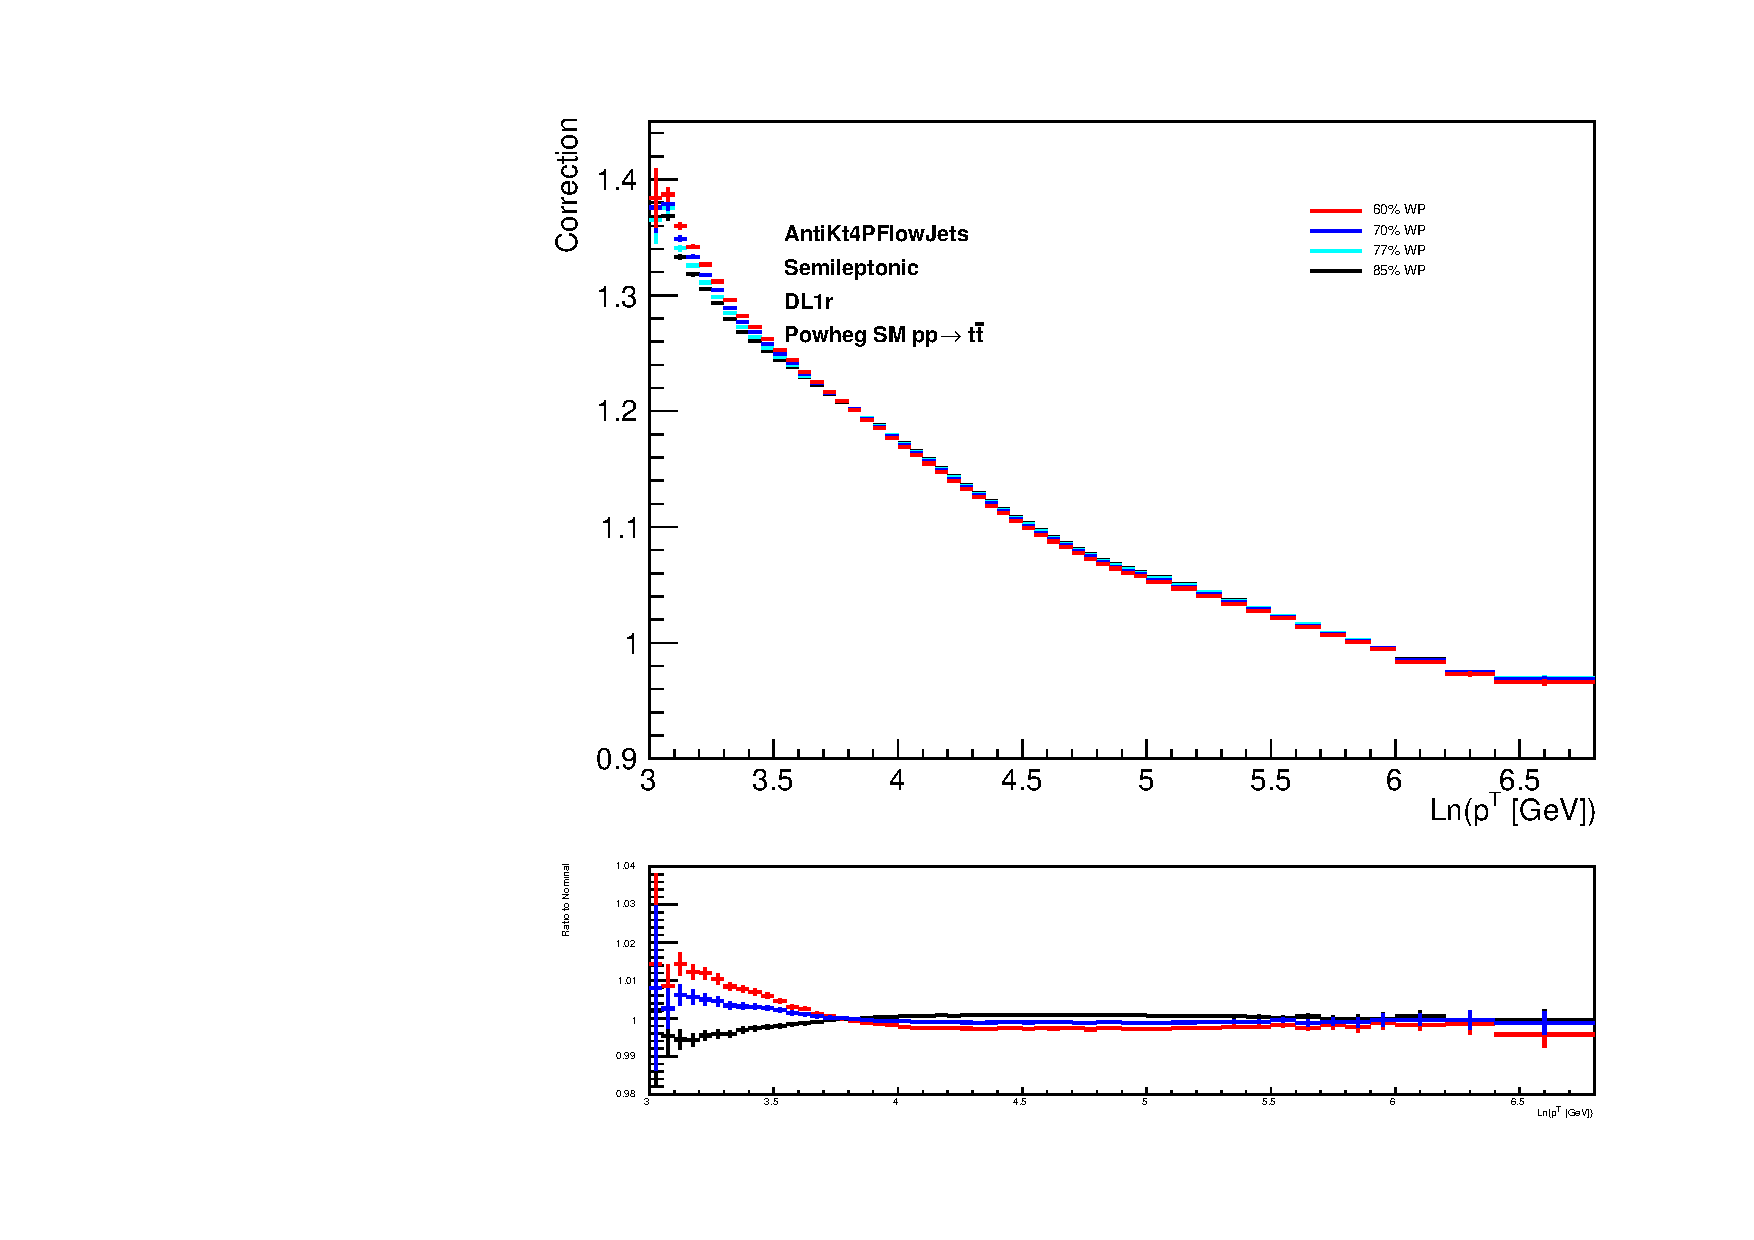
\includegraphics[width=.48\textwidth]{Ch5/Img/Semileptonic.pdf}}\quad
   \subfloat[Hadronic][Hadronic]{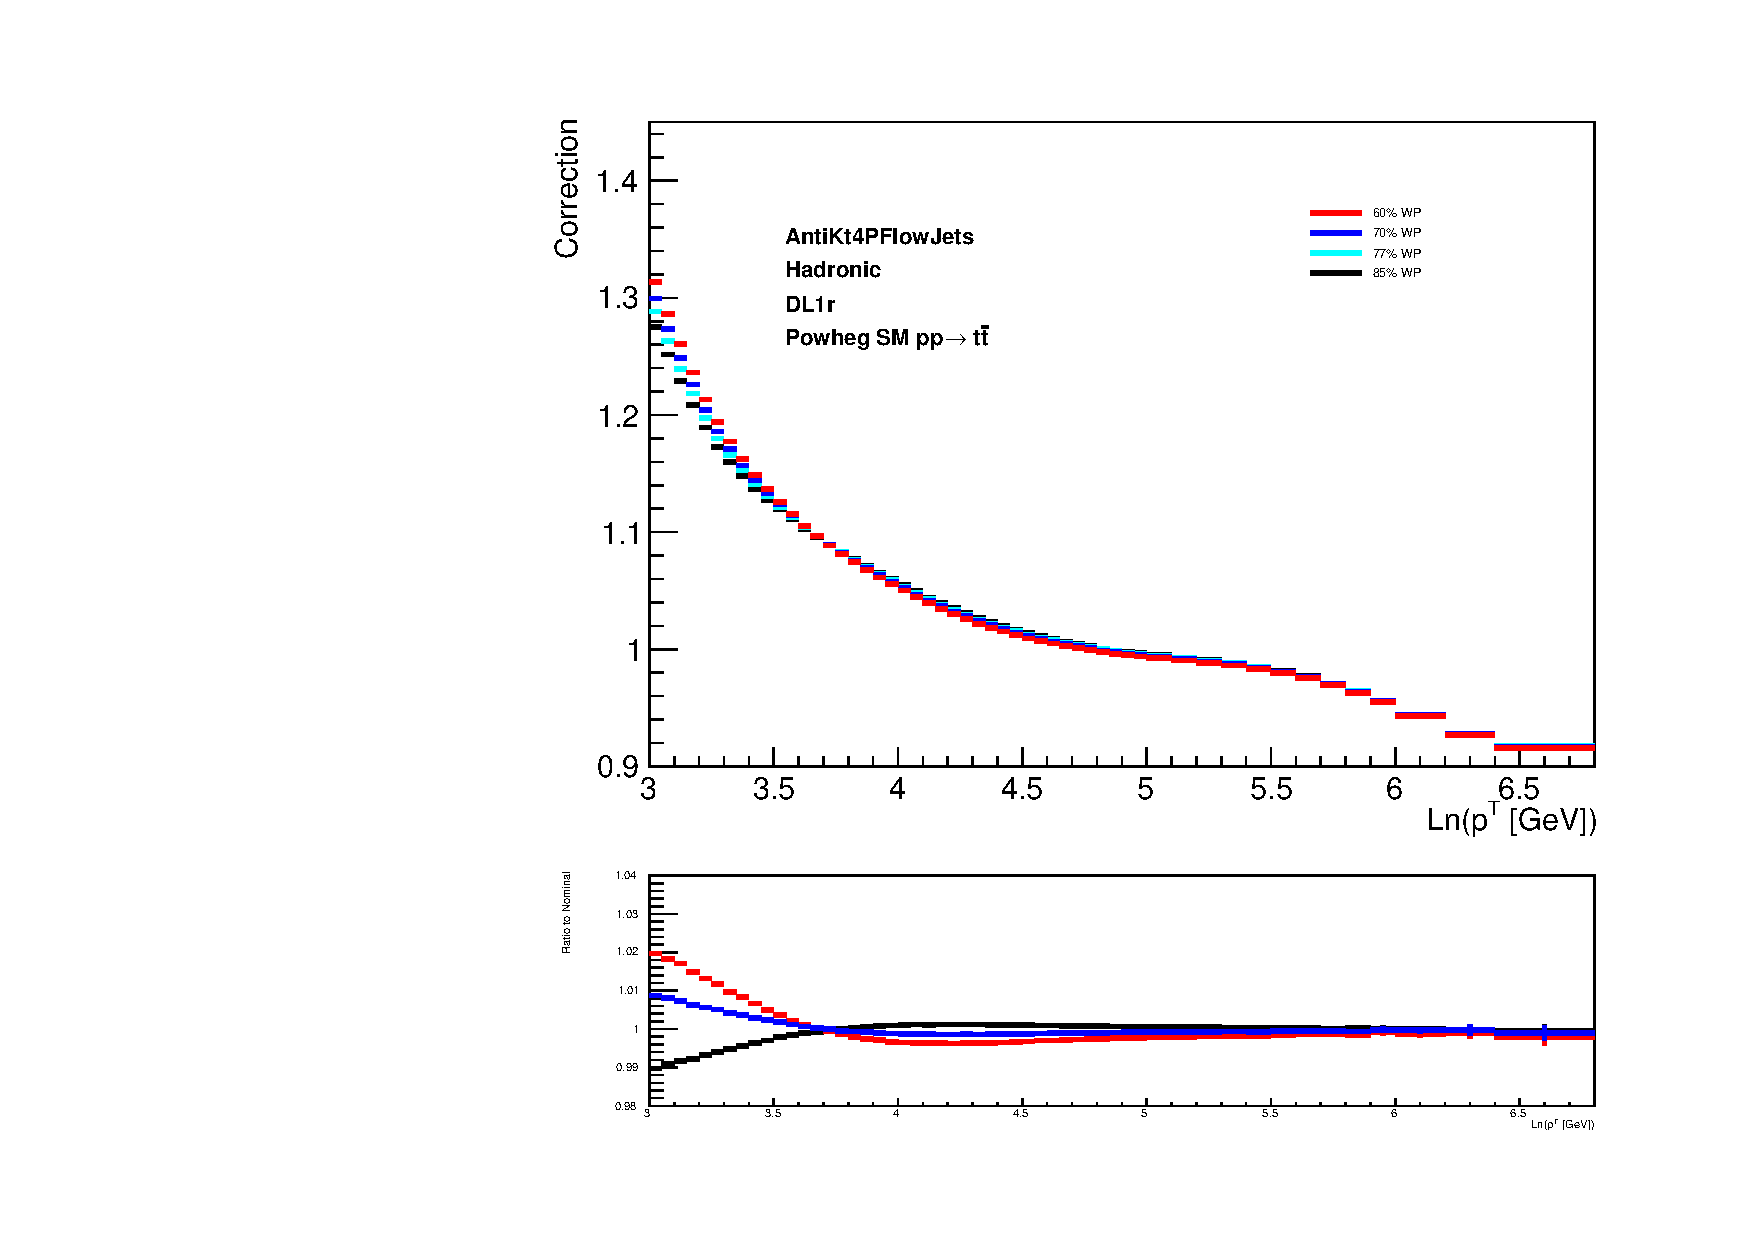
\includegraphics[width=.48\textwidth]{Ch5/Img/Hadronic.pdf}}
   \begin{tcolorbox}[colback=black!5!white,colframe=white!75!black]
   \caption{\pT-Reco correction distribution using different DL1r \bq-tagging WPs for both semileptonic (a) and hadronic (b) jets. Bottom panel shows the ratio of the \pT-Reco to the nominal (77\% WP). }
   \label{fig:HHyybb:Sys:Exp:PtReco}
   \end{tcolorbox}
   
\end{figure}
\\
The relative impact on the yield for a given correction function is used as a systematic uncertainty. \\
Table \ref{table_pt_reco_sys} summaries the relative effect of the nominal \pT-Reco correction on the yield. The impact on the shape is negligible for both the position and the spread. 
\begin{table}[ht!]
    \centering
    \begin{tabular}{lc}
        \hline
        \hline
        \pT-Reco variation & \% relative effect to nominal \\
        \hline
        60\% WP & $\pm$ 0.094 \\
        70\% WP & $\pm$ 0.065 \\
        85\% WP & $\pm$ 0.12 \\
        \hline
        \hline
    \end{tabular}
    \begin{tcolorbox}[colback=black!5!white,colframe=white!75!black]
    \caption{Relative \pT-Reco systematic uncertainty on the yield for given variation.}
    \label{table_pt_reco_sys}
    \end{tcolorbox}
\end{table}
\\
Even for 85\% WP (with a large acceptance)  which is related to the high amplitude of systematic uncertainties, it is of the same order as the flavour tagging uncertainty and therefore negligible compared to the jet energy scale and resolution uncertainties. Thus this systematic is neglected. 

\subsubsection{Theoretical systematic uncertainties}
\label{HHyybb:Syst:Theo}
Sources of systematic uncertainties related to the theory are considered:

\begin{itemize}
    \item QCD scale uncertainties: these are defined to account for the potential effect of missing higher order in the matrix element. These are estimated by varying the re-normalisation $\mu_R$ and the factorization $\mu_F$ scales coherently by a factor of 2 or 0.5 from their nominal values and recalculating the cross-section in each case. The largest deviation from the nominal cross-section across the \kl range [-10, 10] is taken as the uncertainty.  
    \item PDF+$\alpha_s$: account for the impact on the cross-sections of the choice of the PDF set as well as the $\alpha_{s}$ variation from its central value. These are taken from Ref. \cite{CERN_yellow} to be 3\% and kept constant over the full \kl range.
    \item Higgs boson branching ratio: accounts for the $H\to\gamma\gamma$ and $H\to b\bar{b}$ branching fractions uncertainties of the order of 2.9\% and 1.7\% respectively, taken also from Ref. \cite{CERN_yellow}. 
    \item Higgs boson mass: accounts for the Higgs boson mass measurement uncertainty of the order of 0.2\%, taken from Ref. \cite{Mass}. 
    \item Heavy flavour (HF): accounts for the uncertainty on the amount of select single ggF H, VBF H and WH events in which the two $b$-jets are probing a special phase space. This is considered to be 100\%.
    \item non-closure of \kl reweighting: account for the discrepancy in the \kl reweighting method as described in Section \ref{HHyybb:Data&MC}. 
\end{itemize}

\section{Statistical model}
\label{HHyybb:Stat}

The observed data is interpreted using the Modified Frequentist method ($CL_s$) \cite{CL_s}. A hypothesis test is made to evaluate the compatibility between the observed data and the background-only hypothesis for limit computation, which assumes no signal in the data. The test statistic used here is the profile likelihood ratio \cite{Z} built from signal+background model. The signal is extracted by performing a simultaneous maximum likelihood fit of the \myy distribution in the range [105, 160] GeV over the four categories. The likelihood is defined as: 
\begin{equation}
    \mathcal{L}=\prod_{c}\left(Pois\left(n_{c}
    \mid N_{c}(\theta)\right) \cdot \prod_{i=1}^{n_{c}}
    f_{c}\left(m_{\gamma \gamma}^{i}, \theta\right) \cdot G(\theta)\right),
\end{equation}
where for each event $i$ in a category $c$, $n_c$ is the observed number of events in real data, while $N_c$ is the expected number of event from simulation, 
$f_c$ the value of the pdf function, $\theta$ the nuisance parameters (systematic uncertainties) with G is their constraint pdfs. 
The expected number of events combines the signal HH from both ggF and VBF production modes, single Higgs boson backgrounds, the spurious signal and the continuum background, defined as: 
\begin{equation}
    N_{c}(\theta)=\mu \cdot N_{\mathrm{HH},
    \mathrm{c}}\left(\theta_{yield }\right)+N_{\mathrm{H},
    \mathrm{c}}\left(\theta_{yield }\right)+N_{\mathrm{SS},
    \mathrm{c}} \cdot \theta_{\mathrm{SS},
    \mathrm{c}}+N_{\text{continuum} , \mathrm{c}},
\end{equation}
where $\theta_{yield}$ and $\theta_{SS}$ are the systematics on the yield from experimental, theoretical uncertainties and spurious signal uncertainties. $\mu$ is the parameter of interest (POI) of the fit, (the signal strength) which measures the HH cross-section normalized to its SM predicted value. \\
The pdf $f_c$ is the sum of the DSCBs modelling the HH, single Higgs boson backgrounds and the spurious signal and the exponential function modelling the continuum background described in Section \ref{HHyybb:Modelling}. Only the signal strength, the exponential function parameter a, its normalization $N_{\text{continuum}}$ and the systematics uncertainties are allowed to float in the fit. \\
The profile likelihood ratio test is defined as: 
\begin{equation}
    \tilde{q}_{\mu}=\left\{\begin{array}{ll}
-2 \log \frac{L(\mu, \hat{\hat{\theta}}({\mu}))}{L(0, \hat{\hat{\theta}}(0))} & \hat{\mu}<0 \\
-2 \log \frac{L(\mu, \hat{\hat{\theta}}({\mu}))}{L(\hat{\mu}, \hat{\theta})} & 0 \leq \hat{\mu} \leq \mu \\
0 & \hat{\mu}>\mu
\end{array}\right.
\end{equation}
where $\hat{\mu}$ is the fit favoured signal strength, $\hat{\hat{\theta}}$ is the fit favoured nuisance parameter values when $\mu$ is fixed in the fit and $\hat{\theta}$ is the fit favoured nuisance parameter when $\mu$ is also floating. \\
In the absence of signal, an exclusion limit at 95\% Confidence Level (CL) is set on the \HHyybb cross-section for each \kl value in the range [-10, 10] with step of 0.2. The asymptotic approximation \cite{Z} is adopted here. A pseudo-data is used for the computation of the expected limits, called Asimov dataset. An Asimov dataset provides an idealized description of the predicted data with a given integrated luminosity without statistical fluctuations.

\section{Results}
\label{HHyybb:Results}

\subsection{Observed events and \myy fit}
\label{HHyybb:Results:Fit}
The results of the background-only fit of the \myy distribution for each category are shown in Figure \ref{fig:HHyybb:Results:Fit:myy}. 
\begin{figure}[htbp]
    \centering
    \subfloat[][High mass, BDT tight]{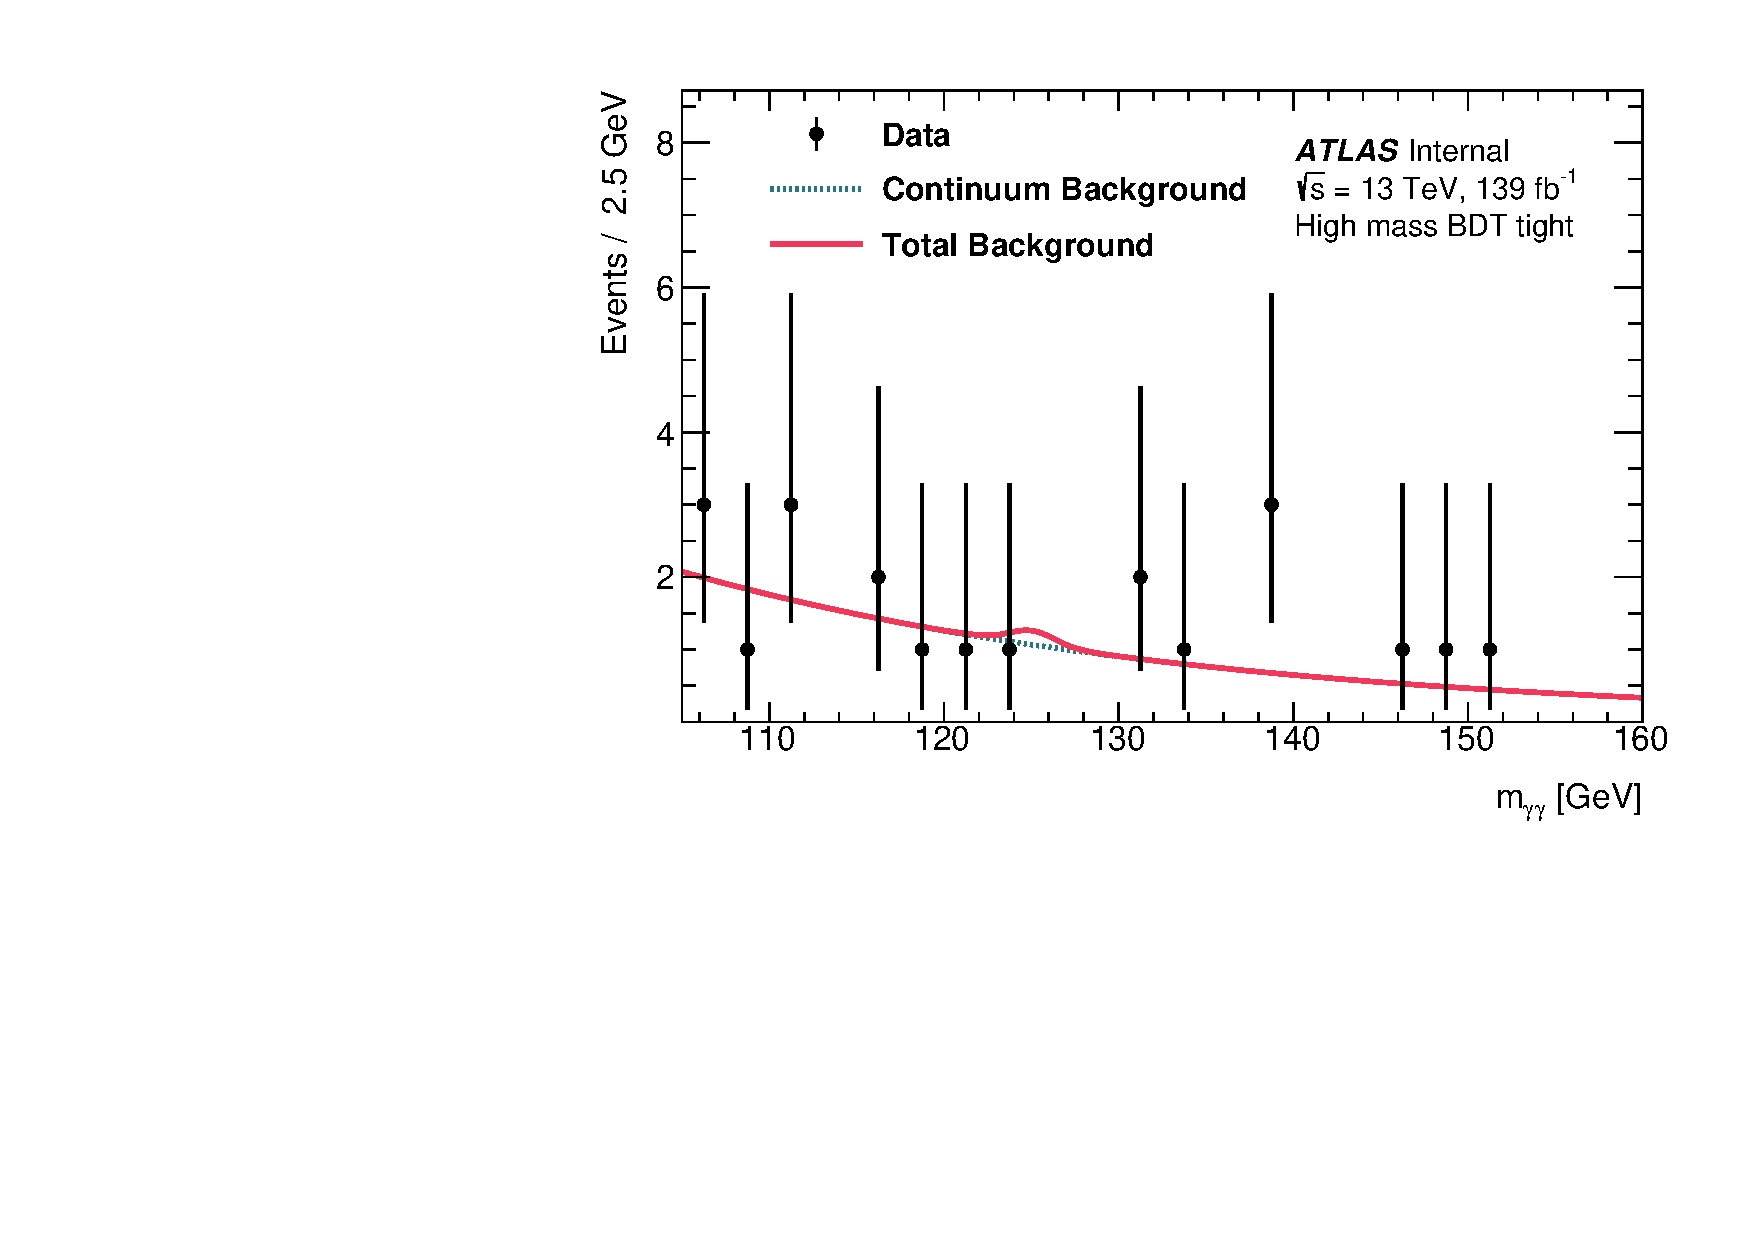
\includegraphics[width=.5\textwidth]{Ch5/Img/figures_Results_unweighted_yybb_SM_1_v2.pdf}}
    \subfloat[][High mass, BDT loose]{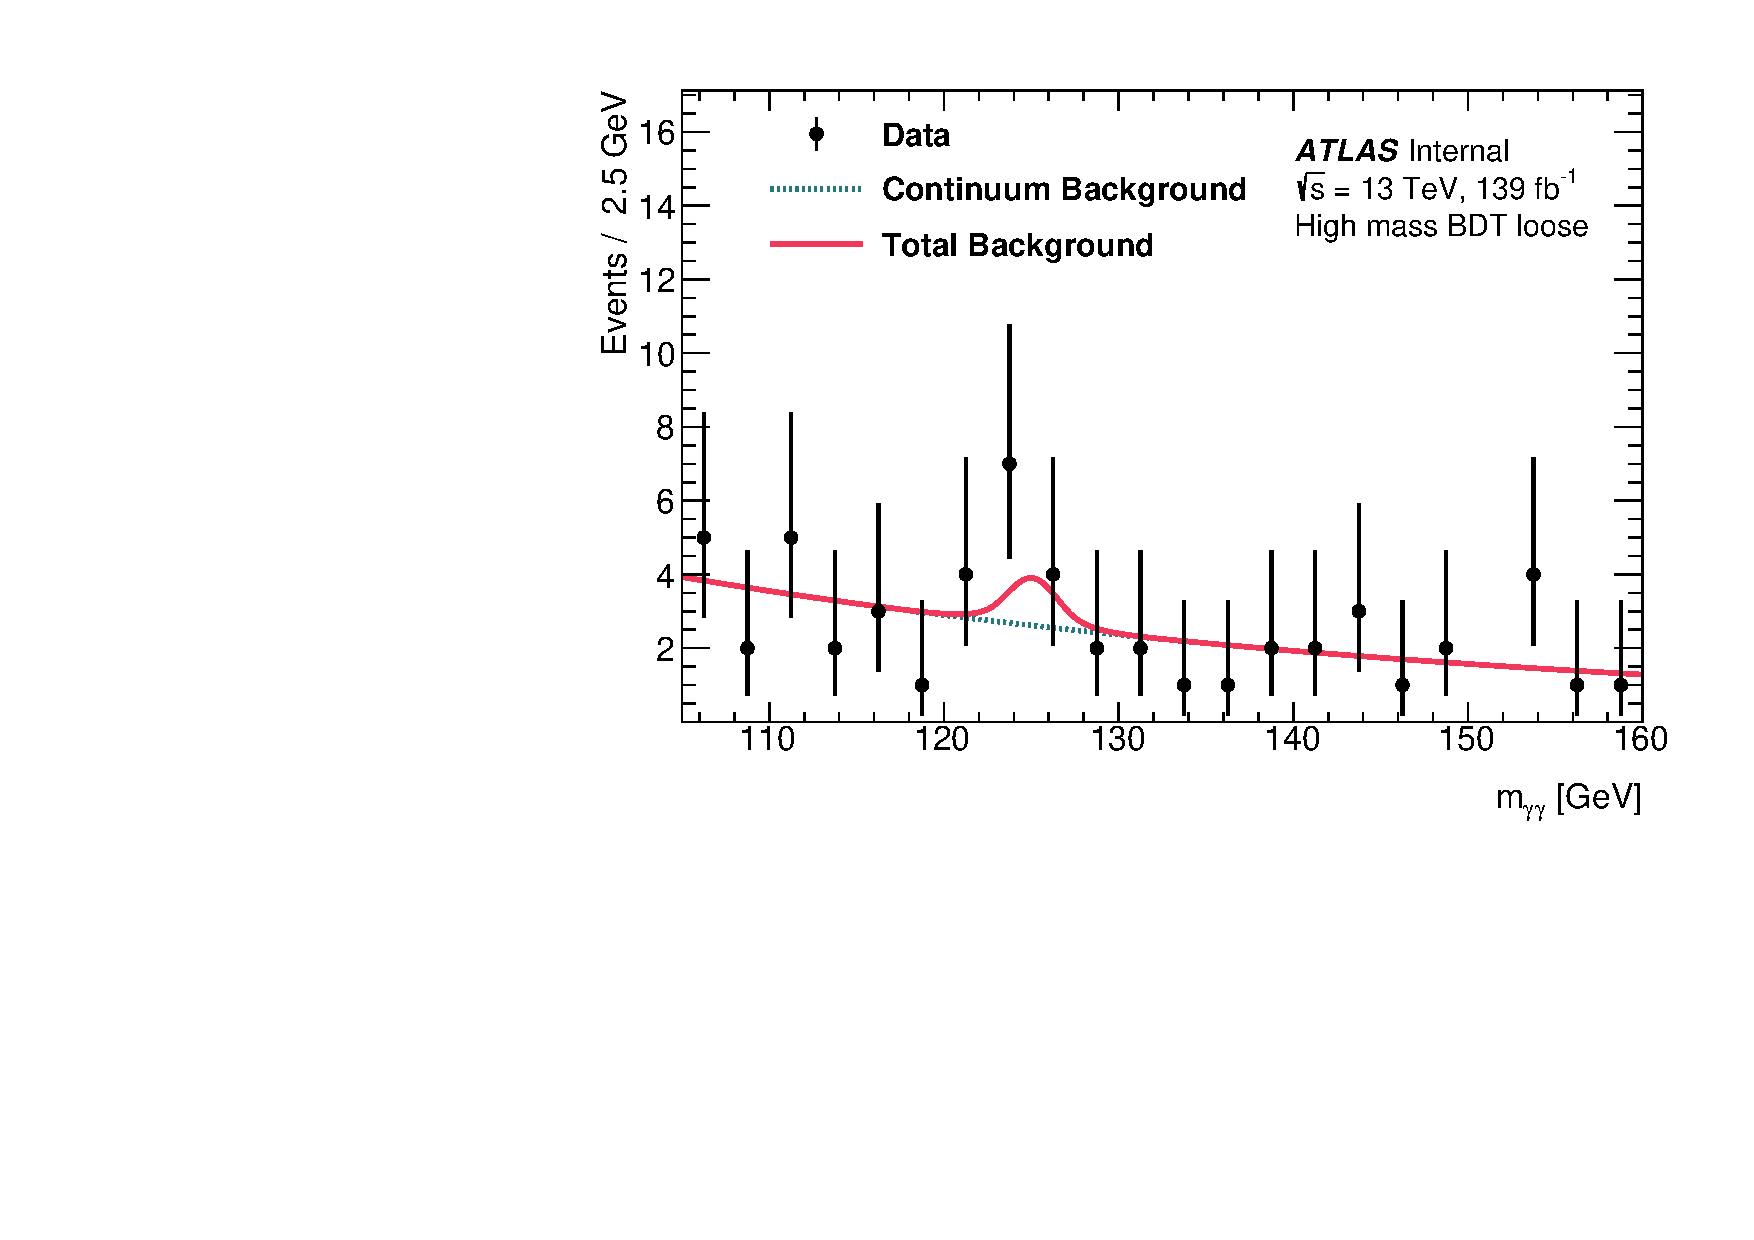
\includegraphics[width=.5\textwidth]{Ch5/Img/figures_Results_unweighted_yybb_SM_2_v2.pdf}} \\
    \subfloat[][Low mass, BDT tight]{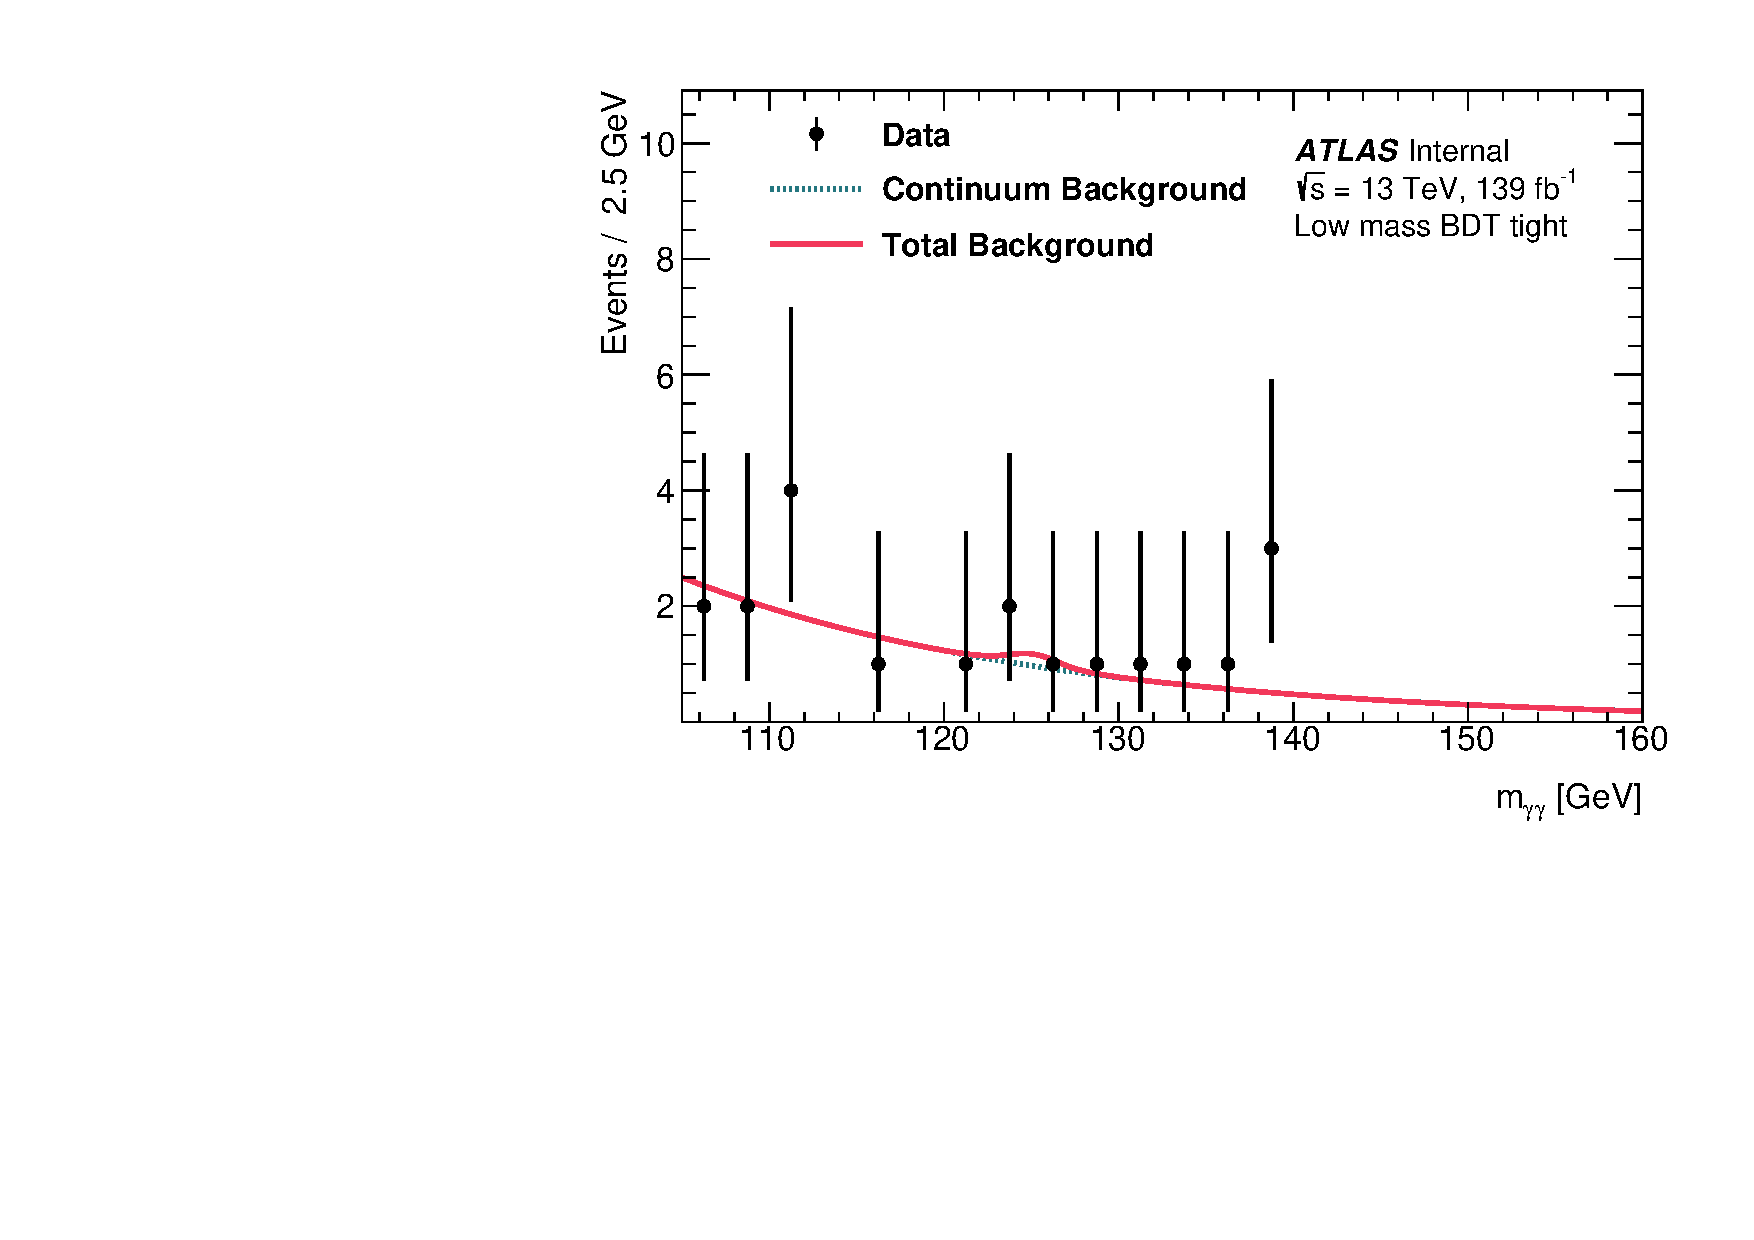
\includegraphics[width=.5\textwidth]{Ch5/Img/figures_Results_unweighted_yybb_BSM_1_v2.pdf}}
    \subfloat[][Low mass, BDT loose]{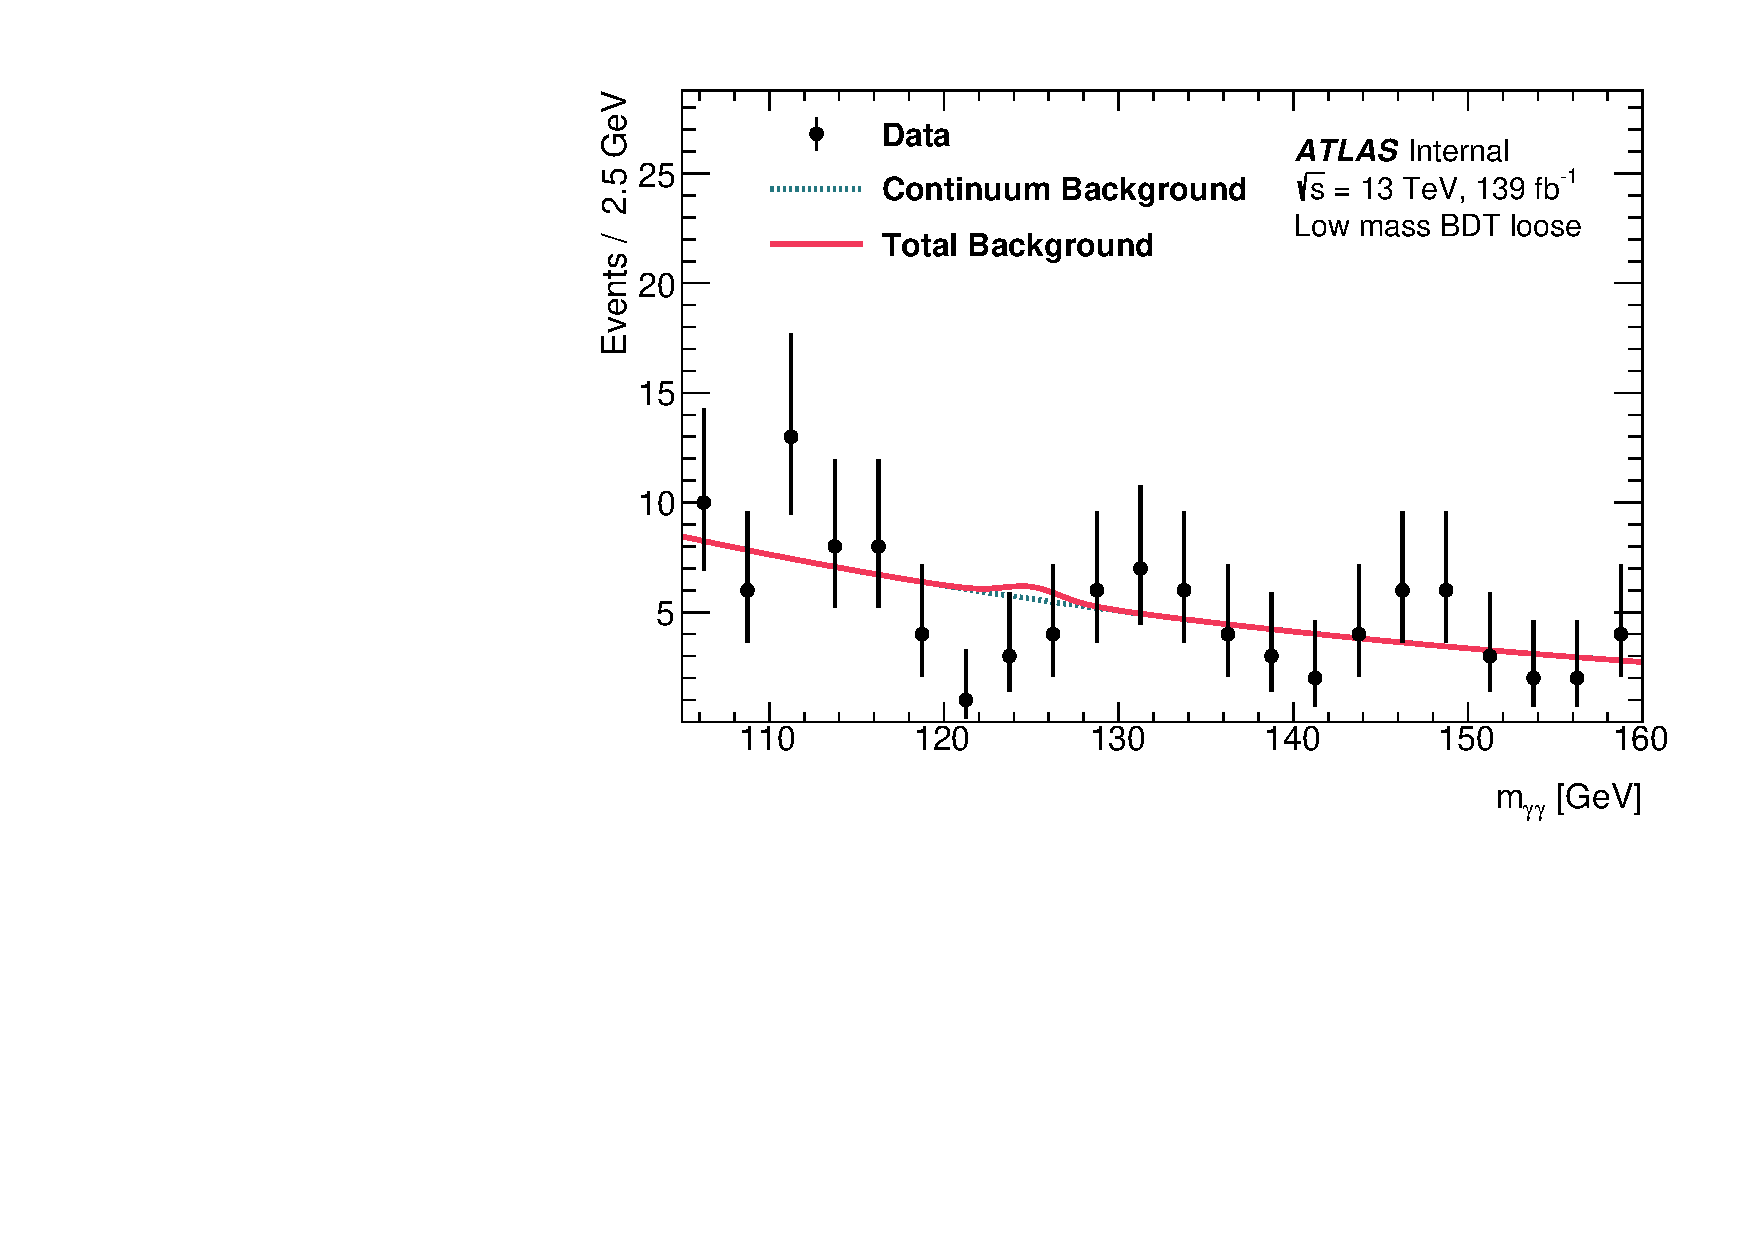
\includegraphics[width=.5\textwidth]{Ch5/Img/figures_Results_unweighted_yybb_BSM_2_v2.pdf}}
    \caption{The data points are compared to the background-only fit for the four BDT categories. Both the continuum background and the background from single Higgs boson production are considered.}
    \label{fig:HHyybb:Results:Fit:myy}
\end{figure}
The number of the observed and expected events in each category is summarized in Table  \ref{fig:HHyybb:Results:Fit:NEvt}.
\begin{table}[]
\centering
\begin{tabular}{ccccc}
\hline \hline
& High mass & High mass & Low mass & Low mass \\
& BDT tight & BDT loose & BDT tight & BDT loose \\
\hline
Continuum & $4.9 \pm 1.1$ & $9.5 \pm 1.5$ & $3.7 \pm 1.0$ & $24.9 \pm 2.5$ \\
\hline
Single Higgs boson & $0.670 \pm 0.032$ & $1.57 \pm 0.04$ & $0.220 \pm 0.016$ & $1.39 \pm 0.04$ \\
$\mathrm{ggF}$ & $0.261 \pm 0.028$ & $0.44 \pm 0.04$ & $0.063 \pm 0.014$ & $0.274 \pm 0.030$ \\
$t \bar{t} H$ & $0.1929 \pm 0.0045$ & $0.491 \pm 0.007$ & $0.1074 \pm 0.0033$ & $0.742 \pm 0.009$ \\
$Z H$ & $0.142 \pm 0.005$ & $0.486 \pm 0.010$ & $0.04019 \pm 0.0027$ & $0.269 \pm 0.007$ \\
Rest & $0.074 \pm 0.012$ & $0.155 \pm 0.020$ & $0.008 \pm 0.006$ & $0.109 \pm 0.016$ \\
\hline SM HH (\kl = 1) & $0.8753 \pm 0.0032$ & $0.3680 \pm 0.0020$ & $(49.4 \pm 0.7) \cdot 10^{-3}$ & $(78.7 \pm 0.9) \cdot 10^{-3}$ \\
$\quad \mathrm{ggF}$ & $0.8626 \pm 0.0032$ & $0.3518 \pm 0.0020$ & $(46.1 \pm 0.7) \cdot 10^{-3}$ & $(71.8 \pm 0.9) \cdot 10^{-3}$ \\
VBF & $0.01266 \pm 0.00016$ & $0.01618 \pm 0.00018$ & $(3.22 \pm 0.08) \cdot 10^{-3}$ & $(6.923 \pm 0.011) \cdot 10^{-3}$ \\
\hline BSM HH (\kl = 10) & $6.36 \pm 0.05$ & $3.691 \pm 0.038$ & $4.65 \pm 0.04$ & $8.64 \pm 0.06$ \\
\hline Data & 2 & 17 & 5 & 14 \\
\hline \hline
\end{tabular}
\caption{Expected and observed numbers of events in the signal region ([120, 130] GeV) for the four BDT categories. The uncertainties on the continuum background are those arising from the fitting procedure. The uncertainties on the single Higgs boson and Higgs boson pair production are from MC statistical error.}
\label{fig:HHyybb:Results:Fit:NEvt}
\end{table}

\subsection{Cross-section limits and \kl constraint}
\label{HHyybb:Results:Xsec}
 Since no significant excess over the background prediction is found, exclusion limits at 95\% CL are computed on the Higgs boson pair production cross-section for each \kl as described in Section $\ref{HHyybb:Stat}$. The upper limit obtained for the double Higgs boson production cross-section $\sigma_{HH}$ in the ggF + VBF production modes is 140 fb assuming \kl = 1. A median value of 180 fb is estimated. Expressed in terms of multiple of the SM production cross-section, the observed limit is 4.1 times the SM prediction while the expected limit is 5.5 times the SM prediction. The expected measured signal strength $\mu$ is 1 $\pm$ 2.37.\\

Constraint on the Higgs boson self-coupling is derived from the cross-section limit scan versus \kl by taking the intersection between the theoretical prediction and the measured cross-section, as shown in Figure \ref{fig:HHyybb:Results:Xsec:Limit}. The observed constraint at 95\% CL is -1.5 $<$ \kl $<$ 6.7, while the expected constraint is -2.4 $<$ \kl $<$ 7.7. BSM effects on the single Higgs boson cross-section and Higgs boson branching ratios are neglected. The couplings of Higgs boson to other particles are set to their SM values \cite{Higgs_80ifb}. Table \ref{tab:HHyybb:139ifb} summarizes the results. \\
In addition to the constraint, a measurement of \kl is performed by floating \kl in the fit with all other couplings set to their SM values. The best-fit \kl is $2.7^{+2.1}_{-2.2}$ which is close  to the \kl value giving the minimum HH cross-section. The likelihood scan as a function of \kl is shown in Figure \ref{fig:HHyybb:Results:Xsec:LH}.

\begin{table}[htbp]
    \centering
    \begin{tabular}{lcc}
    \hline \hline
         & Expected & Observed \\
         \hline 
    $\sigma_{HH}/\sigma_{HH}^{SM}$ limit & 5.5 & 4.1 \\
    \kl interval & [-2.4, 7.7] & [-1.5, 6.7] \\
    \hline\hline
    \end{tabular}
    \caption{Summary of \HHyybb limits at 95\% CL from the 139 \ifb analysis.}
    \label{tab:HHyybb:139ifb}
\end{table}
\begin{figure}[htbp]
    \centering
    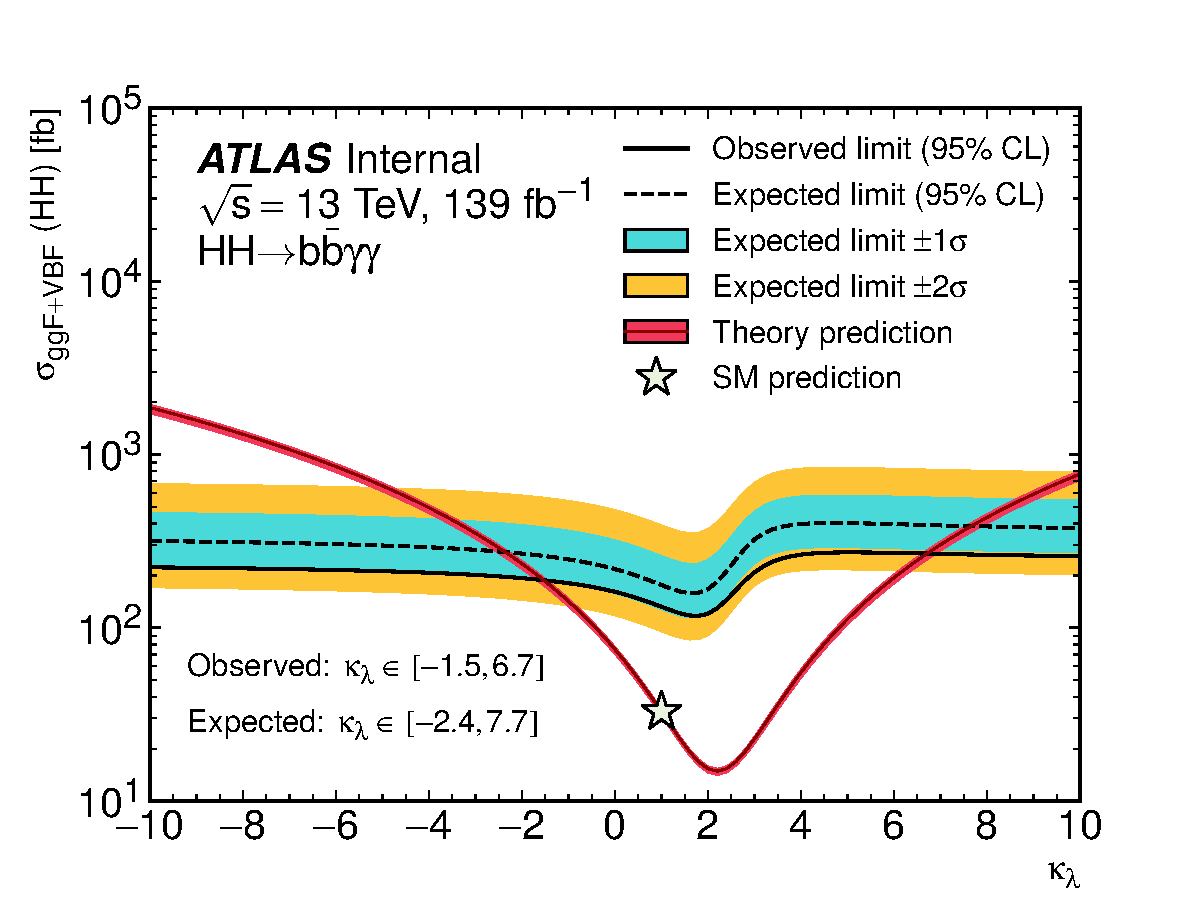
\includegraphics[width=0.5\textwidth]{Ch5/Img/figures_Results_kappa_lambda_scan.pdf}
    \caption{Observed and expected limits at 95\% CL on the cross-section of Higgs boson pair production as a function of the Higgs boson self-coupling modifier $\kappa_{\lambda}= \lambda_{HHH}/\lambda^{\textrm{SM}}_{HHH}$. The $\pm 1\sigma$ and $\pm 2\sigma$ bands show the expected variations on the expected limit due to statistical and systematic uncertainties. The theory prediction curve represents the scenario where all parameters and couplings are set to their SM values except for \kl. The uncertainty band of the theory prediction curve shows the cross-section uncertainty.}
    \label{fig:HHyybb:Results:Xsec:Limit}
\end{figure}

\begin{figure}[htbp]
    \centering
    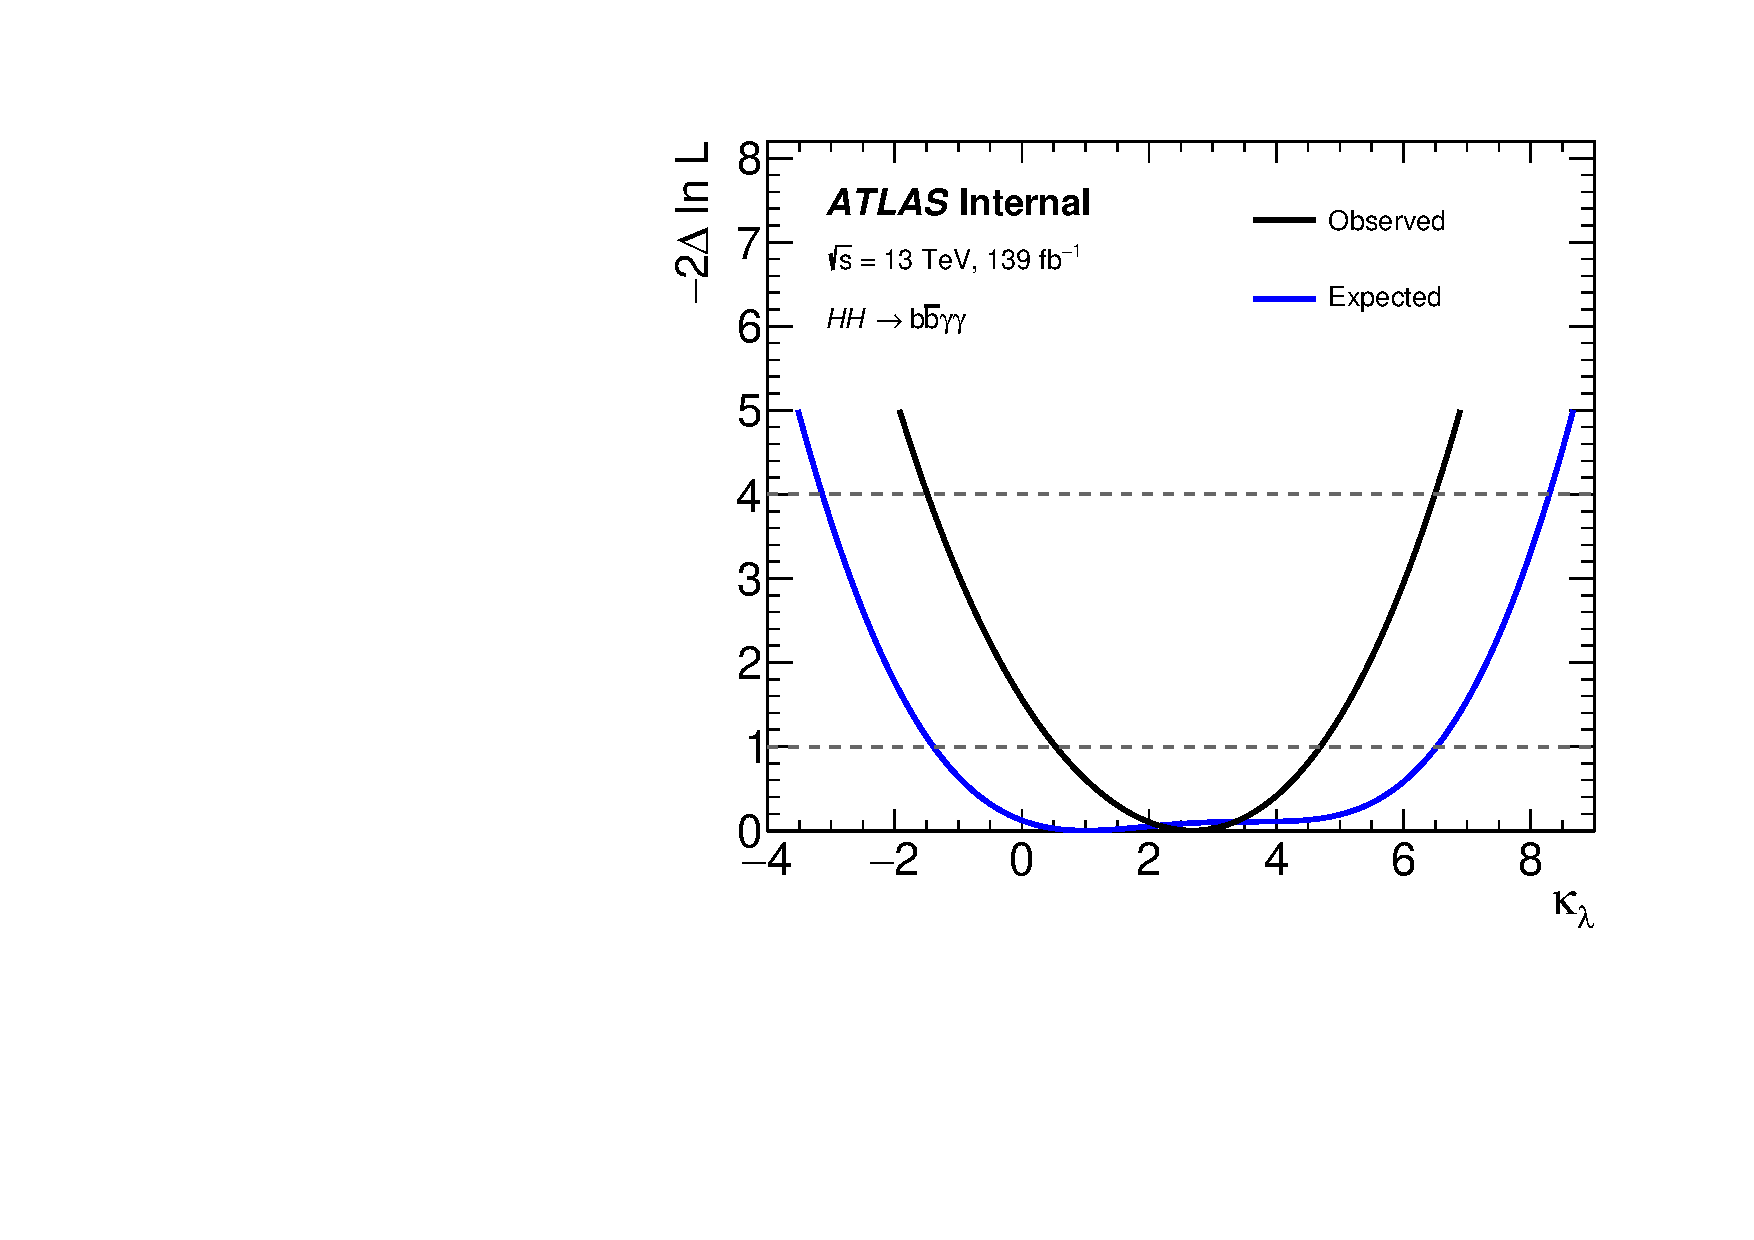
\includegraphics[width=0.5\textwidth]{Ch5/Img/figures_Results_scan_hhyybb_kl.pdf}
    \caption{The likelihood function as a function of \kl, with $\mu = $  1. The observed 68\% and 95\% CL ranges are [0.5, 4.7] and [-1.4, 6.5] respectively, while the expected are [-1.4, 6.4] and [-3.1, 8.2].}
    \label{fig:HHyybb:Results:Xsec:LH}
\end{figure}


Table \ref{tab:HHyybb:Results:Xsec:Cat} shows the expected limit at 95\% CL on the HH cross-section for each category. The significance is mainly driven by the High mass high BDT category. 

\begin{table}[htbp]
    \centering
    \begin{tabular}{lc}
        \hline\hline
        Category &  $\sigma_{HH}/\sigma_{HH}^{SM}$ limit \\
        \hline
        High mass, High BDT &  5.8 \\
        High mass, Low BDT &  21.0  \\
        Low mass, High BDT &  102.9 \\
        Low mass, Low BDT  &  125.6 \\
        \hline 
        Combined & 5.5 \\
        \hline\hline
    \end{tabular}
    \begin{tcolorbox}[colback=black!5!white,colframe=white!75!black]
    \caption{The expected limit on the HH cross-section at 95\% CL for each analysis category for SM case. The combined limit is also shown.}
    \label{tab:HHyybb:Results:Xsec:Cat}
    \end{tcolorbox}
\end{table}


Figure \ref{fig:HHyybb:Results:Xsec:statvsSys} shows the expected limit at 95\% CL on the cross-section of the HH pair production as a function of the \kl modifier for individual contributions of the statistical and statistical + systematic uncertainties. The statistical only limits are computed by setting all the systematic uncertainties to zero. Table \ref{tab:HHyybb:Results:Xsec:Stat} summarizes the upper limit for \kl = 1 case and the constraint on \kl for each systematic configuration. It shows that this search is statistically limited, and the total impact of systematic uncertainties on the results is about 4\%.
\begin{figure}[htbp]
    \centering
    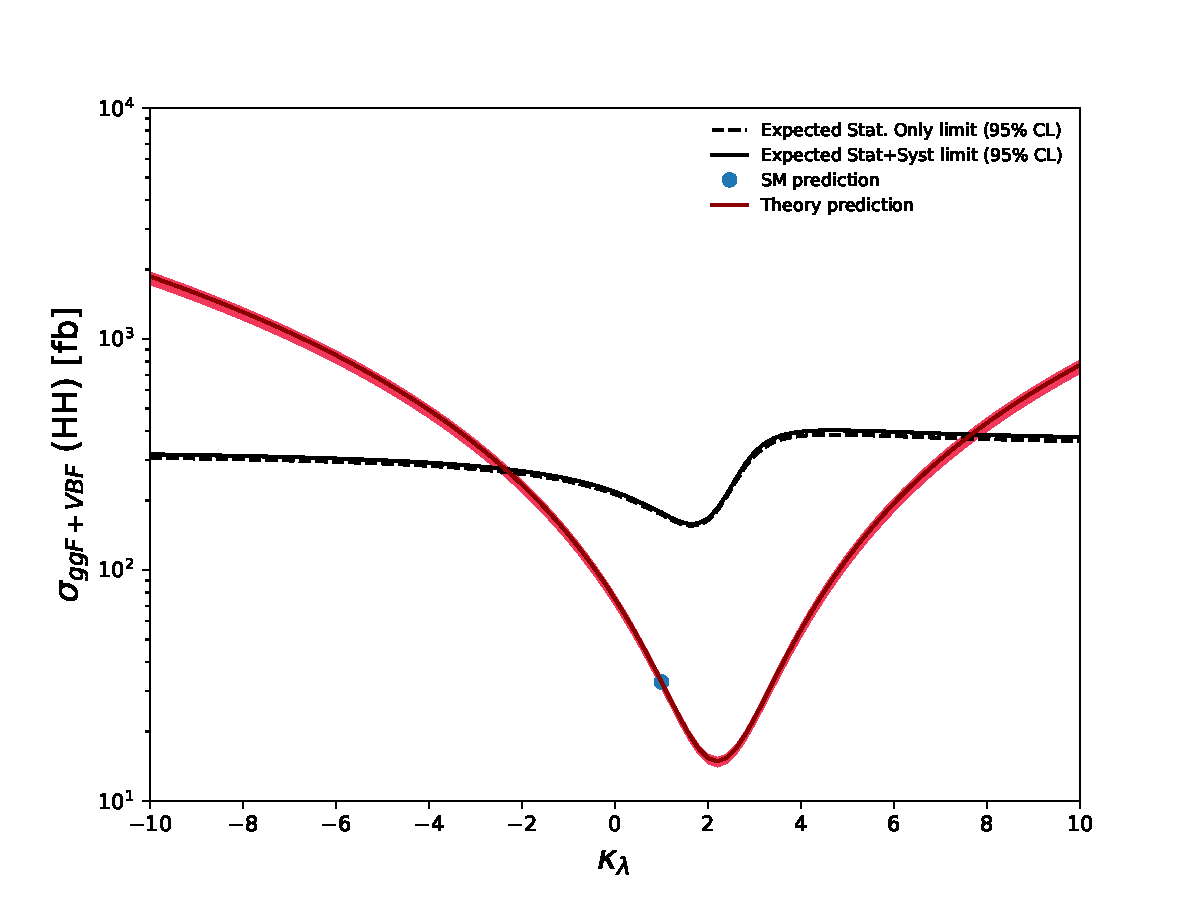
\includegraphics[width=0.5\textwidth]{Ch5/Img/kappa_lambda_stat_vs_sys.pdf}
    \begin{tcolorbox}[colback=black!5!white,colframe=white!75!black]
    \caption{Expected limits at 95\% CL on the cross-section of Higgs boson pair production as a function of the Higgs boson self-coupling modifier \kl for statistical only and statistical+systematic configurations. The luminosity is equal to 139 \ifb.}
    \label{fig:HHyybb:Results:Xsec:statvsSys}
    \end{tcolorbox}
\end{figure}
\begin{table}[htbp]
    \centering
    \begin{tabular}{lcc}
    \hline \hline 
         & Stat. Only & Stat.+Syst. \\
         \hline
        $\sigma_{HH}/\sigma_{HH}^{SM}$ limit & 5.3 & 5.5  \\
         \kl interval &  [-2.3, 7.6] &  [-2.4, 7.7]   \\
         \hline \hline
    \end{tabular}
    \begin{tcolorbox}[colback=black!5!white,colframe=white!75!black]
    \caption{Expected upper limit at 95\% CL on the cross-section of the HH pair production and allowed \kl interval for statistical only and statistical + systematic uncertainties}
    \label{tab:HHyybb:Results:Xsec:Stat}
    \end{tcolorbox}
\end{table}
\\
Table \ref{tab:HHyybb:Results:Xsec:Sys} shows the impact of the systematic uncertainties on the upper limit on the signal strength $\mu$. The dominant systematics are related to the spurious signal and the photon energy scale (PES) uncertainties. As mentioned in Section \ref{HHyybb:Syst:Exp}, the PES systematic arises from the measurement of photon energy and its calibration which is mainly induced by the cell non-linearity and the under-estimation of passive material in front of the calorimeter in simulation. The bias due to the background function choice leads to the large spurious signal uncertainties and mainly dominated by the statistical fluctuations of the continuum background statistics used in the spurious signal test. \\
Since simulating more events was however not possible in the timescale of the analysis, several attempts are done to improve the continuum statistics and reduce statistical fluctuation: 
\begin{itemize}
    \item The Gaussian Process Regression (GPR) \cite{GPR} is used to smooth and reduce fluctuations in the \myy distribution, this method reduces the $N_{SS}$ by 84\%.
    \item Increasing statistics by inverting the $b$-tagging requirements reduces the systematic on $\mu$ by $\sim$ 3\%.
\end{itemize}
Since the analysis is statistically dominated, the significance does not improve significantly, thus these improvements are not included in these results.  
\begin{table}[htbp]
    \centering
    \begin{tabular}{lcc}
\hline \hline 
Source & Type & Relative impact in \%  \\
\hline Experimental & & \\
\hline Photon energy scale & Norm. + Shape & 5.2  \\
Photon energy resolution & Norm. + Shape & 1.8  \\
Flavour tagging & Normalization & 0.5  \\
\hline Theoretical & & \\
\hline Heavy flavour content & Normalization & 1.5  \\
Higgs boson mass & Norm. + Shape & 1.8  \\
PDF+ $\alpha_{\mathrm{s}}$ & Normalization & 0.7  \\
\hline Spurious signal & Normalization & 5.5 \\
\hline \hline
\end{tabular}
    \caption{Breakdown of the dominant systematic uncertainties. Only systematic uncertainties with an impact of at least 0.5\% are shown. Uncertainties of Norm. + Shape type have effects on both the yield and the shape of the \myy distributions, the rest of uncertainties affect only the yields.}
    \label{tab:HHyybb:Results:Xsec:Sys}
\end{table}

\section{Comparison to 36 \ifb results}
\label{HHyybb:36ifb}
Table \ref{tab:HHyybb:36ifb} compares the observed and expected limits as well as the constraint on \kl derived with 36 \ifb and 139 \ifb datasets \cite{yybb_36ifb, yybb_139}. The limit in the 139 \ifb is improved compared to 36 \ifb analysis by a factor 5. The improvement is coming from both the increase by factor a 3.9 of the integrated luminosity and the new analysis strategy. By extrapolating the 36 \ifb results to 139 \ifb, the new analysis strategy improves the limit by a factor 2.4. Such improvement is mainly coming from the implementation of machine learning in event categorization (BDT) and the split in the two $m_{b\bar{b}\gamma\gamma}^*$ bins (High/Low mass).\\
In addition to the analysis strategy, the 139 \ifb analysis benefits from several improvements such as the usage of the PFlow algorithm for jet reconstruction which improves jet resolution as well as the specific $b$-jet energy calibration which enhances the analysis sensitivity by $\sim$ 10\%. The $b$-tagging efficiency is also improved by moving from the MV2c10 algorithm to the DL1r which has a higher efficiency as shown in Figure \ref{fig:Jet:Tag:Dlr:Eff_77}. \\
Considering the VBF production mode for the first time as a part of the signal when setting limits on \kl brings an improvement of 6-8\% in \kl interval. 

\begin{table}[htbp]
    \centering
    \begin{tabular}{lcccc}
    \hline \hline
         & Expected & Observed & Expected & Observed \\
         & 36 \ifb  & 36 \ifb  & 139 \ifb & 139 \ifb \\
         \hline 
    $\sigma_{HH}/\sigma_{HH}^{SM}$ limit & 28 & 22 & 5.5 & 4.1 \\
    \kl interval & [-8.3, 13.2] & [-8.2, 13.2] & [-2.4, 7.7] & [-1.5, 6.7] \\
    \hline\hline
    \end{tabular}
    \caption{Summary of \HHyybb results from 36 \ifb and 139 \ifb analyses.}
    \label{tab:HHyybb:36ifb}
\end{table}


\section{Comparison to CMS \HHyybb results}
\label{HHyybb:CMS}
The CMS collaboration published its results of the search of \HHyybb based on the data collected by the CMS detector between 2015 and 2018 which corresponds to 137 \ifb \cite{CMS_yybb}. Similarly to ATLAS, no significant deviation from the background-only hypothesis was found. The analysis strategy is very different from the ATLAS one presented in this thesis. It leads to different limits and \kl measurement. Due to the differences in the analysis strategies, a direct comparison is not trivial. The results obtained by CMS on the limit are presented in Figure \ref{fig:HHyybb:CMS:Xsec} and compared to ATLAS in Table \ref{tab:HHyybb:CMS}. The \kl likelihood scan is shown in Figure \ref{fig:HHyybb:CMS:kl:LH}. CMS results are extracted from a simultaneous fit of (\myy, \mbb) divided in fourteen analysis categories (on MVA output and $m_{b \bar{b} \gamma \gamma}^{*}$) defined using several MVA techniques and containing twelve ggF HH categories and two VBF HH dedicated categories. In contrary to ATLAS, CMS defines dedicated categories to target the VBF HH. In addition, CMS provides a specific orthogonal category to target $t\bar{t}$H to set constraints on the \kt modifier. Both HH and single Higgs boson are combined to provide an improved constraint of the \kl and \kt parameters. The inclusion of the $t\bar{t}$H significantly improves the constraint on \kt as demonstrated in the 2D likelihood scan of \kl and \kt in Figure \ref{fig:HHyybb:CMS:LH:2D}. Besides this, CMS uses two machine learning based techniques to improve the $b$-jet energy:
\begin{itemize}
    \item a DNN approach to improve the energy of resolution similarly to the method presented in Section \ref{Jet:Cal:BCal}.
    \item additional BDT approach which uses the fact that there is no missing transverse momentum from the hard-scattering process in the \HHyybb final state to correct the \mbb invariant mass which is similar to the kinematic fit described in Appendix \ref{Adx4}.
\end{itemize}
CMS uses a 2D fit of \myy and \mbb, while ATLAS only \myy as the final discriminant variable. The 2D fit was considered in the ATLAS analysis but not implemented, since similar improvements was obtained between the 2D fit and including the \mbb in the MVA training.
%while it brought some additional technical complexity , its implementation is kept more next round. 

\begin{figure}[htbp]
    \centering
    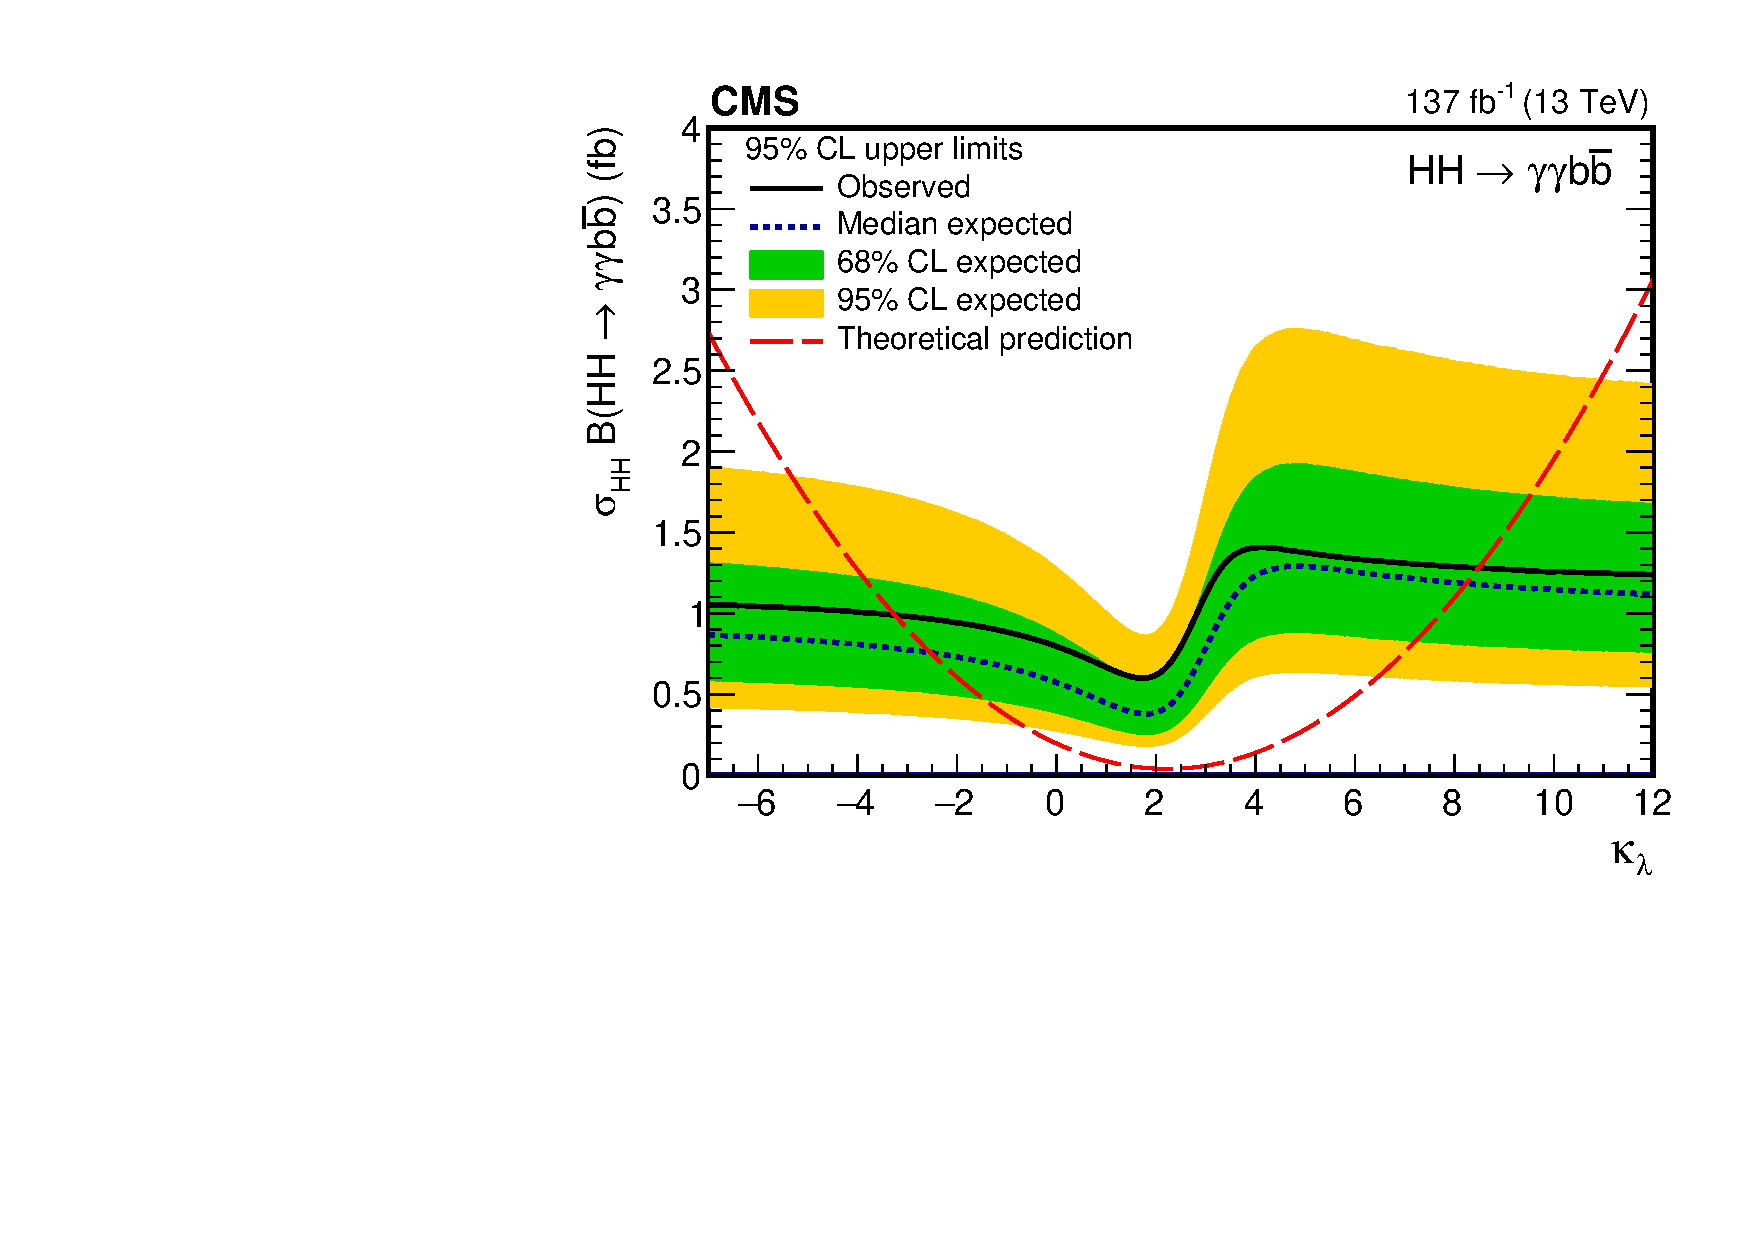
\includegraphics[width=0.5\textwidth]{Ch5/Img/CMS-HIG-19-018_kl_scan.pdf}
    \caption{Expected and observed 95\% CL upper limits on the \HHyybb cross-section obtained for different values of \kl assuming \kt = 1. The green and yellow bands represent, respectively, the one and two standard deviation. The long-dashed red line shows the theoretical prediction. }
    \label{fig:HHyybb:CMS:Xsec}
\end{figure}

\begin{table}[htbp]
    \centering
    \begin{tabular}{lcc}
    \hline \hline
         & Expected & Observed\\
         \hline 
   CMS  $\sigma_{HH}/\sigma_{HH}^{SM}$ limit & 5.2 & 7.7 \\
   CMS \kl interval & [-2.5, 8.2] & [-3.3, 8.5]  \\
    \hline
    ATLAS  $\sigma_{HH}/\sigma_{HH}^{SM}$ limit & 5.5 & 4.1 \\
    ATLAS \kl interval & [-2.4, 7.7] & [-1.5, 6.7] \\
    \hline \hline
    \end{tabular}
    \caption{Summary of ATLAS and CMS \HHyybb results. The limit is presented as a multiple of the SM expected value.}
    \label{tab:HHyybb:CMS}
\end{table}

\begin{figure}[htbp]
    \centering
    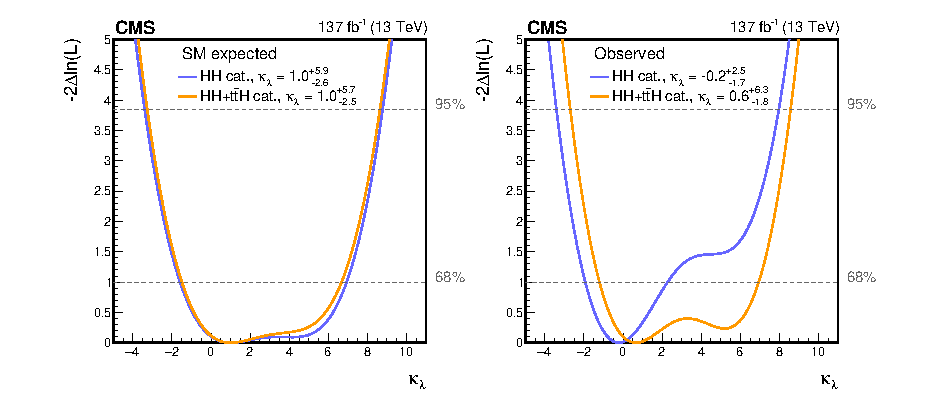
\includegraphics[width=0.85\textwidth]{Ch5/Img/CMS-HIG-19-018_kl_kt_LH.pdf}
    \caption{Negative log-likelihood, as a function of \kl, evaluated with an Asimov data set assuming the SM hypothesis. The 68 and 95\% CL intervals are obtained from the intersection with the dashed grey lines. The two curves are shown for the HH (blue) and HH+$t\bar{t}$H (orange) analysis categories. All other couplings are set to their SM values.}
    \label{fig:HHyybb:CMS:kl:LH}
\end{figure}

\begin{figure}[htbp]
    \centering
    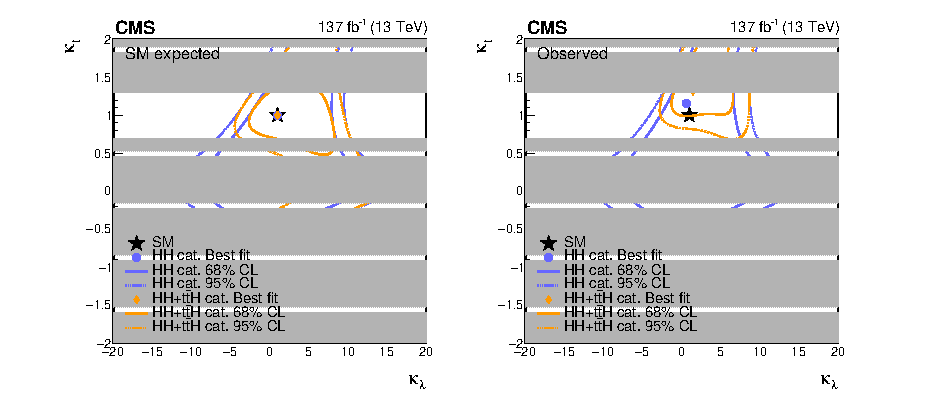
\includegraphics[width=0.85\textwidth]{Ch5/Img/CMS-HIG-19-018_kl_LH.pdf}
    \caption{Negative log-likelihood contours at 68 and 95\% CL in the (\kl, \kt) plane evaluated with an Asimov data set assuming the SM hypothesis (left) and the observed data (right). The contours obtained using the HH analysis categories only are shown in blue, and in orange when combined with the $t\bar{t}$H categories. The best fit value for the HH categories only (\kl = 0.6, \kt = 1.2) is indicated by a blue circle, for the HH + $t\bar{t}$H categories (\kl = 1.4, \kl = 1.3) by an orange diamond, and the SM prediction (\kl = 1.0, \kt = 1.0) by a black star. The grey band shows the region where LO parametrization of \kt used in CMS analysis is not reliable. }
    \label{fig:HHyybb:CMS:LH:2D}
\end{figure}


CMS shows a slightly better expected cross-section limit than ATLAS, which could be explained by the dedicated VBF category. ATLAS shows a more precise \kl constraint which is related to the under-optimization done by CMS when defining the analysis ggF HH regions. In the CMS analysis, categories on $m_{b \bar{b} \gamma \gamma}^{*}$ are defined after the MVA is trained, while in ATLAS the training is done separately in each $m_{b \bar{b} \gamma \gamma}^{*}$ category with specific signal as described in Section \ref{HHyybb:ObjEvt:Evt}. The signal used by CMS as training sample is a mixture of SM HH and 12 BSM benchmarks proposed in Ref. \cite{CMS_BSM}, but the mixing procedure is not explained in their published article. The training strategy used by ATLAS seems to improve the MVA performance in each $m_{b \bar{b} \gamma \gamma}^{*}$ region, giving better sensitivity to \kl which is mainly derived by the low mass category. As consequence, even with lower di-photon trigger threshold and better photon energy resolution, CMS measurement is slightly less precise. \\

Since ATLAS and CMS results could be considered similar, the ATLAS+CMS \HHyybb combination is equivalent to twice the ATLAS only. Given this assumption, the ATLAS+CMS combination is approximated by scaling the ATLAS \HHyybb luminosity with a factor 2. \\
The statistical-only expected limit on the HH cross-section for both ATLAS and ATLAS+CMS approximation is shown in Figure \ref{fig:HHyybb:CMS+ATLAS}. The expected 95\% CL upper limits on the HH cross-section for the SM case from the ATLAS+CMS approximation is 3.5 times the SM expectation and the expected allowed \kl interval is [-1.2, 6.6] at 95\% CL. 

\begin{figure}[htbp]
    \centering
    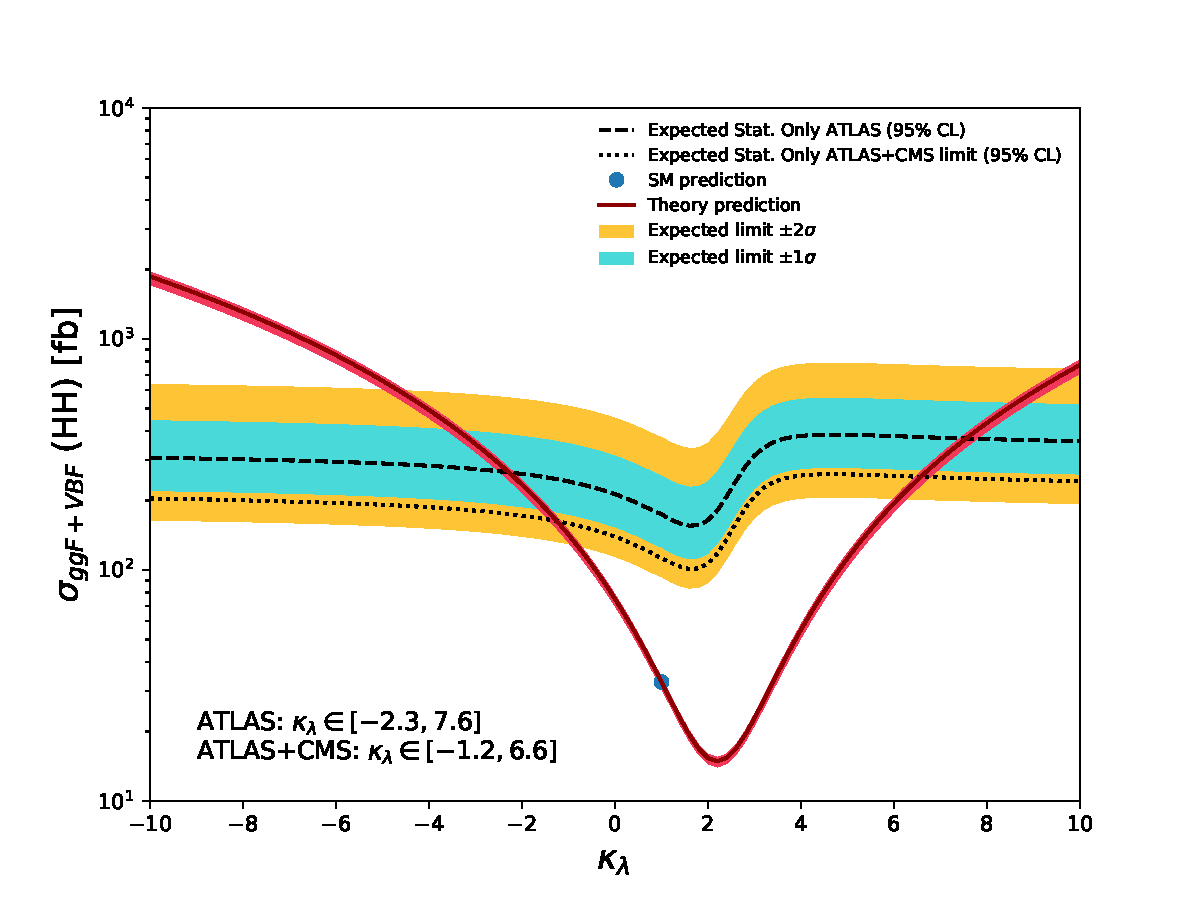
\includegraphics[width=0.6\textwidth]{Ch5/Img/kappa_lambda_ATLAS_CMS_stat.pdf}
    \begin{tcolorbox}[colback=black!5!white, colframe=white!75!black]
    \caption{The stat. only expected 95\% CL upper limits on the HH cross-section obtained for different values of \kl. Approximate ATLAS+CMS expected limits are obtained by scaling the ATLAS luminosity by a factor 2. The $\pm1\sigma$ and $\pm2\sigma$ bands are shown for the ATLAS expected limits.}
    \label{fig:HHyybb:CMS+ATLAS}
    \end{tcolorbox}
\end{figure}


\section{Comparison to other HH decay channels}
\label{HHyybb:HH}
As discussed in Section \ref{chap1:HH:HPD}, other production modes are sensitive to the Higgs boson self-coupling. In the following, the final states \bbbb, \bbtt channels are discussed. When this thesis is written, the full Run-2 analyses of these two channels are not yet published. As a consequence, only the 2015-2016 data results will be considered.

\subsection{\bbbb channel}
\label{HHyybb:HH:4b}
In the \bbbb analysis, the two Higgs boson of the HH system are reconstructed from 4 $b$-tagged jets with an invariant mass of each pair of $b$-tagged jets close to $m_{H}$. Only 27.5 \ifb of the data collected between 2015 and 2016 was used due to an inefficiency in the online vertex reconstruction affecting $b$-jet triggers. The invariant mass $m_{HH}$ of the two Higgs boson is used a discriminant variable. A large background remains after selection, mainly coming from QCD multi-jets (95\%) and $t\bar{t}$ events (5\%). A fully data-driven method is used to estimate the QCD multi-jets and $t\bar{t}$ backgrounds. Even with a large branching ratio ($\sim$ 33\%), the \bbbb channel suffers from very large backgrounds. Table \ref{tab:HHyybb:HH:4b} summarizes the limit on the HH cross-section and the constraint on the \kl. 
\begin{table}[htbp]
    \centering
    \begin{tabular}{lcc}
    \hline\hline
        & Expected & Observed \\
    \hline    
        $\sigma_{HH}/\sigma_{HH}^{SM}$ & 21 & 12.9 \\
        \kl interval & [-11.6, 18.8] & [-10.9, 20.1] \\
    \hline\hline
    \end{tabular}
    \caption{The 95\% confidence limits of the HH production cross-section in \bbbb channel and \kl interval.}
    \label{tab:HHyybb:HH:4b}
\end{table}

\subsection{\bbtt channel}
\label{HHyybb:HH:tt}

For the \bbtt analysis, HH events are reconstructed from two $b$-tagged jets and two $\tau$-leptons. The analysis consists in splitting events into two categories according to the $\tau^+\tau^-$ decay channels: 

\begin{itemize}
    \item the $\tau_{lep}\tau_{had}$ category, in which one of the two $\tau$s is decaying leptonically and the other hadronically. A single lepton trigger (SLT) is used.
    \item the $\tau_{had}\tau_{had}$ in which both $\tau$s are decaying hadronically. A SLT or di-tau triggers (DTT) are used.
\end{itemize}
The two categories are combined. A BDT is used to improve the separation between signal and background. Similarly to the \bbbb channel, the dominant background processes are the $t\bar{t}$, QCD multi-jets and Z bosons produced in association with jets originating from heavy-flavour quarks as well as the irreducible ZH background. Data-driven methods are used to estimate the background contamination. The \bbtt uses the BDT score as a discriminating variable to extract the results, which is less sensitive to \kl variations as shown in Figure \ref{fig:HHyybb:HH:tt}. Table \ref{tab:HHyybb:HH:tt} summarizes the limit on the HH cross-section and the constraint on the \kl parameter.

\begin{figure}[htbp]
    \centering
    \subfloat[][$\tau_{lep}\tau_{had}$]{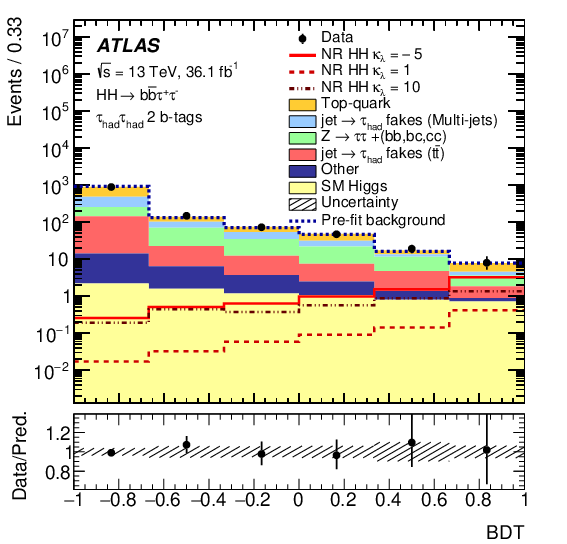
\includegraphics[width=.35\textwidth]{Ch5/Img/bbtt_BDT_lephad.png}}
    \subfloat[][$\tau_{had}\tau_{had}$]{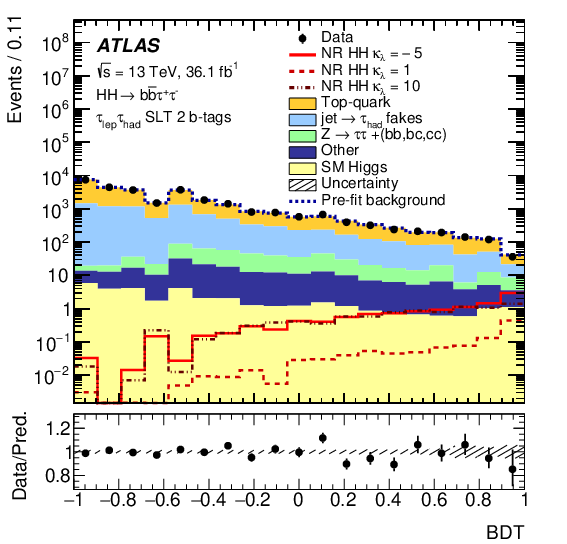
\includegraphics[width=.35\textwidth]{Ch5/Img/bbtt_BDT_hadhad.png}}
    \caption{The BDT distributions in the \bbtt analysis for the $\tau_{lep}\tau_{had}$ and $\tau_{had}\tau_{had}$ categories.}
    \label{fig:HHyybb:HH:tt}
\end{figure}

\begin{table}[htbp]
    \centering
    \begin{tabular}{lccc}
    \hline\hline
        & Expected & Observed \\
    \hline    
       $\tau_{lep}\tau_{had}$ $\sigma_{HH}/\sigma_{HH}^{SM}$ & 28.4 & 23.5 \\
       $\tau_{had}\tau_{had}$ $\sigma_{HH}/\sigma_{HH}^{SM}$ & 17.4 & 16.4 \\
       \hline 
      Combined $\sigma_{HH}/\sigma_{HH}^{SM}$ & 14.8 & 12.7 \\
      Combined \kl interval & [-8.9, 16.8] & [-7.4, 15.7] \\
    \hline\hline
    \end{tabular}
    \caption{The 95\% confidence limits on the HH production cross-section and \kl for the \bbtt analysis.}
    \label{tab:HHyybb:HH:tt}
\end{table}

%At time of writing, the full Run-2 \bbtt results are not published, while they are expected to be similar to the \bbyy full Run-2 analysis with an increase of 40\% in luminosity. Considering this, the stat. only combination of the full Run-2 \bbtt and \bbyy can be approximated with the \bbyy scaled to 2.4. The stat. only expected 95\% CL limits on the HH cross-section as a function of \kl with the approximated combination of \bbyy and \bbtt full Run-2 statistics is shown in Figure \ref{fig:HHyybb:HH:tt:Comb}. The expected stat. only upper 95\% CL limit on the Higgs pair production cross-section by combining \bbyy and \bbtt full Run-2 results is approximated to 3.1 times the SM expectation. The allowed \kl interval from the approximated combination is [-1., 6.4].

%\begin{figure}[htbp]
%    \centering
%    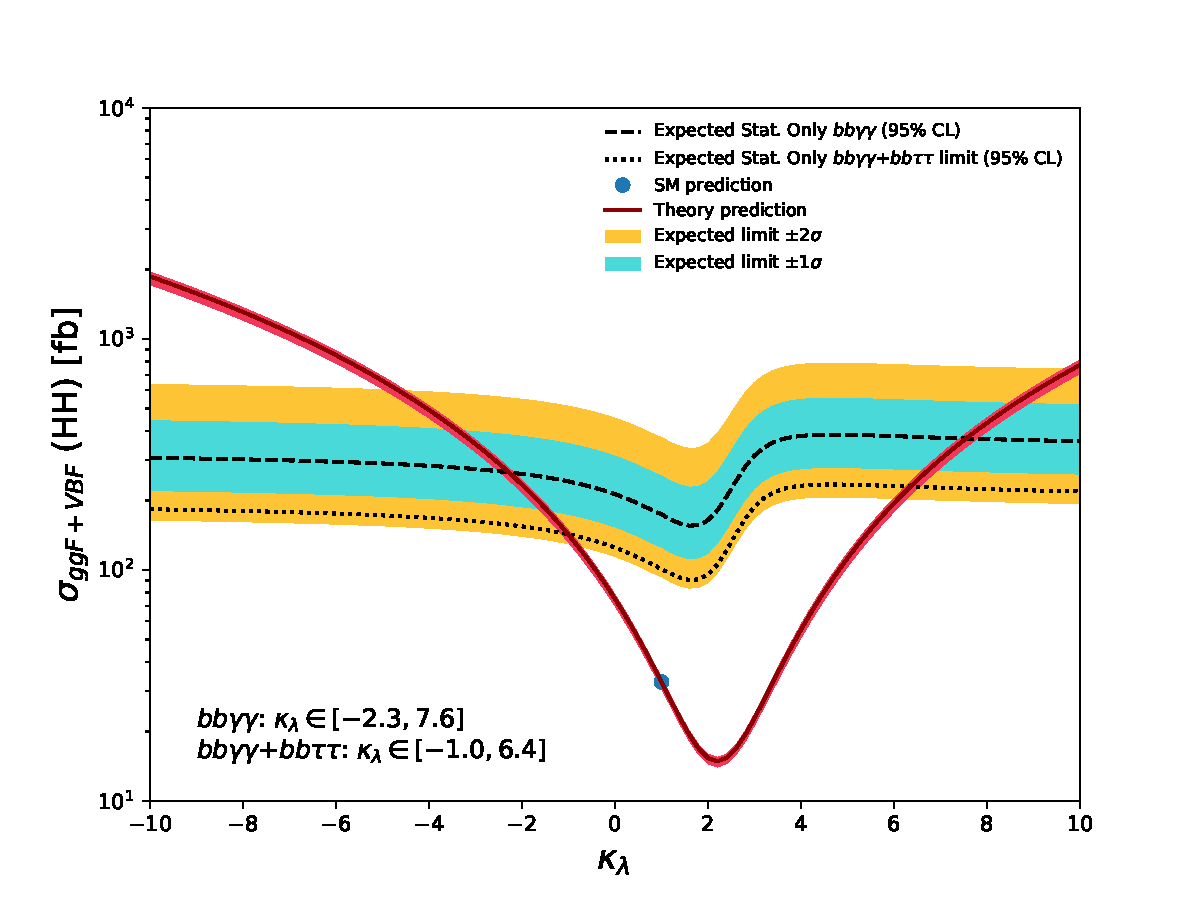
\includegraphics[width=0.6\textwidth]{Ch5/Img/kappa_lambda_bbyy_bbtautau_stat.pdf}
%    \begin{tcolorbox}[colback=black!5!white, colframe=white!75!black]
%    \caption{The stat. only expected 95\% CL upper limits on the HH cross-section obtained for different values of \kl. The \bbtt+\bbyy expected limits are obtained by scaling the \bbyy luminosity with a factor of 2.4. The $\pm$1 and $\pm$2 bands are shown for the \bbyy limits.}
%    \label{fig:HHyybb:HH:tt:Comb}
%    \end{tcolorbox}
%\end{figure}

\subsection{Combination}

A combination of the three channels for 36 \ifb was published to set a better constraint on \kl and the HH production cross-section \cite{HH_Comb_36}. In this combination, the \bbbb and \bbtt channels were combined with the 36 \ifb \bbyy to set the constraint on \kl parameter. Other channels are also considered for the cross-section limit combination such as $\bar{b}bW^+W^-$, $\bar{b}b\gamma\gamma$ and $W^+W^-W^+W^-$ but with limited gain. Figure \ref{fig:HHyybb:comb:xsec} shows the upper limits for individual final states and their combination. The combined observed (expected) upper limit on the SM HH production is 6.9 (10) times the SM prediction. The sensitivity of the SM HH is driven by the \bbbb, \bbtt and \bbyy modes which explains the motivation to consider only these three channels for the \kl constraint. 
\begin{figure}[htbp]
    \centering
    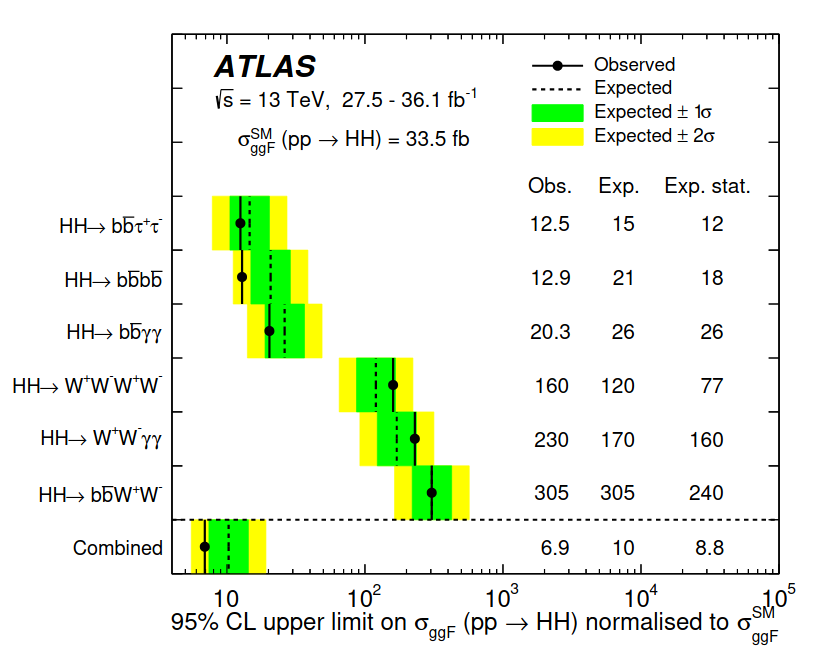
\includegraphics[width=0.6\textwidth]{Ch1/Img/XSec_Comb_36.png}
    \caption{Upper limits at 95\% CL on the ggF SM HH production normalized to its SM expectation from the \bbtt, \bbbb, \bbyy, $\bar{b}bW^+W^-$, $\bar{b}b\gamma\gamma$ and $W^+W^-W^+W^-$ decay channels, and their combination.}
    \label{fig:HHyybb:comb:xsec}
\end{figure}

The upper limit as a function of \kl is shown in Figure \ref{fig:HHyybb:comb:kl}. In the \bbtt final state the observed limit is more stringent than the expected limits over the whole range of \kl, due to a deficit in data relative to the background predictions at high values of the BDT score. The \bbyy limit shows a weaker dependence on \kl than the \bbbb and \bbtt limits because its acceptance is less dependent on \kl. The combination results are summarized in Table \ref{tab:HHyybb:Comb:XSEC}.

\begin{figure}[htbp]
    \centering
    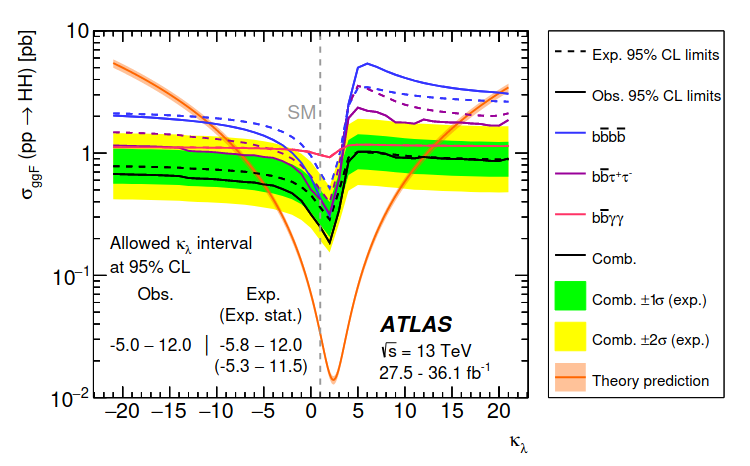
\includegraphics[width=0.65\textwidth]{Ch1/Img/Klambda_Comb_36.png}
    \caption{Upper limits at 95\% CL on the cross-section of the ggF SM HH production as a function of \kl.}
    \label{fig:HHyybb:comb:kl}
\end{figure}

\begin{table}[htbp]
    \centering
    \begin{tabular}{lcc}
    \hline\hline
         & Observed & Expected \\
    \hline
        $\sigma_{gg\rightarrow HH}$/$\sigma^{SM}_{gg\rightarrow HH}$ & 6.9 & 10 \\
        Allowed \kl interval & [-5.0, 12.0] & [-5.8, 12.0] \\
    \hline\hline
    \end{tabular}
    \caption{The 95\% CL observed and expected limits on the Higgs boson pair cross-section normalized to the SM production cross-section and the allowed \kl interval.}
    \label{tab:HHyybb:Comb:XSEC}
\end{table}
%The combination of the full Run-2 analysis would improve the upper limit on the Higgs pair production cross-section. 

\section{Conclusion}

The full Run-2 \HHyybb analysis sets the best constraint to date on the Higgs boson self-coupling. The previous results are improved by a factor of 2.4 on top of the improvement due to the integrated luminosity increase. The improvement is mainly coming from the analysis strategy by dividing events in sub-categories of $m_{HH}$, implementing machine learning to increase separation between signal and background and improving the $b$-jet energy resolution. The developed $b$-jet energy calibration leads to an improvement of 10\% on the analysis significance. The presented full Run-2 \HHyybb analysis sets a slightly better constraint than the full Run-2 CMS analysis and the combined 36 \ifb results. No HH event is observed in the full Run-2 data, neither by ATLAS nor CMS. The observed limit at 95\% CL on HH cross-section is set to 4.2 times the SM prediction and an allowed \kl interval to [-1.5, 6.7]. The results are better than the 36 \ifb combining all decay channels. New data taking period is foreseen at the LHC Run-3 (and beyond) in which an additional integrated luminosity of 300 \ifb is expected with the same pile up conditions. The HL-LHC program with 20 times more data than Run-2 as described in Section \ref{chap2:Upgrad}. The next chapter is dedicated to discuss the possible improvements and prospective for the HH search at Run-3 and HL-LHC. 